%& -shell-escape 

\documentclass[a4paper,11pt]{book}

\usepackage[utf8]{inputenc}
\usepackage{graphicx}
\usepackage{amsmath}
\usepackage{amssymb}
\usepackage{amsthm}
\usepackage{tikz}
\usepackage{tkz-fct}
\usepackage{framed}
\usepackage{systeme}
\usepackage{hieroglf}
\usepackage{bm}
\usepackage{mathtools}
\usepackage{enumerate}
\usepackage{subcaption}
\usepackage[framemethod=TikZ]{mdframed}
\usepackage{tabstackengine}
\usepackage[titletoc]{appendix}
\usepackage{stmaryrd}
\usepackage{xr-hyper}
\usepackage{hyperref}

% This helps with column vectors.
\setstackgap{L}{1.3\baselineskip}
% This helps with matrices
\setstacktabbedgap{1.5ex}


\newtheorem{theorem}{Theorem}
\newtheorem{corollary}[theorem]{Corollary}
\newtheorem{lemma}[theorem]{Lemma}
\newtheorem{proposition}[theorem]{Proposition}
\theoremstyle{definition}
\newtheorem{definition}[theorem]{Definition}
\newtheorem{exercise}{Exercise}
\newtheorem{example_environment}{Example}[chapter]
\newtheorem{remark}[theorem]{Remark}
\newtheorem*{solution}{Solution}

\newcommand{\be}{\begin{equation}}
\newcommand{\ee}{\end{equation}}
\newcommand{\ba}{\begin{aligned}}
\newcommand{\ea}{\end{aligned}}
\newcommand{\bt}{\begin{aligned} \begin{tikzpicture}}
\newcommand{\et}{\end{tikzpicture} \end{aligned}}
\newcommand{\ve}[1]{\mathbf{#1}}
\newcommand{\mat}[1]{\mathsf{#1}}
\newcommand{\col}[1]{\bm{\mat{#1}}}
\newcommand{\basis}[1]{{\mathcal #1}}
\newcommand{\cvector}[1]{\bracketVectorstack{#1}}
\newcommand{\cmatrix}[1]{\bracketMatrixstack{#1}}
\newcommand{\dotp}{\boldsymbol{\cdot}}


\newcommand{\furtherexercises}{\section*{Further exercises for \thesection}}
\newenvironment{example}
	{
		\begin{oframed} 
		\begin{example_environment}
	}
	{
		\end{example_environment}
		\end{oframed}
	}

% Custom made symbols for a list not just a set
\newcommand{\bmark}{\raisebox{.53ex}{\rule{.2em}{.1ex}}}
\newcommand{\bopen}{{\protect\ooalign{\{\cr\hfil\bmark\hfil\cr}}}
\newcommand{\bclose}{{\protect\ooalign{\}\cr\hfil\bmark\hfil\cr}}}



\DeclareMathOperator{\Fun}{Fun}
\DeclareMathOperator{\Cont}{Cont}
\DeclareMathOperator{\Diff}{Diff}
\DeclareMathOperator{\Poly}{Poly}
\DeclareMathOperator{\Trig}{Trig}
\DeclareMathOperator{\Mat}{Mat}
\DeclareMathOperator{\Col}{Col}
\DeclareMathOperator{\id}{id}
\DeclareMathOperator{\vc}{vec}
\DeclareMathOperator{\Dim}{Dim}
\DeclareMathOperator{\Ker}{Ker}
\DeclareMathOperator{\Nullity}{Nullity}
\DeclareMathOperator{\Rank}{Rank}

\let\Im\relax
\DeclareMathOperator{\Im}{Im} % overriding the standard way Im is displayed.


% The "ramanujan says" environment

\definecolor{mycolor}{RGB}{117,192,175}

\tikzstyle{mybox} = [draw=mycolor, very thick,
    rectangle, rounded corners, inner sep=10pt]
\tikzstyle{fancytitle} =[rounded corners]


\newenvironment{ramanujansays}{
 \mdfsetup{%
    frametitle={%
        \tikz[baseline=(current bounding box.east),outer sep=0pt]
        \node[anchor=east,rectangle,fill=none]
        {\strut 
\includegraphics[width=25pt]{smallraj.png}};}
        }
 	\mdfsetup{%
    	innertopmargin=-5pt, innerbottommargin=10pt,
		linecolor=mycolor,%
    	linewidth=2pt,topline=true,%
    	frametitleaboveskip=-20pt, nobreak=true
	}
 
\begin{mdframed}[]\relax%
}
{\end{mdframed}}


\begin{document}

\frontmatter


\author{{\Large Bruce Bartlett}  \\ {\large Afrikaans translation by Murray Heymann}}
\title{Linear Algebra W214}
\date{\today}



\maketitle

\setcounter{tocdepth}{1}
\tableofcontents



\chapter{Note for the student} \label{Ch0NoteForStudent}

You are about to meet linear algebra for the second time. In the first year, we focused on systems of linear equations, matrices, and their determinants. That was good and well, but the time has come for you to return to these topics from a more abstract, mathematical viewpoint. 

You should not be scared by {\em abstraction}. It simply means getting rid of extraneous detail and limiting oneself exclusively to the most important features of a problem. This allows you to understand the problem better. There are less things to worry about! Moreover, if you encounter another problem, which is superficially different but shares the same important features as the original problem, then you could understand it in the same way. This is the power of abstraction.

When we study abstract mathematics, we use the language of {\em definitions}, {\em theorems} and {\em proofs}. Learning to think along these lines (developing abstract mathematical thinking) can be a daunting task at first. But keep trying. One day it will `click' into place and you will realize it is all much more simple than you had first imagined. 

You cannot read mathematics the way you read a novel. You need to have a {\em pencil and notepad} with you, and you need to actively {\em engage} with the material. For instance, if you encounter a definition, start by writing down the definition on your notepad. Just the act of writing it out can be therapeutic! 

If you encounter a worked example, try to write out the example yourself. Perhaps the example is trying to show that $A$ equals $B$. Start by asking yourself: Do I understand what `$A$' actually means? Do I understand what `$B$' actually means? Only then are you ready to consider the question of whether $A$ is equal to $B$ !

Good luck in this new phase of your mathematical training. Enjoy the ride!










\mainmatter

\chapter{Abstract vector spaces} \label{Ch1AbstractVectorSpaces}

\section{Introduction} \label{Ch1Sec1Intro}

\subsection{Three different sets}

We start by playing a game. Recall that in mathematics, a {\em set} $X$ is just a collection of distinct objects. We call these objects the {\em elements} of $X$.

I am going to show you three different sets, and you need to tell me the properties that they all have in common.

The first set, $A$, is defined to be the set of all ordered pairs $(x,y)$ where $x$ and $y$ are real numbers.


\begin{ramanujansays}
Let us pause for a second and translate this definition from English into mathematical symbols. The translation is:
 \be
A := \{ (a_1,\, a_2) : a_1,a_2 \in \mathbb{R}  \} .
 \ee 
The $:=$ stands for `is defined to be'. The $\{$ and $\}$ symbols stand for `the set of all'. The lone colon $:$ stands for `where' or `such that'. The comma in between $a$ and $b$ stands for `and'. The $\in$ stands for `an element of'. And $\mathbb{R}$ stands for the set of all real numbers. 

Well done --- you are learning the language of mathematics!
\end{ramanujansays}

An element of $A$ is an arbitrary pair of real numbers $\ve{a} = (a_1, \, a_2)$. For instance, $(1, \, 2) \in A$ and $(3.891,  \, e^\pi)$ are elements of $A$. Note also that I am using a boldface $\ve{a}$ to refer to an element of $A$. This is so that we can distinguish $\ve{a}$ from its {\em components} $a_1$ and $a_2$, which are just ordinary numbers (not elements of $A$). 

We can visualize an element $\ve{a}$ of $A$ as a point in the Cartesian plane whose $x$-coordinate is $a_1$ and whose $y$-coordinate is $a_2$:
tikzalign
\begin{align*}
{\color{red} \ve{a}} \quad \xrightarrow{\mbox{visualize as}} \quad
\begin{tikzpicture}[baseline={([yshift=-.5ex]current bounding box.center)},vertex/.style={anchor=base,
	circle,fill=black!25,minimum size=18pt,inner sep=2pt}]
\draw[<->] (-2, 0) -- (2,0) node[right] {$x$};
\draw[<->] (0, -2) -- (0, 2) node[above] {$y$};
\node [circle, fill=black, inner sep=0pt, minimum size=5pt, color=red] (P) at (1.3, 1) {};
%	\draw[->, thick] (0,0) -- (1.3, 1);
\draw[dotted] (1.3, 0) node[below] {$a_1$} -- (1.3, 1);
\draw[dotted] (0, 1) node[left] {$a_2$} -- (1.3, 1);
\node[color=red] at (1.6,1) {$\ve{a}$};
\end{tikzpicture}
\end{align*}



The second set, $B$, is defined to be the set of all ordered real triples $(b_1, \, b_2, \, b_3)$ satisfying $b_1 - b_2 + b_3 = 0$. Translated into mathematical symbols,
\be
 B := \{ (b_1, \, b_2, \, b_3) : b_1, b_2, b_3 \in \mathbb{R} \mbox{ and } b_1 - b_2 + b_3 = 0\} .
\ee
For instance, $(2,3, 1) \in B$ but $(1,1,1) \notin B$. We can visualize an element $\ve{b}$ of $B$ as a point in the plane in 3-dimensional space carved out by the equation $x-y+z = 0$:
tikzalign
\begin{align*}
{\color{red} \ve{b}} \quad \xrightarrow{\mbox{visualize as}} \quad
\begin{tikzpicture}[baseline={([yshift=-.5ex]current bounding box.center)},vertex/.style={anchor=base,
	circle,fill=black!25,minimum size=18pt,inner sep=2pt}]
\draw[->] (0, 0) -- (2,0) node[right] {$y$};
\draw[->] (0, 0) -- (0, 2) node[above] {$z$};
\draw[->] (0,0) -- (-0.7, -0.8) node[below left] {$x$};
\node [circle, fill=red, inner sep=0pt, minimum size=5pt] (P) at (0.3, 0.9) {};
\node[color=red] at (0.5, 0.9) {$\ve{b}$};
\draw[thick] (-0.1, -1) -- (-1, 0.4);
\draw[thick] (-1, 0.4) -- (0.3, 1.5);
\draw[thick] (0.3, 1.5) -- (1.5, 0.4);
\draw[thick] (1.5, 0.4) -- (-0.1, -1);
\end{tikzpicture}
\end{align*}
The third set, $C$, is the set of all polynomials of degree 4. Translated into mathematical symbols,
\be
 C := \{ \mbox{polynomials of degree $\leq 4$}\}.
\ee
Recall that the {\em degree} of a polynomial is the highest power of $x$ which occurs.  For instance, $\ve{c} = x^4 - 3 x^3 + 2x^2$ is a polynomial of degree 4, and so is $\ve{p} = 2x^3 + \pi x$. So $\ve{c}$ and $\ve{p}$ are elements of $C$. But $\ve{r} = 8x^5 - 7$ and $\ve{s} = \sin(x)$ are not elements of $C$. We can visualize an element $\ve{c} \in C$ (i.e. a polynomial of degree 4) via its {\em graph}. For instance, the polynomial $\ve{c} = x^4 - 3x^3 + 2x^2 \in C$ can be visualized as:
tikzalign
\begin{align*}
{\color{red} \ve{c}} \quad \xrightarrow{\mbox{visualize as}} \quad
\begin{tikzpicture}[baseline={([yshift=-.5ex]current bounding box.center)},vertex/.style={anchor=base,
	circle,fill=black!25,minimum size=18pt,inner sep=2pt},domain=-0.5:2.2]
\draw[<->] (-0.7, 0) -- (2.5,0) node[right] {$x$};
\draw[<->] (0, -0.8) -- (0, 1) node[above] {$y$};    
\draw[color=red, thick] plot[id=p]  (\x, {(\x-2)*\x*\x*(\x-1)}) 
node[right] {$\ve{c}$};
\end{tikzpicture}
\end{align*}


There you have it. I have defined three different sets: $A$, $B$ and $C$, and I have explained how to visualize the elements of each of these sets. On the face of it, the sets are quite different. Elements of $A$ are arbitrary points in $\mathbb{R}^2$. Elements of $B$ are points in $\mathbb{R}^3$ satisfying a certain equation. Elements of $C$ are polynomials.

What features do these sets have in common? 

\subsection{Features the sets have in common}
I want to focus on two features that the sets $A$, $B$ and $C$ have in common. 

\subsubsection{Addition}

Firstly, in each of these sets, there is a natural {\em addition operation}. We can add two elements of the set to get a third element. 

In set $A$, we can add two elements $\ve{a} = (a_1, \, a_2)$ and $\ve{a}' = (a_1', \, a_2')$ together by adding their components together, to form a new element $\ve{a} + \ve{a}' \in A$:
\be \label{add_in_A}
 \underbrace{(a_1, \, a_2)}_{\ve{a}} + \underbrace{(a'_1, \,a'_2)}_{\ve{a}'} := \underbrace{(a_1 + a_1', \, a_2 + a_2')}_{\ve{a} + \ve{a}'}
\ee
For instance, $(1, \,3) + (2, \,-1.6) = (3, \,1.4)$. We can visualize this addition operation as follows:
tikzalign
\begin{align*}
\begin{tikzpicture}[baseline={([yshift=-.5ex]current bounding box.center)},vertex/.style={anchor=base,
	circle,fill=black!25,minimum size=18pt,inner sep=2pt}, scale=0.8]
\draw[<->] (-2, 0) -- (2,0) node[right] {$x$};
\draw[<->] (0, -2) -- (0, 2) node[above] {$y$};
\node [circle, fill=black, inner sep=0pt, minimum size=5pt, color=red] (P) at (1.3, 1) {};
%	\draw[->, thick] (0,0) -- (1.3, 1);
\draw[dotted] (1.3, 0) node[below] {$a_1$} -- (1.3, 1);
\draw[dotted] (0, 1) node[left] {$a_2$} -- (1.3, 1);
\node[color=red] at (1.6,1) {$\ve{a}$};
\end{tikzpicture}
\quad + \quad
\begin{tikzpicture}[baseline={([yshift=-.5ex]current bounding box.center)},vertex/.style={anchor=base,
	circle,fill=black!25,minimum size=18pt,inner sep=2pt}, scale=0.8]
\draw[<->] (-2, 0) -- (2,0) node[right] {$x$};
\draw[<->] (0, -2) -- (0, 2) node[above] {$y$};
\node [circle, fill=black, inner sep=0pt, minimum size=5pt, color=red] (P) at (0.5, 0.3) {};
%	\draw[->, thick] (0,0) -- (1.3, 1);
\draw[dotted] (0.5, 0) node[below] {$a'_1$} -- (0.5, 0.3);
\draw[dotted] (0, 0.3) node[left] {$a'_2$} -- (0.5, 0.3);
\node[color=red] at (0.9,0.4) {$\ve{a}'$};
\end{tikzpicture}
\quad = \quad
\begin{tikzpicture}[baseline={([yshift=-.5ex]current bounding box.center)},vertex/.style={anchor=base,
	circle,fill=black!25,minimum size=18pt,inner sep=2pt}, scale=0.8]
\draw[<->] (-2, 0) -- (2,0) node[right] {$x$};
\draw[<->] (0, -2) -- (0, 2) node[above] {$y$};
\node [circle, fill=black, inner sep=0pt, minimum size=5pt, color=red] (P) at (1.8, 1.3) {};
%	\draw[->, thick] (0,0) -- (1.3, 1);
\draw[dotted] (1.8, 0) node[below] {$a_1+ a'_1$} -- (1.8, 1.3);
\draw[dotted] (0, 1.3) node[left] {$a_2 + a'_2$} -- (1.8, 1.3);
\node[color=red] at (1.8,1.7) {$\ve{a} + \ve{a}'$};
\end{tikzpicture}
\end{align*}



We can do a similar thing in set $B$. Suppose we have two elements of $B$, $\ve{b} = (b_1, \,b_2, \,b_3)$ and $\ve{b}' = (b_1', \, b_2', \, b_3')$. Note that, since $\ve{b}\in B$, its components satisfy $b_1 - b_2 + b_3 = 0$. Similarly the components of $b'$ satisfy and $b_1 - b_2 + b_3 = 0$. We can add $\ve{b}$ and $\ve{b}'$ together to get a new element $\ve{b} + \ve{b}'$ of $B$, by adding their components together as before:
\be \label{new_add_in_B}
 \underbrace{(b_1, \, b_2, \, b_3)}_{\ve{b}} + \underbrace{(b'_1, \,b'_2, \, b'_3)}_{\ve{b}'} := \underbrace{(b_1 + b_1', \, b_2 + b_2', \, b_3 + b'_3)}_{\ve{b} + \ve{b}'}
\ee
We should be careful here. How do we know that the expression on the right hand side is really an element of $B$? We need to check that it satisfies the equation `the first component minus the second component plus the third component equals zero'. Let us check that formally:
\begin{align*}
 (\ve{b} + \ve{b}')_1 - (\ve{b}+\ve{b}')_2 + (\ve{b}+\ve{b}')_3 &= (b_1 + b'_1) - (b_2 + b'_2) + (b_3 + b'_3) \\
 &= (b_1 - b_2 + b_3) + (b'_1 - b'_2 + b'_3) \\
 &= 0 + 0 \\
 &= 0.
\end{align*}
We can visualize this addition operation in $B$ in the same way as we did for $A$.

There is also an addition operation in set $C$. We can add two polynomials together algebraically by adding their corresponding coefficients:
\begin{multline}
  [c_4 x^4 + c_3 x^3 + c_2 x^2 + c_1 x^1 + c_0] + [d_4 x^4 + d_3 x^3 + d_2 x^2 + d_1 x^1 + d_0] \\
  := (c_4 + d_4) x^4 + (c_3 + d_3) x^3 + (c_2 + d_2) x^2 + (c_1 + d_1) x^1 + (c_0 + d_0) \label{add_in_C}
\end{multline}
For instance,
\[
[2x^4  + x^2 - 3x + 2] + [2x^3 - 7x^2 + x] 
= 2x^4 + 2x^3 - 6x^2 -2x + 2.
\]
There is another way to think about the addition of polynomials. Each polynomial $\ve{c}$ can be thought of as a {\em function}, in the sense that we can substitute an arbitrary value of $x$ into the polynomial $\ve{c}$, and it will output a number $\ve{c}(x)$. For instance, if $\ve{c}(x) = 3x^2 - 1$, then $\ve{c}(2) = 11$. If we think of polynomials as functions in this way, then the addition $\ve{c} + \ve{d}$ of two polynomials can be thought of as the new function which, when you substitute some number $x$ into it, outputs $\ve{c}(x) + \ve{d}(x)$. Written mathematically,
\be \label{add_in_C2}
  (\ve{c} + \ve{d})(x) := \ve{c}(x) + \ve{d}(x)
\ee
Thinking in this way, we can visualize the graph of $\ve{c} + \ve{d}$ as the graph of $\ve{c}$ added to the graph of $\ve{d}$:
tikzalign
\begin{multline*}
\begin{tikzpicture}[baseline={([yshift=-.5ex]current bounding box.center)},vertex/.style={anchor=base,
	circle,fill=black!25,minimum size=18pt,inner sep=2pt},domain=-0.5:2.2]
 	\draw[<->] (-0.7, 0) -- (2.5,0) node[right] {$x$};
 	\draw[<->] (0, -0.8) -- (0, 1) node[above] {$y$};    
    \draw[color=red, thick] plot[id=p] (\x, {(\x-2)*\x*\x*(\x-1)})
        node[right] {$\ve{c}$};
    \draw[dotted]  (1.7, 0)  node[above] {$x$} -- (1.7, -0.6069);
    \draw[dotted]  (0, -0.6069)  node[left] {$\ve{c}(x)$} -- (1.7, -0.6069);
\end{tikzpicture}
\quad + \quad
\begin{tikzpicture}[baseline={([yshift=-.5ex]current bounding box.center)},vertex/.style={anchor=base,
	circle,fill=black!25,minimum size=18pt,inner sep=2pt},domain=-0.5:2.2]
 	\draw[<->] (-0.7, 0) -- (2.5,0) node[right] {$x$};
 	\draw[<->] (0, -0.8) -- (0, 1) node[above] {$y$};    
    \draw[color=red, thick] plot[id=p] (\x ,{-0.2*\x*\x})
        node[right] {$\ve{d}$};
   \draw[dotted]  (1.7, 0)  node[above] {$x$} -- (1.7, -0.578);
    \draw[dotted]  (0, -0.578)  node[left] {$\ve{d}(x)$} -- (1.7, -0.578);
\end{tikzpicture} \\ = \quad
\begin{tikzpicture}[baseline={([yshift=-.5ex]current bounding box.center)},vertex/.style={anchor=base,
	circle,fill=black!25,minimum size=18pt,inner sep=2pt},domain=-0.5:2.2]
 	\draw[<->] (-0.7, 0) -- (2.5,0) node[right] {$x$};
 	\draw[<->] (0, -1.8) -- (0, 1) node[above] {$y$};    
    \draw[color=red, thick] plot[id=p] (\x,{(\x-2)*\x*\x*(\x-1) - 0.2*\x* \x})
        node[above right] {$\ve{c}+\ve{d}$};
   \draw[dotted]  (1.7, 0)  node[above] {$x$} -- (1.7, -1.1849);
    \draw[dotted]  (0, -1.1849)  node[left] {$\ve{c}(x) + \ve{d}(x)$} -- (1.7, -1.1849);       
\end{tikzpicture}
\end{multline*}

\subsubsection{Zero element}
In all three sets $A$, $B$ and $C$, there is a specific element (the {\em zero element}) $\ve{0}$ which, when you add it to another element, leaves that element unchanged. 

In $A$, the zero element $\ve{0}$ is defined by
\be \label{zero_in_A}
 \ve{0} := (0,0) \in A.
\ee
When you add this point to another point $(a_1, \, a_2) \in A$, nothing happens! 
\[ 
 (0, \,0) + (a_1, \, a_2) = (a_1, \, a_2).
\]
Do not confuse the zero element $\ve{0} \in A$ with the real number zero, $0 \in \mathbb{R}$. This is another reason why I am using boldface! (You should use underline to distinguish them.)

In $B$, the zero element $\ve{0}$ is the point $(0,0,0) \in B$. When you add this point to another point $(u_1, u_2, u_3) \in B$, nothing happens!
\[
 (0, \, 0, \, 0) + (u_1, \, u_2, \, u_3) = (u_1, \, u_2, \, u_3).
\]
In $C$, the zero element $\ve{0}$ is the {\em zero polynomial}. If we think algebraically, this is the degree polynomial whose coefficients are all zero:
\be \label{zero_in_C}
  \ve{0} = 0 x^4 + 0 x^3 + 0 x^2 + 0 x + 0
\ee
If we think of the polynomial as a function, then the zero polynomial $\ve{0}$ is the function which returns zero for all values of $x$, that is $\ve{0} (x) = 0$ for all $x$. Whichever way we think of it, when we add the zero polynomial to another polynomial, nothing happens!
\begin{multline*}
 [0 x^4 + 0 x^3 + 0 x^2 + 0 x + 0 ] + [c_4 x^4 + c_3 x^3 + c_2 x^2 + c_1 x + c_0] \\
 = [c_4 x^4 + c_3 x^3 + c_2 x^2 + c_1 x + c_0]
\end{multline*}

\subsubsection{Multiplication by scalars}
The last feature all the sets $A$, $B$ and $C$ have in common is that in each set, you can {\em multiply} elements of the set by real numbers. 

For instance, if $\ve{a} = (a_1, a_2)$ is an element of $A$, then we can multiply it by some arbitrary real number, say $9$, to get a new element $9\cdot a$ of $A$. We do this multiplication component-wise:
\be \label{sm_in_A}
  9 \cdot (a_1, \,a_2) := (9 a_1, \, 9a_2).
\ee
In general, if $k \in \mathbb{R}$ is an arbitrary real number, then we can multiply elements $\ve{a} \in A$ by $k$ to get a new element $k \cdot \ve{a} \in A$ by multiplying each component of $\ve{a}$ by $k$:
\[
  \underbrace{k \cdot (a_1, \, a_2)}_{\mbox{\tiny Multiplying a vector by a scalar}} := (\underbrace{k a_1}_{\mbox{\tiny Multiplying two numbers together}}, \, \underbrace{k a_2})
\]
Just be careful to distinguish scalar multiplication $k \cdot \ve{a}$ (written with a $\cdot$) from ordinary multiplication of real numbers $k a_1$ (written with no symbol, just using juxtaposition). Later on, because we are lazy, we will stop writing the $\cdot$ explicitly --- you have been warned!


Visually, this multiplcation operation {\em scales} $\ve{a}$ by a factor of $k$. That is why we call it {\em scalar multiplication}. 


There is a similar scalar multiplication in $B$:
\be \label{sm_in_B}
k (u_1, \, u_2, \, u_3) := (k u_1, \, k u_2, \, k u_3)
\ee

There is also a scalar multiplication operation in $C$. We simply multiply each coefficient of a polynomial $\ve{c} \in C$ by $k$:
\be \label{sm_in_C}
 k \cdot [c_4 x^4 + c_3 x^3 + c_2 x^2 + c_1 x + c_0] = k c_0 x^4 + k c_3 x^3 + k c_2 x^2 + k c_1 x + k c_0
\ee
If we think of the polynomial $\ve{c}$ as a function, then this corresponds to {\em scaling} the graph of the function vertically by a factor of $k$. 

\subsection{Features that the sets do {\em not} have}
Let us mention a few features that the sets do {\em not} have, or at  least do not have in common.

\begin{itemize}
 \item Set $A = \mathbb{R}^2$ has a {\em multiplication operation}. Because we can think of $\mathbb{R}^2$ as the complex plane $\mathbb{C}$, and we know how to multiply complex numbers. There is no clear choice of a multiplication operation on $B$. The same for $C$: if you try to multiply two degree $4$ polynomials in $C$ together, you will get out a polynomial of degree $8$, which does not live in $C$!
 \item There is a {\em `take the derivative'} operation on $C$,
 \[
  \ve{c} \mapsto \frac{d}{dx} \ve{c}
 \] 
 which we will meet again later. Note that taking the derivative decreases the degree of a polynomial by 1, so the result remains in $C$, and so this is a well defined map from $C$ to $C$. There is no analogue of this operation in $A$ and $B$.
 
\begin{ramanujansays}
Note that there is no {\em integration} map from $C$ to $C$, because integrating a polynomial {\em increases} the degree by $1$, so the result might be a polynomial of degree $5$, which does not live in $C$!
\end{ramanujansays} 
  \end{itemize}

\subsection{Rules}

We have found that each of our three sets $A$, $B$ and $C$ have an {\em addition operation} $+$, a {\em zero vector} $\ve{0}$, and a {\em scalar multiplication} operation $\cdot$. Do these operations satisfy any rules, common to all three sets?

For instance, we can think of the addition operation in $A$ as a function which assigns to each pair of elements $\ve{a}$ and $\ve{a}'$ in $A$ a new element $\ve{a} + \ve{a}'$ in $A$. Does this operation satisfy any rules?

Let us see. Let $\ve{a} = (a_1, \,a_2)$ and $\ve{a}' = (a'_1, \, a'_2)$ be elements of $A$. We can add them in two different orders,
\[
 \ve{a} + \ve{a}' = (a_1 + a'_1, \, a_2 + a'_2)
\]
and
\[
 \ve{a}' + \ve{a} = (a'_1 + a_1, \, a'_2 + a_2) .
\]
Are these the same? In other words, does the rule 
\be \label{comm_in_A}
\ve{a} + \ve{a}' = \ve{a}' + \ve{a}
\ee 
hold? The answer is {\em yes}, but why? To check whether two elements of $A$ are equal, we have to check whether each of their components are equal. The first component of $\ve{a} + \ve{a}'$ is $a_1 + a'_1$. The first component of $\ve{a}' + \ve{a}$ is $a'_1 + a_1$. Is $a_1 + a'_1 = a'_1 + a_1$? Yes --- because these are just ordinary real numbers (not elements of $A$ anymore), and we know that for ordinary real numbers, you can add them together in either order and get the same result. So the first component of $\ve{a} + \ve{a}'$ is equal to the first component of $a'+ a$. Similarly, we can check that the second component of $\ve{a} + \ve{a}'$ is equal to the second component of $\ve{a}' + \ve{a}$. So all the components of $\ve{a} + \ve{a}'$ are equal to all the components of $\ve{a}' + \ve{a}$. So, finally, we conclude that $\ve{a} + \ve{a}' = \ve{a}' + \ve{a}$.

Does this rule \eqref{comm_in_A} also hold for the addition operations in $B$ and $C$?  Yes. For instance, let us check that it holds in $C$. Suppose that $\ve{c}$ and $\ve{d}$ are polynomials in $C$.  Does the rule
\be
 \ve{c} + \ve{d} = \ve{d} + \ve{c} \label{must_check}
\ee
hold? 

The left and right hand sides of \eqref{must_check} are elements of $C$. And elements of $C$ are polynomials. To check if two polynomials are equal, we need to check if they are equal {\em as functions}, in other words, if you get identical results output from both functions no matter what input value of $x$ you substitute in. 

At an arbitrary input value $x$, the left hand side computes as $(\ve{c} + \ve{d})(x) = \ve{c}(x) + \ve{d}(x)$. On the other hand, the right hand side computes as $(\ve{d} + \ve{c})(x) = \ve{d}(x) + \ve{c}(x)$. Now, remember that $\ve{c}(x)$ and $\ve{d}(x)$ are just ordinary numbers (not polynomials). So $\ve{c}(x) + \ve{d}(x) = \ve{d}(x) + \ve{c}(x)$, because this is true for ordinary numbers. So for each input value $x$, $(\ve{c} + \ve{d}) (x) = (\ve{d} + \ve{c})(x)$. Therefore the polynomials $\ve{c} + \ve{d}$ and $\ve{d} + \ve{c}$ are equal, because they output the same values for all numbers $x$.

There are other rules that also hold in all three sets. For instance, in all three sets, the rule
\be
 (\ve{x} + \ve{y}) + \ve{z} = \ve{x} + (\ve{y} + \ve{z})
\ee
holds for any three elements $\ve{x}$, $\ve{y}$ and $\ve{z}$. Can you find the other common rules?

\section{Definition of an abstract vector space} \label{Ch1Sec2DefVectorSpace}
Mathematics is about identifying patterns. We have found three different sets, $A$, $B$ and $C$, which look very different on the surface but have much in common. In each set, there is an addition operation, a zero vector, and a scalar multiplication operation. Moreover, in each set, these operations satisfy the same rules. Let us now record this pattern by giving it a name and writing down the rules explicitly. 

\begin{definition}\label{real_vec_space} A {\em vector space} is a set $V$ equipped with the following data: \label{defnvec}
\begin{itemize}
 \item[D1.] An {\em addition operation}. (That is, for every pair of elements $\ve{u}, \ve{v} \in V$, a new element  $\ve{u} + \ve{v} \in V$ is defined.)
 \item[D2.] A {\em zero vector}. (That is, a special vector $\ve{0} \in V$ is marked out.)
 \item[D3.] A {\em scalar multiplication operation}. (That is, for each real number $k$ and each element $\ve{v} \in V$, a new element $k \cdot \ve{v} \in V$ is defined).
\end{itemize}

This data should satisfy the following rules for all $\ve{u}, \ve{v}, \ve{w}$ in $V$ and for all real numbers $k$ and $l$:
 \begin{enumerate}
 	\item[R1.] $\ve{v} + \ve{w} = \ve{w} + \ve{v}$  
	\item[R2.] $(\ve{u} + \ve{v}) + \ve{w} = \ve{u} + (\ve{v} + \ve{w})$
	\item[R3.] a) $\ve{0} + \ve{v} = \ve{v}$ \\ 
	b) $\ve{v} + \ve{0} = \ve{v}$
	\item[R4.] $k \cdot (\ve{v} + \ve{w}) = k \cdot \ve{v} + k \cdot \ve{w}$
	\item[R5.] $(k + l) \cdot \ve{v} = k \cdot \ve{v} + l \cdot {\ve{v}}$
	\item[R6.] $k \cdot (l \cdot \ve{v}) = (kl) \cdot \ve{v}$
	\item[R7.] $1 \cdot \ve{v} = \ve{v}$
	\item[R8.] $0 \cdot \ve{v} = \ve{0}$	
 \end{enumerate}
\end{definition}
We will call the elements of a vector space {\em vectors}, and we will write them in boldface eg. $\ve{v} \in V$. We do this to distinguish vectors from real numbers, which we will call {\em scalars}, and which don't have a boldface. It is difficult to use boldface in handwriting, so you should write them with an arrow on top, like so: $\vec{v}$.

Also, in this chapter we will write scalar multiplication with a $\cdot$, for instance $k \cdot \ve{v}$, but in later chapters we will simply write it as $k \ve{v}$ for brevity, so be careful!

To prove that a certain set can be given the structure of a vector space, one therefore needs to do the following:

\begin{ramanujansays}
\begin{enumerate}
 \item Define a set $V$.
 \item Define the data of an addition operation (D1), a zero vector (D2), and a scalar multiplication operation (D3) on $V$. 
  \item Check that this data satisfies the rules (R1) - (R8).
\end{enumerate}
\end{ramanujansays}

\section{First example of a vector space} \label{Ch1Sec3ExampleVectorSpace}

We were led to the definition (Definition \ref{defnvec}) of an abstract vector space by considering the properties of sets $A$, $B$ and $C$ in Section \ref{intro1}. Let us check, for instance, that $B$ indeed satisfies Definition \ref{defnvec}. The others will be left as exercises.
tikc
\begin{example} The set $B$ is a vector space.
\subsubsection{1. Define a set $B$}
We define
\be \label{def_of_b}
 B := \{ (u_1, \, u_2, \, u_3) : u_1, u_2, u_3 \in \mathbb{R} \mbox{ and } u_1 - u_2 + u_3 = 0\} .
\ee

\subsubsection{2. Define addition, the zero vector, and scalar multiplication}
D1. We define addition as follows. Suppose $\ve{u} = (u_1, \, u_2, \, u_3)$ and $\ve{v} = (v_1, , v_2, \, v_3)$ are elements of $B$. Note that in particular this means $u_1 - u_2 + u_3 = 0$ and $v_1 - v_2 + v_3 = 0$. We define $\ve{u} + \ve{v}$ by:
\be \label{def_add_in_B}
 \ve{u} + \ve{v} := (u_1 + v_1, \, u_2 + v_2, \, u_3 + v_3).
\ee
We need to check that this makes sense. We are supposed to have that $\ve{u} + \ve{v}$ is also an element of $B$. We can't just write down any definition! To check if $\ve{u} + \ve{v}$ is an element of $B$, we need to check if it satisfies equation \eqref{def_of_b}. Let us check:
\begin{align*}
 &(u_1 + v_1) - (u_2 + v_2) + (u_3 + v_3) \\
 &= (u_1 - u_2 + u_3) + (v_1 - v_2 + v_3) && \mbox{(this algebra step is true for ordinary numbers)} \\
 &= 0 + 0 && \mbox{(since $\ve{u}$ and $\ve{v}$ are in $B$)} \\
 &= 0.
\end{align*}
Therefore, $\ve{u} + \ve{v}$ is indeed an element of $B$, so we have written down a well-defined addition operation on $B$, which takes two arbitrary elements of $B$ and outputs another element of $B$. \\

\noindent D2. We define the zero vector $\ve{0} \in B$ as
\be \label{zero_vec_in_B}
 \ve{0} := (0, 0, 0).
\ee
We need to check that this makes sense. Does $(0,0,0)$ really belong to $B$,in other words, does it satisfy equation \eqref{def_of_b}? Yes, since $0 - 0 + 0 = 0$. So we have a well-defined zero vector. \\

\noindent D3. We define scalar multiplication on $B$ as follows. Let $k$ be a real number and $\ve{u} = (u_1, \, u_2, \, u_3)$ be an element of $B$. We define
\be \label{s_mu_in_B}
  k \cdot \ve{u} := (ku_1, \, ku_2, \, ku_3).
\ee
We need to check that this makes sense. When I multiply a multiply a vector $\ve{u}$ in $B$ by a scalar $k$, the result $k \cdot \ve{u}$ is supposed to be an element of $B$. Does $(ku_1, \, ku_2, \, ku_3)$ really belong to $B$? Let us check that it satisfies the defining equation \eqref{def_of_b}:
\begin{align*}
	& ku_1 - ku_2 + ku_3  \\
	&= k (u_1 - u_2 + u_3) && \mbox{(this algebra step is true for ordinary numbers)} \\
	&= k 0 && \mbox{(since $\ve{u}$ is in $B$)} \\
	&= 0.
\end{align*}
Therefore, $k \cdot \ve{u}$ is indeed an element of $B$, so we have written down a well-defined scalar multiplication operation on $B$. 

\subsubsection{3. Check that the data satisfies the rules}
We must check that our data D1, D2 and D3 satisfies the rules R1 -- R8. So, suppose $\ve{u} = (u_1, \, u_2, \,u_3)$, $\ve{v} = (v_1, \, v_2, \, v_3)$ and $\ve{w} = (w_1, \, w_2, \, w_3)$ are in $B$, and suppose that $k$ and $l$ are real numbers. \\

\noindent R1. We check: 
\begin{align*}
& \ve{v} + \ve{w}\tag{R1.} \\ 
& = (v_1 + w_1, \, v_2 + w_2, \, v_3 + w_3) && \mbox{(by defn of addition in $B$)} \\
& = (w_1 + v_1, \, w_2 + v_2, \, w_3 + v_3) && \mbox{\begin{minipage}{5cm}(because $x + y = y + x$ is true for real numbers)\end{minipage}} \\
&= \ve{w} + \ve{v}. && \mbox{(by defn of addition in $B$)}
\end{align*}

\noindent R2. We check:
\begin{align*}
 & (\ve{u} + \ve{v}) + \ve{w} \\
 &= ( u_1 + v_1, \, u_2 + v_2, \, u_3 + v_3) + \ve{w} && \mbox{(by defn of addition in $B$)} \\
 &= ( (u_1 + v_1) + w_1, \, (u_2 + v_2) + w_2, \, (u_3 + v_3) + w_3) && \mbox{(by defn of addition in $B$)} \\
 &= ( u_1 + (v_1 + w_1), \, u_2 + (v_2 + w_2), \, u_3 + (v_3 + w_3)) && \mbox{\begin{minipage}{5cm}(since $(x + y) + z = x + (y + z)$ is true for real numbers)\end{minipage}}  \\
 &= \ve{u} + (v_1 + w_1, \, v_2 + w_2, \, v_3 + w_3) && \mbox{(by defn of addition in $B$)} \\
 &= \ve{u} + (\ve{v} + \ve{w}) && \mbox{(by defn of addition in $B$)}.
\end{align*}

\noindent R3. We check:
\begin{align*}
 &\ve{0} + \ve{v}  \\
 &= ( 0, \, 0, \, 0) + (v_1, \, v_2, \, v_3) && \mbox{(by defn of the zero vector in $B$}\\
 &= (0 + v_1, \, 0 + v_2, \, 0 + v_3) && \mbox{(by defn of addition in $B$)} \\
 &= (v_1, \, v_2, \, v_3) && \mbox{(because $x + 0 = x$ is true for real numbers)} \\
 &= \ve{v}.
\end{align*}
By the same reasoning, we can check that $\ve{v} + \ve{0} = \ve{v}$. \\

\noindent R4. We check:
\begin{align*}
  & k \cdot ( \ve{v + w} ) \\
  &= k \cdot (v_1 + w_1, \, v_2 + w_2, \, v_3 + w_3) && \mbox{(by defn of addition in $B$} \\
  &= (k (v_1 + w_1, \, k (v_2 + w_2), \, k (v_3 + w_3) ) && \mbox{(by defn of scalar multipliation in $B$)} \\
  &= (kv_1 + kw_1, \, kv_2 + kw_2, \, kv_3 + kw_3) && \mbox{(since $k(x+y) = kx + ky$ for real numbers $x,y$)} \\
  &= (kv_1, \, kv_2, \, kv_3) + (kw_1, \, kw_2,\, kw_3) && \mbox{(by defn of addition in $B$)} \\
  &= k \cdot \ve{v} + k \cdot \ve{w} && \mbox{(by defn of scalar multiplication in $B$)} 
\end{align*} 

\noindent R5. We check:
\begin{align*}
  & (k + l) \cdot \ve{v} \\
  &= ( (k+l) v_1, \, (k+l) v_2,  \, (k+l) v_3) && \mbox{(by defn of scalar multiplication in $B$)} \\
  &= (kv_1 + lv_1, \, kv_2 + lv_2, \, kv_3 + lv_3) && \mbox{(since $(k+l)x = kx + lx$ for real numbers)} \\
  &= (kv_1, \, kv_2, \, kv_3) + (lv_1, \, lv_2, \, lv_3) && \mbox{(by defn of addition in $B$)} \\
  &= k \cdot \ve{v} + l \cdot \ve{v} && \mbox{(by defn of scalar multiplication in $B$)}
\end{align*} 

\noindent R6. We check:
\begin{align*}
  & k \cdot (l \cdot \ve{v}) \\
  &= k \cdot (l v_1, \, l v_2, \, lv_3) && \mbox{(by defn of scalar multiplication in $B$)} \\ 
  &= (k (lv_1), \, k (lv_2), \, k (lv_3)) && \mbox{(by defn of scalar multiplication in $B$)} \\
  &= ( (kl) v_1, \, (kl) v_2, \, (kl) v_3) && \mbox{(since $k(lx) = (kl)x$ for real numbers)} \\
  &= (kl) \cdot \ve{v} && \mbox{(by defn of scalar multiplication in $B$)}. 
 \end{align*} 

\noindent R7. We check:
\begin{align*}
 1 \cdot \ve{v} &= (1v_1, \, 1v_2, \, 1v_3) && \mbox{(by defn of scalar multiplication in $B$)} \\
 &= (v_1, \, v_2, \, v_3) && \mbox{(since $1 x = x$ for real numbers $x$)} \\
 &= \ve{v}.
 \end{align*}
 
\noindent R8. We check:
\begin{align*}
 0 \cdot \ve{v} &= (0v_1, \, 0v_2, \, 0v_3) && \mbox{(by defn of scalar multiplication in $B$)} \\
 &= (0, \, 0, \, 0) && \mbox{(since $0 x = 0$ for real numbers} \\
 &= \ve{0} && \mbox{(by defn of the zero vector in $B$)}.
 \end{align*}
\end{example}

\furtherexercises

\begin{exercise} Prove that set $A$ from Section \ref{intro1} together with the addition operation \eqref{add_in_A}, the zero vector \eqref{zero_in_A} and the scalar multiplication operation \eqref{sm_in_A} forms a vector space.
\end{exercise}

\begin{exercise} Prove that set $C$ from Section \ref{intro1} together with the addition operation \eqref{add_in_C}, the zero vector \eqref{zero_in_C} and the scalar multiplication operation \eqref{sm_in_C} forms a vector space.
\end{exercise}




\section{More examples and non-examples} \label{Ch1Sec4MoreExamples}

\begin{example}[A non-example] Define the set $V$ by 
\be
 V := \{ \mathbf{a}, \mathbf{b} \} .
\ee
Define the addition operation by 
\begin{align}
 \ve{a} + \ve{a} := \ve{a} && \ve{a} + \ve{b} := \ve{a} \\
 \ve{b} + \ve{a} := \ve{b} && \ve{b} + \ve{b} := \ve{c} 
\end{align}
For this to be a well-defined addition operation, we need to check that whenever you add two elements of $V$ together, you get out a well-defined element of $V$. But $\ve{b} + \ve{b} = \ve{c}$, so adding $\ve{b} \in V$ to itself outputs something, namely $\ve{c}$, which is not an element of $V$. So $V$ does not form a vector space since it does not even have a well-defined addition operation.
\end{example}

\begin{example}[Another non-example] Define the set $V$ by 
\be
 V := \{ \mathbf{a}, \mathbf{b} \} .
\ee
Define the addition operation by 
\begin{align}
 \ve{a} + \ve{a} := \ve{a} && \ve{a} + \ve{b} := \ve{b} \label{ne_11} \\
 \ve{b} + \ve{a} := \ve{b} && \ve{b} + \ve{b} := \ve{a} \label{ne_12}
\end{align}
This is a well-defined addition operation, since whenever you add two elements of $V$ together, you get out a well-defined element of $V$.

Define the zero vector by 
\be
 \ve{0} := \ve{a}. \label{ne_13}
\ee
This is well-defined, since $\ve{a}$ is indeed an element of $V$.

Define scalar multiplication by a real number $k \in \mathbb{R}$ by
\be
 k \cdot \ve{a} := \ve{a} \quad \mbox{and} \quad k \cdot \ve{b} := \ve{b}. \label{ne_14}
\ee
This is a well-defined scalar multiplication, since it allows us to multiply any element $\ve{v} \in V$ by a scalar $k$ and it outputs a well-defined element $k \cdot \ve{v} \in V$. 
\begin{exercise} Show that these operations satisfy rules R1, R2, R3, R4, R6 and R7, but not R5 and R8.
\end{exercise}
\end{example}


\begin{example}[The zero vector space] Define the set $Z$ by 
\be
Z := \{ \ve{z} \}.
\ee 
Note that it contains just a single element, $\ve{z}$.  Define the addition operation as 
\be
 \ve{z} + \ve{z} := \ve{z}
\ee
Define the zero element as
\be
 \ve{0} := \ve{z}.
\ee
Finally define scalar multiplication by a scalar $k \in \mathbb{R}$ as:
\be
 k \cdot \ve{z} := \ve{z}.
\ee
\begin{exercise} Show that this data satisfies the rules R1 to R8. 
\end{exercise}

\end{example}

\begin{example}[$\mathbb{R}^n$] Define the set $\mathbb{R}^n$ by
\be
 \mathbb{R}^n := \{ (x_1, \, x_2, \, \ldots, \, x_n) : x_i \in \mathbb{R} \mbox{ for all } i = 1 \ldots n\}.
\ee
Define the addition operation as
\be
(x_1, \, x_2, \, \ldots, \, x_n) + (y_1, \, y_2, \, \ldots, \, y_n) := (x_1 + y_1, \, x_2 + y_2, \, \ldots, \, x_n + y_n).
\ee
Define the zero element as
\be
 \ve{0} := (0, \, 0, \, \ldots, \, 0).
\ee
Define scalar multiplication by
\be
 k \cdot (x_1, \, x_2, \, \ldots, \, x_n) := (k x_1, \, k x_2, \, \ldots, \, k x_n).
\ee
\begin{exercise} Show that this data satisfies the rules R1 to R8. 
\end{exercise}
\end{example}

\begin{example}[$\mathbb{R}^\infty$] Define the set $\mathbb{R}^\infty$ by
\be
 \mathbb{R}^\infty := \{ (x_1, \, x_2, \, x_3, \, \ldots, ) : x_i \in \mathbb{R} \mbox{ for all } i = 1, 2, 3, \ldots\}
\ee
So an element $\ve{x} \in \mathbb{R}^\infty$ is an infinite sequence of real numbers. Define the addition operation componentwise: 
\be
(x_1, \, x_2, \, x_3, \, \ldots) + (y_1, \, y_2, \, y_3, \, \ldots) := (x_1 + y_1, \, x_2 + y_2, \, x_3 + y_3, \, \ldots).
\ee
Define the zero element as
\be
 \ve{0} := (0, \, 0, \, 0, \, \ldots ),
\ee
the infinite sequence whose components are all zero. Finally, define scalar multiplication componentwise:
\be
 k \cdot (x_1, \, x_2, \, x_3, \, \ldots) := (kx_1, \, kx_2, \, kx_3, \, \ldots)
\ee
\begin{exercise} Show that this data satisfies the rules R1 to R8.
\end{exercise}

\begin{ramanujansays} Thinking about infinity is an important part of mathematics. Have you watched the movie about me called {\em The man who knew infinity}?
\end{ramanujansays}
\end{example}


\begin{example}[Functions on a set] Let $X$ be any set. Define the set $\Fun(X)$ of {\em real-valued functions on $X$} by
\be
	\Fun(X) := \{ \mathbf{f} : X \rightarrow \mathbb{R} \}.
\ee
Note that the functions can be arbitrary; there is no requirement for them to be continuous, or differentiable. Such a requirement would not make sense, since $X$ could be an arbitrary set. For instance $X$ could be the set $\{a, b, c\}$ ---without any further informaiton, it does not make sense to say that a function $\mathbf{f} : X \rightarrow \mathbb{R}$ is continuous.

Define the addition operation by
\be
 (\mathbf{f} + \mathbf{g}) (x) := \mathbf{f}(x) + \mathbf{g}(x), \quad x \in X
\ee
Make sure you understand what this formula is saying! We start with two functions $\mathbf{f}$ and $\mathbf{g}$, and we are defining their sum $\mathbf{f} + \mathbf{g}$. This is supposed to be another function on $X$. To define a function on $X$, I am supposed to write down what value it outputs for each $x \in X$. And that is what the formula says: the value that the function $\mathbf{f} + \mathbf{g}$ assigns to the element $x \in X$ is defined to be the number $\mathbf{f}(x)$ plus the number $\mathbf{g}(x)$. Remember: $\mathbf{f}$ is a function, while $\mathbf{f}(x)$ is a number!

Define the zero vector $\mathbf{0}$ to be the function which outputs the number $0$ for every input value of $x \in X$:
\be
 \ve{0} (x) := 0 \quad \mbox{for all $x \in X$.}
\ee
Define scalar multiplication by
\be
 (k \cdot \mathbf{f})(x) := k \mathbf{f}(x).
\ee
\begin{exercise} Notation quiz! Say whether the following combination of symbols represents a real number or a function.
	\begin{enumerate}
	\item $\mathbf{f}$
	\item $\mathbf{f}(x)$
	\item $k \cdot \mathbf{f}$
	\item $(k \cdot \mathbf{f})(x)$
	\end{enumerate}
\end{exercise}

\begin{exercise} Let $X = \{a, b, c\}$. 
	\begin{enumerate}
		\item Write down three different functions $\mathbf{f}, \mathbf{g}, \mathbf{h}$ in $\Fun(X)$. 
		\item For the functions you constructed in (i), calculate $\mathbf{f} + \mathbf{g}$ as well as $3 \cdot \mathbf{h}$.
	\end{enumerate}
\end{exercise}

\begin{exercise} Show that the data above satisfies the rules R1 to R8, so that $\Fun(X)$ is a vector space.
\end{exercise}
\end{example}


\begin{example}[Matrices] \label{matrices_example_vec_space} the set $\Mat_{n, m}$ of all $n \times m$ matrices is a vector space. See Appendix \ref{reminder-matrices-chap} for a reminder about matrices.

\begin{exercise} Show that when equipped with the addition operation, zero vector, and scalar multiplication operation as defined in Appendix \ref{reminder-matrices-chap}, the set $\Mat_{n, m}$ of all $n \times m$ matrices is a vector space. 
\end{exercise}
\end{example}

\begin{example} We will write $\Col_n$ for the vector space $\Mat_{n,1}$ of $n$-dimensional {\em column vectors},
\[
 \Col_n = \left\{ \left[ \begin{array}{c} x_1 \\ x_2 \\ \vdots \\ x_n \end{array} \right] : x_1, \ldots, x_n \in \mathbb{R} \right\}
\]
So, $\Col_n$ `is' just $\mathbb{R}^n$, but we make explicit the fact that the components of the vectors are arranged in a column. 
\end{example}



\furtherexercises
\begin{exercise} \label{non_ass_ex} Define an addition operation on the set $X := \{ \ve{0}, \, \ve{a}, \, \ve{b} \}$ by the following table:
\[
 \begin{array}{c|ccc}
 	+ & \ve{0} & \ve{a} & \ve{b} \\ 
 	\hline
 	\ve{0} & \ve{0} & \ve{a} & \ve{b} \\
 	\ve{a} & \ve{a} & \ve{0} & \ve{a} \\
 	\ve{b} & \ve{b} & \ve{a} & \ve{0}
 \end{array}
\]
This table works as follows. To calculate, for example, $\ve{b} + \ve{a}$, find the intersection of the row labelled by $\ve{b}$ with the column labelled by $\ve{a}$. We see that $\ve{b} + \ve{a} := \ve{a}$. 

Prove that this addition operation satisfies R1.
\end{exercise}

\begin{exercise} Prove that the addition operation from Exercise \ref{non_ass_ex} does not satisfy R2.
\end{exercise}

\begin{exercise} Define a strange new addition operation $\hat{+}$ on $\mathbb{R}$ by 
\[
 \ve{x} \hat{+} \ve{y} := \ve{x} - \ve{y}, \qquad \ve{x}, \ve{y} \in \mathbb{R}.
\]
Does $\hat{+}$ satisfy R2? If it does, prove it. If it does not, give a counterexample.
\end{exercise}

\begin{exercise} Let $\mathbb{R}^+$ be the set of positive real numbers. Define an addition operation, a zero vector and a scalar multiplication on $\mathbb{R}^+$ by
\begin{align*}
  \ve{x} + \ve{y} &:= \ve{x} \ve{y} \\
   \ve{0} & := 1 \\
   k \cdot \ve{x} &:= \ve{x}^k
\end{align*}
where $\ve{x}$ and $\ve{y}$ are positive real numbers, and $k$ is a scalar (i.e. an arbitrary real number). 
 \begin{enumerate}
 	\item Check that these operations are well-defined. For instance, is $\ve{x} + \ve{y} \in \mathbb{R}^+$, as it should be?
 	\item Check that they satisfy R1 to R8, so that $\mathbb{R}^+$ is a vector space with these operations.
 \end{enumerate}

\end{exercise}

\section{Some results about abstract vector spaces} \label{Ch1Sec5ResultsVectorSpace}
It is time to use the rules of a vector space to prove some general results.

\begin{ramanujansays} We are about to do our first formal proof in the course!
\end{ramanujansays}

\begin{lemma} Suppose $V$ is a vector spaces with zero vector $\ve{0}$. If $\ve{0}'$ is another vector satisfying R3(a),
\be \label{uniqueness_zero}
 \ve{0}' + \ve{v} = \ve{v} \mbox{\, for all $\ve{v} \in V$} 
\ee
then $\ve{0} = \ve{0}'$. 
\end{lemma}
\begin{proof}
\begin{align*}
 \ve{0} &= \ve{0}' + \ve{0} && \mbox{(using \eqref{uniqueness_zero}) for $\ve{v} = \ve{0}$)} \\
 &= \ve{0}' && \mbox{(using R3(b) for $\ve{v} = \ve{0}'$)}
\end{align*}
\end{proof}

\begin{definition} If $V$ is a vector space, we define the {\em additive inverse} of a vector $\ve{v} \in V$ as
\[
 - \ve{v} := (-1) \cdot \ve{v}
\]
\end{definition}

\begin{lemma} If $V$ is a vector space, then for all $\ve{v} \in V$, \label{add_inv}
\be
-\ve{v} + \ve{v} = \ve{0} \mbox{ and } \ve{v} + (-\ve{v}) = \ve{0}.
\ee
\end{lemma}
\begin{proof}
\begin{align*}
	-\ve{v} + \ve{v} &= (-1) \cdot \ve{v} + \ve{v} && \mbox{(using defn of $- \ve{v}$)} \\
	&= (-1) \cdot \ve{v} + 1 \cdot \ve{v} && \mbox{(R7)} \\
	& = (-1 + 1) \cdot \ve{v} && \mbox{(R5)} \\
	&= 0 \cdot \ve{v} \\
	&= \ve{0} && \mbox{(R8)}
\end{align*}
In addition,
\begin{align*}
	\ve{v} + (-\ve{v}) &= -\ve{v} + \ve{v} && \mbox{(R1)} \\
	& = \ve{0} && \mbox{(by previous proof)} \\
\end{align*}
\end{proof}

\begin{lemma} Suppose that two vectors $\ve{w}$ and $\ve{v}$ in a vector space satisfy $\ve{w} + \ve{v} = \ve{0}$. Then $\ve{w} = -\ve{v}$.
\end{lemma}
\begin{proof}
\begin{align*}
	\ve{w} &= \ve{w} + \ve{0} && \mbox{(R3b)} \\
	&= \ve{w} + (\ve{v} + -\ve{v}) && \mbox{(by Lemma \ref{add_inv})} \\ 
	&= (\ve{w} + \ve{v}) + -\ve{v}) && \mbox{(R2)} \\ 
	&= \ve{0} + -\ve{v} && \mbox{(by assumption)} \\
	&= -\ve{v} && \mbox{(R3a)}.	
\end{align*}
\end{proof}

\begin{example} \label{explicit_solve_x} Let us practice using the rules of a vector space to perform everyday calculations. For instance, suppose that we are trying to solve for the vector $\ve{x}$ appearing in the following equation:
\be
 \ve{v} + 7 \cdot \ve{x} = \ve{w}
\ee
We do this using the rules as follows:
\begin{align*}
	 \ve{v} + 7 \cdot \ve{x} & = \ve{w} \\
	\therefore  -\ve{v} + (\ve{v} + 7 \cdot \ve{x}) & = -\ve{v} + \ve{w} && \mbox{(Added $-\ve{v}$ on left to both sides)} \\
	\therefore  (-\ve{v} + \ve{v}) + 7 \cdot \ve{x} & = -\ve{v} + \ve{w} && \mbox{(used R2 on LHS)} \\
	\therefore  \ve{0} + 7 \cdot \ve{x} & = -\ve{v} + \ve{w} && \mbox{(used Lemma \ref{add_inv} on LHS)} \\
	\therefore  7 \cdot \ve{x} & =  -\ve{v} + \ve{w} && \mbox{(used R3a on LHS)} \\
	\therefore  \frac{1}{7} \cdot (7 \cdot \ve{x}) & = \frac{1}{7} \cdot (-\ve{v} + \ve{w}) && \mbox{(scalar multiplied both sides by $\frac{1}{7}$)} \\
	\therefore  (\frac{1}{7} 7) \cdot 	\ve{x} & = \frac{1}{7} \cdot (-\ve{v} + \ve{w}) && \mbox{(used R6 on LHS)} \\
	\therefore  1 \cdot \ve{x} & =  \frac{1}{7} \cdot (-\ve{v} + \ve{w})  && \mbox{(multiplied $\frac{1}{7}$ with $7$)} \\
	\therefore  \ve{x} & =  \frac{1}{7} \cdot (-\ve{v} + \ve{w}) && \mbox{(R7)} 
\end{align*}
As the course goes on we will leave out all these steps. But it is important for you to be able to reproduce them all, if asked to do so!
\end{example}
We will need one final lemma.
\begin{lemma} \label{dichotomy_lem} Suppose that $\ve{v}$ is a vector in a vector space $V$ and that $k$ is a scalar. Then
\[
 k \cdot \ve{v} = \ve{0} \quad \Leftrightarrow \quad k = 0 \mbox{ or } \ve{v} = \ve{0}.
\]
\end{lemma}
\begin{proof} (Proof of $\Leftarrow$). Suppose $k=0$. Then $k \cdot \ve{v} = 0 \cdot \ve{v} = \ve{0}$ by R8 of a vector space. On the other hand, suppose $\ve{v} = \ve{0}$. Then $k \cdot \ve{v} = k \cdot \ve{0} = \ve{0}$ by Exercise \ref{imp_ex_1}. 

(Proof of $\Rightarrow$). Suppose $k \cdot \ve{v} = \ve{0}$. There are two possibilities: either $k = 0$, or $k \neq 0$. If $k=0$, then we are done. If $k \neq 0$, then $\frac{1}{k}$ exists and we can multiply both sides by it:
\begin{align*}
 	 k \cdot \ve{v} & = \ve{0} \\
 	\therefore  \frac{1}{k} \cdot (k \cdot \ve{v})  & = \frac{1}{k} \cdot \ve{0} && \mbox{(Multiplied both sides by $\frac{1}{k}$)} \\
 	\therefore (\frac{1}{k} k) \cdot \ve{v} &= \ve{0} && \mbox{\begin{minipage}{5cm} (On the LHS, we used R6. \\ On the RHS, we used Exercise \ref{imp_ex_1}.) \end{minipage} } \\
 	\therefore 1 \cdot \ve{v} &= \ve{0} && \mbox{(using $\frac{1}{k} k = 1$)} \\
 	\therefore \ve{v} &= \ve{0} && \mbox{(R7)} 
\end{align*}	
Hence in the case $k \neq 0$ we must have $\ve{v} = \ve{0}$, which is what we wanted to show.
\end{proof}



\furtherexercises
\begin{exercise} Prove that for all vectors $v$ in a vector space, $-(-\ve{v}) = \ve{v}$.
\end{exercise}


\begin{exercise} \label{mult_by_zero_ex} Let $V$ be a vector space with zero vector $\ve{0}$. Prove that for all scalars $k$, $k \cdot \ve{0} = \ve{0}$. \label{imp_ex_1}
\end{exercise}

\begin{exercise} Suppose that two vectors $\ve{x}$ and $\ve{w}$ in a vector space satisfy $2 \ve{x} + 6 \ve{w} = \ve{0}$. Solve for $\ve{x}$, showing explicitly how you use the rules of a vector space, as in Example \ref{explicit_solve_x}.
\end{exercise}

\section{Subspaces} \label{Ch1Sec6Subspaces}
The notion of a subspace will allow us to quickly establish many more examples of vector spaces.
\begin{definition}A subset $U \subseteq V$ of a vector space $V$ is called a {\em subspace of $V$} if:
\begin{itemize} \item For all $\ve{u}, \ve{u}' \in U$, $\ve{u}+\ve{u}' \in U$
\item $\ve{0} \in U$
\item For all scalars $k$ and all vectors $\ve{u} \in U$, $k \cdot \ve{u} \in U$
\end{itemize}
\end{definition}
\begin{lemma} If $U$ is a subspace of a vector space $V$, then $U$ is also a vector space, when we equip it with the same addition operation, zero vector and scalar multiplication as in $V$. \label{subspace_lem}
\end{lemma}
\begin{proof} Since $U$ is a subspace, we know that it actually makes sense to ``equip it with the same addition operation, zero vector and scalar multiplication as in $V$''. (If $U$ was {\em not} a subspace, then we might have for instance $\ve{u}, \ve{u}' \in U$ but $\ve{u}+\ve{u}' \notin U$, so the addition operation would not make sense.)

So we simply need to check the rules R1 to R8. Since these rules hold for all vectors $\ve{u}, \ve{v}, \ve{w}$ in $V$, they certainly hold for all vectors $\ve{u}, \ve{v}, \ve{w}$ in $U$. So R1 to R8 are satisfied.
\end{proof}

\begin{example}[Line in $\mathbb{R}^2$] A line $L$ through the origin in $\mathbb{R}^2$ is a subspace of $\mathbb{R}^2$:
\be \label{pic_of_L1}
\ba
\begin{tikzpicture}
	\draw[<->] (-2, 0) -- (2,0) node[below] {$x$};
	\draw[<->] (0, -2) -- (0, 2) node[right] {$y$};
	\draw[thick, red] (-2, -1) -- (2, 1) node[below] {$L$};
\end{tikzpicture}
\ea
\ee
Indeed, recall that $L$ can be specified by a homogenous linear equation of the form:
\be \label{eqn_of_L}
 L = \{ (x,y) \in \mathbb{R}^2 : ax + by = 0 \}
\ee
for some constants $a$ and $b$. So, if $\ve{v} = (x, \, y)$ and $\ve{v}' = (x', \, y')$ lie on $L$, then their sum $\ve{v} + \ve{v}' = (x + x', \, y + y')$ also lies on $L$, because its components satisfy the defining equation \eqref{eqn_of_L}:
\begin{align*}
 &a(x + x') + b (y + y')\\
 & = (ax + by) + (ax' + by') \\
 &= 0 + 0 && \mbox{(since $ax + by = 0$ and $ax' + by' = 0$)} \\
 &= 0.
\end{align*}
This also makes sense geometrically: if you look at the picture \eqref{pic_of_L1}, then you will see that adding two vectors $\ve{v}, \ve{v}'$ on $L$ by the head-to-tail method will produce another vector on $L$.  
\begin{exercise} Complete the proof that $L$ is a subspace of $\mathbb{R}^2$ by checking that the zero vector is in $L$, and that multiplying a vector in $L$ by a scalar outputs a vector still in $L$.
\end{exercise}
\end{example}

\begin{example}[Lines and planes in $\mathbb{R}^3$] Similarly a line $L$ or a plane $P$ through the origin in $\mathbb{R}^3$ is a subspace of $\mathbb{R}^3$:
\be \label{pic_of_L}
\ba
\begin{tikzpicture}
 	\draw[->] (0, 0) -- (2,0) node[right] {$y$};
	\draw[->] (0, 0) -- (0, 2) node[above] {$z$};
	\draw[->] (0,0) -- (-0.7, -0.8) node[below left] {$x$};
	\draw[thick, red] (-2, 1) node[above] {$L$} -- (2, -1);
\end{tikzpicture}
\ea
\qquad \qquad
\ba
\begin{tikzpicture}
 	\draw[->] (0, 0) -- (2,0) node[right] {$y$};
	\draw[->] (0, 0) -- (0, 2) node[above] {$z$};
	\draw[->] (0,0) -- (-0.7, -0.8) node[below left] {$x$};
	\draw[thick, red] (-0.1, -1) -- (-1, 0.4);
	\draw[thick, red] (-1, 0.4) -- (0.3, 1.5);
	\draw[thick, red] (0.3, 1.5) -- node[above right] {$P$} (1.5, 0.4);
	\draw[thick, red] (1.5, 0.4) -- (-0.1, -1);
\end{tikzpicture}
\ea
\ee

\end{example}

\begin{example}[Zero vector space] If $V$ is a vector space, the the set $
\{\ve{0}\} \subseteq V$ containing just the zero vector $\ve{0}$ is a subspace of $V$.
\begin{exercise} Check this.
\end{exercise}
\end{example}

\begin{example}[Non-example: Line not through origin] Be careful though --- not {\em every} line $L \subset \mathbb{R}^2$ is a subspace of $\mathbb{R}^2$. If $L$ does not go through the origin, then $\ve{0} \notin L$, so $L$ is not a subspace. 

Another reason that $L$ is not a subspace is that it is not closed under addition: when we add two nonzero vectors $\ve{v}$ and $\ve{v}'$ on $L$, we end up with a vector $\ve{v} + \ve{v}'$ which does not lie on $L$:
\be \label{pic_of_bad_L}
\ba
\begin{tikzpicture}[scale=2]
	\draw[<->] (-2, 0) -- (2,0) node[below] {$x$};
	\draw[<->] (0, -2) -- (0, 2) node[right] {$y$};
	\draw[thick, red] (-2, -0.5) -- (2, 1.5) node[below] {$L$};
	\draw[very thick, red, ->] (0,0) -- node[left] {$\ve{v}$} (0.5, 0.75);
	\draw[very thick, red, ->] (0,0) -- node[right] {$\ve{v}'$} (1, 1);
	\draw[very thick, red, ->] (0.5,0.75) -- node[above left] {$\ve{v}'$} (1.5, 1.75) node[above right] {$\ve{v} + \ve{v}'$};
\end{tikzpicture}
\ea
\ee
\end{example}



\begin{example}[Continuous functions as a subspace] The set 
\[
 \Cont(I) := \{ \ve{f}: I \rightarrow \mathbb{R}, \, \ve{f} \mbox{ continuous} \}
 \]
of all continuous functions on an interval $I$ is a subspace of the set $\Fun(I)$ of {\em all} functions on $I$. Let us check that it satisfies the definition. You know from earlier courses that:
\begin{itemize}
\item If $\ve{f}$ and $\ve{g}$ are continuous functions on $I$, then $\ve{f} + \ve{g}$ is also a continuous function. 
\item The zero function $\bf{0}$ defined by $\ve{0}(x) = 0$ for all $x \in I$ is a continuous function.
\item If $\ve{f}$ is a continuous function, and $k$ is a scalar, then $k \cdot \ve{f}$ is also continuous.
\end{itemize}
Hence, by Lemma \ref{subspace_lem}, $\Cont(I)$ is a vector space in its own right.
\end{example}

\begin{example}[Differentiable functions as a subspace] Similarly, the set
\[
 \Diff(I) := \{ \ve{f}: I \rightarrow \mathbb{R}, \, \ve{f} \mbox{ differentiable} \}
 \]
of differentiable functions on an open interval $I$ is a subspace of $\Fun (I)$. 
\begin{exercise} Check this. Also, is $\Diff( I)$ a subspace of $\Cont(I)$?
\end{exercise}
\end{example}

\begin{example}[Vector spaces of polynomials]
 A {\em polynomial} is a function $\ve{p} : \mathbb{R} \rightarrow \mathbb{R}$ of the form
\be
 \ve{p}(x) = a_n x^n + a_{n-1}x^{n-1} + \cdots + a_1 x + a_0. \label{formula_poly}
\ee
for some fixed real coefficients $a_0, \ldots, a_n$. Two polynomials $\ve{p}$ and $\ve{q}$ are {\em equal} if they are equal {\em as functions}, that is if $\ve{p}(x) = \ve{q} (x)$ for all $x \in \mathbb{R}$. The {\em degree} of a polynomial is the highest power of $x$ which occurs in its formula.

For example, $2x^3 - x + 7$ is a polynomial of degree 3, while $x^5 - 2$ is a polynomial of degree 5. 
 We write the set of {\em all} polynomials as $\Poly$ and the set of all polynomials having degree less than or equal to $n$ as $\Poly_n$.

\begin{exercise} Check that $\Poly$ and $\Poly_n$ are subspaces of $\Cont (\mathbb{R})$.
\end{exercise}
\end{example} 

\begin{example}[Trigonometric polynomials] \label{trig_poly_example} A {\em trigonometric polynomial} is a function $\ve{T} : \mathbb{R} \rightarrow \mathbb{R}$ of the form
\begin{multline} \label{formula_for_trig_poly}
 \ve{T} (x) = a_0 + a_1 \cos(x) + b_1 \sin(x) + a_2 \cos(2x) + b_2 \sin(2x) + \cdots \\ + a_n \cos(nx) + b_n \sin(nx) \, .
\end{multline}
The {\em degree} of a trigonometric polynomial is the highest multiple of $x$ which occurs inside one of the sines or cosines in its formula. For instance,
\[
 3 - \cos(x) + 6 \sin(3x)
\] 
is a trigonometric polynomial of degree 3. We write the set of {\em all} trigonometric polynomials as $\Trig$ and the set of all trigonometric polynomials having degree less than or equal to $n$ as $\Trig_n$. 

\begin{exercise} Show that $\Trig$ and $\Trig_n$ are subspaces of $\Cont (\mathbb{R})$.
\end{exercise}

\begin{exercise} Consider the function $\ve{f} (x) = \sin^3(x)$. Show that $\ve{f} \in \Trig_3$ by writing it in the form \eqref{formula_for_trig_poly}. Hint: use the identities \label{trig_ex_early}
\begin{align*}
 \sin(A) \sin(B) &= \frac{1}{2}(\cos(A-B) - \cos(A+B)) \\
 \sin(A) \cos(B) &= \frac{1}{2}(\sin(A-B) + \sin(A+B)) \\
 \cos(A)\cos(B) &= \frac{1}{2}(\cos(A-B) + \cos(A+B))
\end{align*}
which follow easily from the addition formulae 
\begin{align*}
\sin(A \pm B) &= \sin A \cos B \pm \cos A \sin B \\
\cos(A \pm B) &= \cos A \cos B \mp \sin A \sin B.
\end{align*}
\end{exercise}

\end{example}


\begin{example}[Solutions to linear differential equations] Fix constants $a,b$ and $c$. Let $V \subseteq \Diff(\mathbb{R})$ be the set of all solutions to the following differential equation:
\[
 a \frac{d^2f}{dx^2} + b \frac{df}{dx} + cf = 0
\]
\begin{exercise} Show that $V$ is a subspace of $\Diff(\mathbb{R})$.
\end{exercise} 
\end{example}




\furtherexercises

\begin{exercise} Show that the set 
\[
 V := \{ (a, -a, b, -b) : a, b \in \mathbb{R} \}
\]
is a subspace of $\mathbb{R}^4$.
\end{exercise}

\begin{exercise} Show that the set
\[
 V := \{ \mbox{polynomials of the form } \ve{p}(x) = ax^3 + bx^2 - cx + a, \, a,b,c \in \mathbb{R}\}
\]
is a subspace of $\Poly_3$.
\end{exercise}

\begin{exercise} Let $b \in \mathbb{R}$. Prove that 
\[
V := \{ (x_1, \, x_2, \, x_3) \in \mathbb{R}^3 : 2x_1 - 3x_2 + 5x_3 = b \}
\]
is a subspace of $\mathbb{R}^3$ if and only if $b=0$.
\end{exercise} 

\begin{exercise} Consider the set
\[
 V := \{ \mathbf{f} \in \Diff((-1, 1)) : f'(0) = 2 \}
\]
Is $V$ a subspace of $\Diff((-1,1))$? If you think it is, {\em prove} that it is. If you think it is not, {\em prove} that it is not!
\end{exercise}

\begin{exercise} Consider the set
\[
 V := \{ (x_1, \, x_2, \, x_3, \, \ldots) \in \mathbb{R}^\infty : \lim_{n \rightarrow \infty} x_n = 0 \}
\]
Is $V$ a subspace of $\mathbb{R}^\infty$? If you think it is, {\em prove} that it is. If you think it is not, {\em prove} that it is not! 
\end{exercise}

\begin{exercise} Is $\mathbb{R}^+ := \{ \ve{x} \in \mathbb{R} : \ve{x} \geq 0 \}$ a subspace of $\mathbb{R}$? If you think it is, {\em prove} that it is. If you think it is not, {\em prove} that it is not!
\end{exercise}

\begin{exercise} Give an example of a nonempty subset $U$ of $\mathbb{R}^2$ which is closed under addition and under taking additive inverses (i.e. if $\ve{u}$ is in $U$ then $-\ve{u}$ is in $V$), but $U$ is not a subspace of $\mathbb{R}^2$.
\end{exercise}

\begin{exercise} Give an example of a nonempty subset $V$ of $\mathbb{R}^2$ which is closed under scalar multiplication, but $V$ is not a subspace of $\mathbb{R}^2$.
\end{exercise}

\chapter{Finite-dimensional vector spaces} \label{Ch2FinDimVectorSpaces}
In this course we concentrate on {\em finite-dimensional} vector spaces, which we will define in this chapter. 

\begin{ramanujansays}
{\bf Warning}: From now on, I will use shorthand and write scalar multiplication $k \cdot \ve{v}$ simply as $k \ve{v}$!
\end{ramanujansays}

\section{Linear combinations and span} \label{Ch2Sec1LinearCombinationSpan}
We start with some basic definitions.
\begin{definition} A {\em linear combination} of a finite collection $\ve{v}_1, \ldots, \ve{v}_n$ of vectors in a vector space $V$ is a vector of the form
\be
 a_1 \ve{v}_1 + a_2 \ve{v}_2 + \cdots + a_b \ve{v}_n
\ee
where $a_1, a_2, \ldots, a_n$ are scalars. If all the scalars $a_i$ are $0$, we say that it is the {\em trivial} linear combination.
\end{definition}
\begin{example} In $\mathbb{R}^3$, $(6, 2, -14)$ is a linear combination of $(-3, 1, 2)$ and $(-2, 0, 3)$ because
\[
(6, 2, -14) = 2 (-3, 1, 2) -6 (-2, 0, 3).
\]
\end{example}
\begin{example} In $\mathbb{R}^4$, $(2, -1, 3, 0)$ is not a linear combination of $(1, 3, 2, 0), \, (5, 1, 2, 4)$ and $(-1, 0, 2, 1)$. If it {\em was}, then we would have 
\[
 (-2, -1, 3, 0) = a_1 (1, 3, 2, 0) + a_2 (5, 1, 2, 4) + a_3 (-1, 0, 2, 1)
\]
for some scalars $a_1, a_2, a_3$. In other words, we would have
\[
 (-2, -1, 3, 0) = (a_1 + a_2 + a_3, \, 3a_1 + a_2, \, 2a_1 + 2a_2 + 2a_3, \, 4a_2 + a_3)
\]
which is equivalent to the system of equations
\be \label{no_soln1}
\systeme{a_1 + 5a_2 -a_3 = -2, 3a_1 + a_2 = -1, 2a_1 + 2a_2 + 2a_3 = 3, 4a_2 + a_3 = 0}
\ee
\begin{exercise} Check that the system of equations \eqref{no_soln1} has no solution.
\end{exercise}
\end{example}

\begin{example} Define the functions $\ve{f}, \ve{f}_1, \ve{f}_2 \in \Diff$ by
\[
 \ve{f}(x) = \cos^3 x, \quad \ve{f}_1 (x) = \cos (x), \quad \ve{f}_2 (x) = \cos (3x).
 \]
Then $\ve{f}$ is a linear combination of $\ve{f}_1$ and $\ve{f}_2$ because of the identity $\cos(3x) = \frac{1}{4} (3 \cos x  + \cos(3x))$. See Example \ref{trig_poly_example}. In other words,
\[
  \ve{f} = \frac{3}{4} \ve{f}_1 + \frac{1}{4} \ve{f}_2 .
\]
This example shows that $\ve{f}$ is also a trigonometric polynomial, even though its original formula $\ve{f}(x) = cos(3x)$ was not in the form \eqref{formula_for_trig_poly}. 
\end{example}

\begin{definition} We say that a list of vectors $\ve{v}_1, \ve{v}_2, \ldots, \ve{v}_n$ in a vector space $V$ {\em spans} $V$ if every vector $\ve{v} \in V$ is a linear combination of $\ve{v}_1, \ve{v}_2, \ldots, \ve{v}_n$. 
\end{definition}

\begin{example} $\mathbb{R}^2$ is spanned by
\[
 \ve{e}_1 := (1, \, 0), \, \, \ve{e}_2 := (0, 1)
\]
because every vector $\ve{v} = (a_1, \, a_2)$ can be written as the linear combination
\[
 \ve{v} = a_1 \ve{e}_1 + a_2 \ve{e}_2.
\]
\end{example}
\begin{example} $\mathbb{R}^2$ is also spanned by \label{three_vectors_spanning_R2_example}
\[
 \ve{f}_1 := (-1, 2), \, \ve{f}_2 := (1, 1), \, \ve{f}_3 := (2, -1)
\]
See Figure \ref{spanning_set_R2}. Note that every vector $\ve{v}$ can be written as a linear combination of $\ve{f}_1$, $\ve{f}_2$, $\ve{f}_3$ in more than one way (in fact infinitely many!). For instance,
\begin{align}
 (2, 3) &= 3 \ve{f}_1  - \frac{1}{3} \ve{f}_2 + \frac{8}{3} \ve{f}_3 \label{1st_f_eqn} \\
 (2,3) &= 2 \ve{f}_1 + \frac{2}{3} \ve{f}_2 + \frac{5}{3} \ve{f}_3 \label{2nd_f_eqn}
\end{align}

\begin{exercise} Check equations \eqref{1st_f_eqn} and \eqref{2nd_f_eqn}.
\end{exercise}
\end{example}

\begin{figure}[t] 
	\centering
	\begin{tikzpicture}
	\draw[<->] (-2.5, 0) -- (2.5,0) node[below] {$x$};
	\draw[<->] (0, -2.5) -- (0, 2.5) node[right] {$y$};
	\draw[very thick, red, ->] (0,0) -- (-1, 2) node[above left] {$\ve{f}_1$};
	\draw[very thick, red, ->] (0,0) -- (1, 1) node[above right] {$\ve{f}_2$};
	\draw[very thick, red, ->] (0,0) -- (2, -1) node[below right] {$\ve{f}_3$} ;
	\end{tikzpicture}
	\caption{\label{spanning_set_R2} A list of vectors which spans $\mathbb{R}^2$.}
\end{figure}

\begin{example} $\mathbb{R}^n$ is spanned by  \label{Rn_spanning_set}
\be \label{defn_of_e_i}
\ve{e}_1 := (1, 0, \ldots, 0), \,\,\, \ve{e}_2 := (0, 1, \ldots, 0), \,\,\, \ldots, \,\,\, \ve{e}_n := (0, 0, \ldots, 0, 1)
\ee
because every vector $\ve{v} = (a_1, \,a_2, \, \ldots, \, a_n)$ can be written as the linear combination
\be \label{standard_basis_R_n}
 \ve{v} = a_1 \ve{e}_1 + a_2 \ve{e}_2 + \cdots + a_n \ve{e}_n.
\ee
\begin{exercise} Check equation \eqref{standard_basis_R_n}.
\end{exercise}
\end{example}




\furtherexercises
\begin{exercise} Consider the following polynomials in $\Poly_2$:
\[
 \ve{r}_1 (x) := 3x^2 - 2, \, \ve{r}_2 (x) := x^2 + x, \, \ve{r}_3 (x) := x + 1, \, \ve{r}_4 (x) := x-1
\]
\begin{enumerate}
 \item Can the polynomial $\ve{p}$ with $\ve{p}(x) = x^2 + 1$ be written as a linear combination of $\ve{r}_1$, $\ve{r}_2$, $\ve{r}_3$, $\ve{r}_4$?
 \item If so, in {\em how many ways} can this be done?
\end{enumerate}
\end{exercise}

\begin{exercise} Suppose that the vectors $\ve{e}_1$, $\ve{e}_2$, $\ve{e}_3$ and $\ve{e}_4$ span a vector space $V$. Show that the vectors $\ve{f}_1 := \ve{e}_2 - \ve{e}_1$, $\ve{f}_2 := \ve{e}_3 - \ve{e}_2$, $\ve{f}_3 := \ve{e}_4 - \ve{e}_3$, $\ve{f}_4 := \ve{e}_4$ also span $V$. 
\end{exercise}

\begin{exercise} Show that the polynomials \label{chebyshev_example}
\[
\ve{q}_0 (x) := 1, \,\, \ve{q}_1 (x):= x, \,\, \ve{q}_2(x) := 2x^2 - 1, \,\, \ve{q}_3(x) := 4x^3 - 3x
\]
span $\Poly_3$.
\end{exercise}

\section{Linear independence} \label{Ch2Sec2LinearIndependence}

\begin{definition} A list of vectors $\ve{v}_1, \ve{v}_2, \ldots, \ve{v}_n$ in a vector space $V$ is called {\em linearly independent} if the equation
\be \label{lin_independence_eqn}
  k_1 \ve{v}_1 + k_2 \ve{v}_2 + \cdots k_n \ve{v}_n = \ve{0}
\ee
has only the trivial solution $k_1 = k_2 = \cdots = k_n = 0$. Otherwise, the list of vectors $\ve{v}_1, \ve{v}_2, \ldots, \ve{v}_n$ is called {\em linearly dependent}. 
\end{definition}


\begin{remark} Suppose one of the vectors in the collection $\ve{v}_1$, $\ve{v}_2$, $\ldots$, $\ve{v}_n$ is the zero vector $\ve{0}$; for instance suppose $\ve{v}_1 = \ve{0}$. Then the vectors must be linearly dependent, since the equation \eqref{lin_independence_eqn} has the nontrivial solution $k_1 = 1$, $k_2 = k_2 = \cdots = k_n = 0$. So: {\em a list of linearly independent vectors never contains the zero vector!} \label{remark_about_lin_dependence}
\end{remark}

\begin{remark} \label{crit_ind} The criterion for a list of vectors $\ve{v}_1, \ve{v}_2, \ldots, \ve{v}_n$ to be linearly independent, 
\[
  k_1 \ve{v}_1 + k_2 \ve{v}_2 + \cdots k_n \ve{v}_n = \ve{0} \quad \Rightarrow \quad k_1 = k_2 = \cdots = k_n = 0
\]
is clearly equivalent to the criterion that 
\[
 \begin{minipage}{10cm} { All of the $\ve{v}_i$ are nonzero and none of them can be expressed as a nontrivial linear combination of the others.} \end{minipage}
\]
\end{remark}
\begin{exercise} Prove this last remark.

\end{exercise}

\begin{example} The list of vectors $\ve{f}_1 = (-1, \, 2)$, $\ve{f}_2 = (1, \,1)$ from Example \ref{three_vectors_spanning_R2_example} is linearly independent, because the equation
\[
 k_1 (-1, \, 2) + k_2 (1, \, 1) = (0, \, 0)
\]
is equivalent to the system of equations
\be \label{system_from_r2_example}
\systeme{-k_1 + k_2 = 0, 2k_1 + k_2 = 0}
\ee
which has only the trivial solution $k_1 = 0$ and $k_2 = 0$.
\begin{exercise} Check that \eqref{system_from_r2_example} has only the trivial solution.
\end{exercise}
\end{example}

\begin{example} \label{example_about_lin_dep_1} The list of vectors $\ve{f}_1 = (-1, \, 2)$, $\ve{f}_2 = (1, \,1)$, $\ve{f}_3 = (2, \, -1)$ from Example  \ref{three_vectors_spanning_R2_example} is linearly dependent, because the equation
\be \label{eqn_to_check_lin_ind}
 k_1 (-1, \, 2) + k_2 (1, \, 1) + k_3 (2, \, -1) = (0, \, 0)
\ee
is equivalent to the system of equations
\be \label{system_from_r2_example_new}
\systeme{-k_1 + k_2 + 2k_3 = 0, 2k_1 + k_2 - k_3 = 0}
\ee
which has a one-dimensional vector space of solutions parameterized by $t$, 
\be \label{supposed_soln}
 k_1 = t, \, k_2 = -t, \, k_3 = t, \quad t \in \mathbb{R}.
\ee
\begin{exercise} Check that \eqref{system_from_r2_example_new} has the solution set \eqref{supposed_soln}.
\end{exercise}
For instance, for $t=2$, we have
\[
 2 (-1, \, 2) - 2 (1, \, 1) + 2 (2, \, -1) = (0, \, 0)
\]
so that \eqref{eqn_to_check_lin_ind} has nontrivial solutions.
\end{example}



\begin{example} The list of polynomials  \label{new_basis_for_poly_3}
\[
\ve{q}_0(x) := 1, \,\, \ve{q}_1(x) := x, \,\, \ve{q}_2(x) := 2x^2 - 1, \,\, \ve{q}_3(x) := 4x^3 - 3x
\]
from Example \ref{chebyshev_example} is linearly independent in $\Poly_3$. This is because the equation
\[
k_0 \ve{q}_0 + k_1 \ve{q}_1 + k_2 \ve{q}_2 + k_3 \ve{q}_3 = \ve{0}
\]	
becomes the following equation between polynomials:
\[
 4k_3 x^3 + 2k_2 x^2 + (-3k_3 + k_1) x + (-k_2 + k_0) = 0
\]
This is equivalent to the following system of equations,
\[
 \systeme{ 4k_3 = 0, 2k_2 = 0, -3 k_3 + k_1 = 0 , k_0 - k_2 = 0}
\]
which has only the trivial solution $k_0 = k_1 = k_2 = k_3 = 0$.
\end{example}


At the moment, the definition of a list of vectors being `linearly dependent' is that the list is `not linearly independent'! That might get your head in a knot. Here is a more straightforward way to think about linearly depdendent lists of vectors.
\begin{proposition}[Linear Combination of Preceding Vectors] \label{lin_dependence_prop} Let $\ve{v}_1$, $\ve{v}_2$, $\ldots$, $\ve{v}_n$ be a list of vectors in a vector space $V$. The following statements are equivalent:
\begin{enumerate} \item The list of vectors $\ve{v}_1$, $\ve{v}_2$, $\ldots$, $\ve{v}_n$ is linearly dependent.
\item Either $\ve{v}_1 = \ve{0}$, or for some $r \in \{2, 3, \ldots, n\}$, $\ve{v}_r$ is a linear combination of $\ve{v}_1$, $\ve{v}_2$, $\ldots$, $\ve{v}_{r-1}$.
\end{enumerate}
\end{proposition}
\begin{proof} (1) $\Rightarrow$ (2). Suppose that the list $\ve{v}_1$, $\ve{v}_2$, $\ldots$, $\ve{v}_n$ is linearly dependent. This means that there are scalars $k_1$, $k_2$, $\ldots$, $k_n$, not all zero, such that
\be \label{lin_dep_lem_first_eqn}
 k_1 \ve{v}_1 + k_2 \ve{v}_2 + \cdots + k_n \ve{v}_n = \ve{0}.
\ee
Let $r \in \{1, \,2, \ldots, \, n\}$ be the largest index such that $k_r \neq 0$. (We are told that not all the $k_i$ are zero, so this makes sense.) If $r=1$, then \eqref{lin_dep_lem_first_eqn} is simply the equation
\[
 k_1 \ve{v}_1 = \ve{0}, \quad \mbox{where } k_1 \neq 0.
\]
Therefore $\ve{v}_1 = \ve{0}$ by Lemma \ref{dichotomy_lem}, and we are done. On the other hand, suppose $r \neq 1$. Then \eqref{lin_dep_lem_first_eqn} becomes the equation
\[
 k_1 \ve{v}_1 + k_2 \ve{v}_2 + \cdots + k_r \ve{v}_r = \ve{0}, \quad \mbox{where } k_r \neq 0.
\]
By dividing by $k_r$, we can now solve for $\ve{v}_r$ in terms of the preceding vectors $\ve{v}_1$, $\ve{v}_2$, $\ldots$, $\ve{v}_{r-1}$:
\[
 \therefore \ve{v}_r = - \frac{k_1}{k_r} \ve{v}_1 - \frac{k_2}{k_r} \ve{v}_2 - \cdots - \frac{k_{r-1}}{k_r} \ve{v}_{r-1} \, .
\]
(2) $\Rightarrow$ (1). If $\ve{v}_1 = \ve{0}$, then the list of vectors $\ve{v}_1$, $\ve{v}_2$, $\ldots$, $\ve{v}_n$ is certainly linearly dependent by Remark \ref{remark_about_lin_dependence}. On the other hand, suppose that for some $r \in \{2, 3, \ldots, n\}$, $\ve{v}_r$ is a linear combination of the preceding vectors, that is
\[
 \ve{v}_r = a_1 \ve{v}_1 + a_2 \ve{v}_2 + \cdots + a_{r-1} \ve{v}_{r-1}.
\]
Then clearly
\[
 a_1 \ve{v}_1 + a_2 \ve{v}_2 + \cdots + a_{r-1} \ve{v}_{r-1} - \ve{v}_r + 0 \ve{v}_{r+1} + \cdots + 0 \ve{v}_n = \ve{0}
\]
which shows that the list of vectors $\ve{v}_1$, $\ve{v}_2$, $\ldots$, $\ve{v}_n$ is not linearly independent, since not all the coefficients are zero above --- in particular the coefficient of $\ve{v}_r$ is $-1$.
\end{proof}

\begin{ramanujansays}I call this the `Linear Combination of Preceding Vectors Proposition'. You should give all your theorems names, it helps you to remember them and become familiar with them. 
\end{ramanujansays}

\begin{example} \label{app_of_prop_preceding} We saw in Example \ref{example_about_lin_dep_1} that the list of vectors $\ve{f}_1 = (-1, \, 2)$, $\ve{f}_2 = (1, \,1)$, $\ve{f}_3 = (2, \, -1)$ in $\mathbb{R}^3$ is linearly dependent. Therefore, by Proposition \ref{lin_dependence_prop}, we must have either:
\begin{itemize}
 \item $\ve{f}_1 = \ve{0}$ (not the case), or
 \item $\ve{f}_2$ is a scalar multiple of $\ve{f}_1$ (not the case), or
 \item $\ve{f}_3$ is a linear combination of $\ve{f}_1$ and $\ve{f}_2$, which is true:
 \[
  \ve{f}_3 = - \ve{f}_1 + \ve{f}_2
 \]
\end{itemize}
\end{example}

\begin{proposition}[Bumping Off Proposition] Suppose $\basis{L} = \bopen \ve{l}_1, \ve{l}_2, \ldots, \ve{l}_m \bclose$ is a linearly independent list of vectors in a vector space $V$, and that $\basis{S} = \bopen \ve{s}_1, \ve{s}_2, \ldots, \ve{s}_n \bclose$ spans $V$. Then $m \leq n$. \label{bumping_off_lemma}
\end{proposition}
\begin{proof} Start with the original spanning list of vectors
\be
 \basis{S} = \bopen \,\,  \ve{s}_1, \ve{s}_2, \ldots, \ve{s}_n \bclose
\ee
and consider the `bloated' list
\be \label{bloated_list}
 \basis{S}' = \bopen \ve{l}_1, \ve{s}_1, \ve{s}_2, \cdots, \ve{s}_n \bclose
\ee
Since $\ve{l}_1$ is a linear combination of the $\ve{s}_i$, this list is linearly dependent by Remark \ref{crit_ind}. Thus, by Proposition \ref{lin_dependence_prop} (Linear Combination of Preceding Vectors), one of the $\ve{s}$-vectors, say $\ve{s}_r$, can be expressed as a linear combination of the preceding vectors. We can then remove $\ve{s}_r$ from the list (`bump it off'), and the resulting list
\be
 \basis{S}_1 :=  \bopen \ve{l}_1, \ve{s}_1, \ve{s}_2, \cdots, \hat{\ve{s}_r}, \cdots, \ve{s}_n \bclose \qquad \mbox{($\ve{s}_r$ omitted)}
\ee
still spans $V$. We can go on in this way, each time transferring another one of the $\ve{l}$-vectors into the list, and removing another one of the $\ve{s}$-vectors, to arrive at a new spanning list $\basis{S}_2$, $\basis{S}_3$, $\basis{S}_4$, and so on, where list $\basis{S}_k$ has $(n-k)$ $\ve{s}$-vectors. 

Suppose $m > n$. Then the list $\basis{S}_n$ will consist only of $\ve{l}$-vectors,
\[
 \basis{S}_n: \,\, \ve{l}_1, \ve{l}_2, \ldots, \ve{l}_n
\]
and it spans $V$ by construction. But there are still some $\ve{l}$-vectors $\ve{l}_{n+1}, \ldots \ve{l}_{m}$ left over! This means that $\ve{l}_{n+1}$ is a linear combination of the vectors in $\basis{S}_n$, which contradicts the fact that the list $\bopen \ve{l}_1, \ve{l}_2, \ldots, \ve{l}_m \bclose$ was linearly independent. So we cannot have $m > n$ and hence $m \leq n$.
\end{proof}

\furtherexercises

\begin{exercise}  Show that the list of vectors $(2, \, 3, \, 1)$, $(1, \, -1, \, 2)$, $(7, \, 3, \, c)$ is linearly dependent in $\mathbb{R}^3$ if and only if $c=8$.
\end{exercise}

\begin{exercise} \label{2_by_2_matrices_lin_dep}The list of vectors in $\Mat_{2,2}$ given by
\[
  \ve{v}_1 = \cmatrix{1 & 2 \\ 1 & 1}, \, \ve{v}_2 = \cmatrix{0 & 1 \\ -2 & 1}, \, \ve{v}_3 = \cmatrix{1 & 0 \\ 2 & 3}, \, \ve{v}_4 = \cmatrix{0 & 3 \\ 1 & -1}, \, \ve{v}_5 = \cmatrix{1 & 0 \\ 0 & 1}
\]
is linearly independent (you will prove this in Exercise \ref{checking_matrices_lin_dep}, but for the sake of this question you may assume it to be true). Go through the same steps as in Example \ref{app_of_prop_preceding} to find the first vector in the list which is either the zero vector or a linear combination of the preceding vectors.
\end{exercise}



\section{Basis and dimension} \label{Ch2Sec3BasisDimension}


\begin{definition} A list of vectors $\basis{B} = \bopen \ve{e}_1$, $\ve{e}_2$, $\ldots$, $\ve{e}_n\bclose$ in a vector space $V$ is called a {\em basis} for $V$ if it is linearly independent and spans $V$.
\end{definition}

There is a more direct way to think about a basis.

\begin{proposition}[Bases give coordinates] \label{prop_bases_give_coordinates} A list of vectors $\basis{B} = \bopen \ve{e}_1$, $\ve{e}_2$, $\ldots$, $\ve{e}_n \bclose$ in a vector space $V$ is a basis for $V$ if and only if every vector $\ve{v} \in V$ can be written as a linear combination
\be \label{trying_to_formulate_basis}
 \ve{v} = a_1 \ve{e}_1 + a_2 \ve{e}_2 + \cdots + a_n \ve{e}_n
\ee
in precisely {\em one} way. (That is, for each $\ve{v} \in V$ there {\em \bf exist} scalars $a_1$, $a_2$, $\ldots$, $a_n$ satisfying \eqref{trying_to_formulate_basis}, and that moreover these scalars are {\em \bf unique}). 
\end{proposition}

\begin{ramanujansays} It is important to understand the mathematical phrase `There exists a unique $X$ satisfying $Y$'. It means two things. Firstly, that {\em there does exist an} $X$ which satisfies $Y$. And secondly, that there is {\em no more than one} $X$ which satisfies $Y$. 
\end{ramanujansays}
\begin{ramanujansays} We call the scalars $a_1, a_2, \ldots, a_n$ appearing in \eqref{trying_to_formulate_basis} the {\em coordinates} of $\ve{v}$ in the basis $\ve{e}_1, \ve{e}_2, \ldots, \ve{e}_n$.
\end{ramanujansays}

\begin{proof} $\Rightarrow$. Suppose that the list of vectors $\basis{B} = \bopen \ve{e}_1$, $\ve{e}_2$, $\ldots$, $\ve{e}_n \bclose$ is a basis for $V$. Suppose $\ve{v} \in V$. Since the list of vectors $\basis{B}$  spans $V$, we know that we {\em can} write $\ve{v}$ as a linear combination of the vectors in the list in at least one way,
\be \label{one_way_of_expanding}
 \ve{v} = a_1 \ve{e}_1 + a_2 \ve{e}_2 + \cdots + a_n \ve{e}_n.
\ee
We need to show that this is the {\em only} way to express $\ve{v}$ as a linear combination of the vectors $\ve{e}_i$. Indeed, suppose that we also have
\be \label{second_way_of_expanding}
 \ve{v} = b_1 \ve{e}_1 + b_2 \ve{e}_2 + \cdots + b_n \ve{e}_n.
\ee
Subtracting these two equations gives
\[
 \ve{0} = (a_1 - b_1) \ve{e}_1 + (a_2 - b_2) \ve{e}_2 + \cdots + (a_n - b_n) \ve{e}_n.
\]
Since the list of vectors $\ve{e}_1$, $\ve{e}_2$, $\ldots$, $\ve{e}_n$ is linearly independent, we conclude that
\[
 a_1 - b_1 = 0, \,\, a_2 - b_2 = 0, \,\, \cdots, \,\, a_n - b_n = 0.
\]
That is, $a_1 = b_1$, $a_2 = b_2$, and so on up to $a_n = b_n$, and hence the expansion \eqref{one_way_of_expanding} is unique. 

$\Leftarrow$. Conversely, suppose that every vector $\ve{v}$ can be written as a unique linear combination
\[
 \ve{v} = a_1 \ve{e}_1 + a_2 \ve{e}_2 + \cdots + a_n \ve{e}_n.
\]
The fact that each $\ve{v}$ {\em can} be written as a linear combination of the vectors $\ve{e}_1$, $\ve{e}_2$, $\ldots$, $\ve{e}_n$ means that $\basis{B}$ spans $V$. We still need to show that this list $\basis{B}$ is linearly independent. So, suppose that there exist scalars $b_1$, $b_2$, $\ldots$, $b_n$ such that
\be \label{finding_bs_making_zero}
 b_1 \ve{e}_1 + b_2 \ve{e}_2 + \cdots + b_n \ve{e}_n = \ve{0}.
\ee
We need to show that all the $b_i$ must equal zero. We already know {\em one} possible solution of \eqref{finding_bs_making_zero} : simply set each $b_i = 0$. But we are told that each vector (in particular, the vector $\ve{0}$) can be expressed as a linear combination of the $\ve{e}_i$ in exactly one way. Hence this must be the only solution, i.e. we must have $b_1 = b_2 = \cdots = b_n = 0$, and so the list $\basis{B}$ is linearly independent. 
\end{proof}

\begin{theorem}[Invariance of dimension] \label{inv_dim} If $\basis{B} = \bopen \ve{b}_1, \ve{b}_2, \ldots, \ve{b}_m \bclose$ and $\basis{C} = \bopen \ve{c}_1, \ve{c}_2, \ldots, \ve{c}_n\bclose$ are bases of a vector space $V$, then $m=n$. 
\end{theorem}
\begin{proof}  This is a consequence of Proposition \ref{bumping_off_lemma} (the Bumping Off Proposition). Since the $\ve{b}$-vectors are linearly independent and the $\ve{c}$-vectors span $V$, we have $m \leq n$. On the other hand, since the $\ve{c}$-vectors are linearly independent and the $\ve{b}$-vectors span $V$, we have $n \leq m$. Hence $m=n$.
\end{proof}

\begin{definition} A vector space $V$ is {\em finite-dimensional} if it has a basis. In that case, the {\em dimension} of $V$ is the number of elements in a basis for $V$. A vector space is {\em infinte-dimensional} if it is not finite-dimensional.
\end{definition}

\begin{ramanujansays}
Note that the concept of `dimension of a vector space' is only well-defined because of Theorem \ref{inv_dim}.
\end{ramanujansays}

\begin{example}[Standard basis for $\mathbb{R}^n$]
	\label{standard_basis_R_n_ex}The list of vectors 
\[
\ve{e}_1 := (1, 0, \ldots, 0), \,\,\, \ve{e}_2 := (0, 1, \ldots, 0), \,\,\, \ldots, \,\,\, \ve{e}_n := (0, 0, \ldots, 0, 1)
\]
is a basis for $\mathbb{R}^n$. We already saw in Example \ref{Rn_spanning_set} that this list spans $\mathbb{R}^n$. We need to check that it is linearly independent. So, suppose that
\[
 a_1 \ve{e}_1 + a_2 \ve{e}_2 + \cdots + a_n \ve{e}_n = \ve{0}.
\]
Expanding out the left hand side in components using the definition of the standard basis vectors $\ve{e}_i$, this becomes the equation
\[
 (a_1, 0, 0, \ldots, 0) + (0, a_2, 0, \ldots, 0) + \cdots + (0, 0, 0,
	\ldots, a_n) = (0, 0, 0, \ldots, 0).
\]
In other words, we have
\[
 (a_1, a_2, a_3, \ldots, a_n) = (0, 0, 0, \ldots, 0)
\]
which says precisely that $a_1 = a_2 = a_3 = \cdots = a_n = 0$, which is what we needed to prove. Thus the list of vectors $\ve{e}_1, \ve{e}_2, \ldots, \ve{e}_n$ is linearly independent, and is hence a basis for $\mathbb{R}^n$. So $\mathbb{R}^n$ has dimension $n$.
\end{example}



\begin{example} The list of polynomials
\[
 \ve{p}_0 (x) := 1, \, \ve{p}_1 (x) := x, \, \ve{p}_2 (x) := x^2, \, \ldots, \, \ve{p}_n (x) := x^n 
\]
is a basis for $\Poly_n$, so $\Dim \Poly_n = n+1$. Indeed, this list spans $\Poly_n$ by definition, so we just need to check that it is linearly independent. Suppose that
\[
 a_0 \ve{p}_0 + a_1 \ve{p}_1 + a_2 \ve{p_2} + \cdots + a_n \ve{p}_n = \ve{0}.
\]
{\em This is an equation between functions, so it holds for all $x \in \mathbb{R}$!} In other words, for all $x \in \mathbb{R}$, the following equation holds:
\be \label{root_of_poly}
 a_0 + a_1 x + a_2 x^2 + \cdots + a_n x^n = 0 
\ee 
But, we know from algebra that a polynomial equation of the form \eqref{root_of_poly} with nonzero coefficients has {\em at most} $n$ roots $x_1, x_2, \ldots, x_n$. So, in order for \eqref{root_of_poly} to hold for {\em all} real numbers $x$, the coefficients must be zero, i.e. $a_0 = a_1 = a_2 = \cdots = a_n = 0$, which is what we needed to show.
\end{example}


\begin{example} Suppose $X$ is a finite set. Then $\Fun(X)$ is finite-dimensional, with dimension $|X|$, with basis given by the functions $\ve{f}_a$, $a \in X$, defined by:
\be \label{defn_of_basis_of_functions}
 \ve{f}_a (x) :=  \begin{cases} 1 & \mbox{ if } x = a \\ 0 & \mbox{ otherwise} \end{cases}
\ee
We will prove this in a series of exercises.
\begin{ramanujansays}
The formula on the right hand side of \eqref{defn_of_basis_of_functions} occurs so often in mathematics we give it a symbol of its own, $\delta_{ab}$ (the `Kronecker delta'). This symbol stands for the formula: ``If $a=b$, return a 1. If $a \neq b$, return a $0$''. In this language, we can rewrite the definition of the functions $\ve{f}_a$ as
\be
 \ve{f}_a (x) := \delta_{ax}.
\ee 
\end{ramanujansays}

\begin{exercise} Suppose $X = \left\{\mbox{\pmglyph{\HGi}}, \mbox{\pmglyph{\He}}, \mbox{\pmglyph{\HZxi}} \right\}$. 
\begin{enumerate} \item Evaluate the function $\ve{f}_{\mbox{\tiny \pmglyph{\HGi}}}$ at each $x \in X$.
  \item Show that every function $\ve{f} \in \Fun(X)$ can be written as a linear combination of $\ve{f}_{\mbox{\tiny \pmglyph{\HGi}}}$, $\ve{f}_{\mbox{\tiny \pmglyph{\He}}}$ and $\ve{f}_{\mbox{\tiny \pmglyph{\HZxi}}}$.
\end{enumerate}
\end{exercise}

\begin{exercise} Now let $X$ be an arbitrary finite set. Consider the collection of functions 
\[
\ve{f}_a, \, a \in X
\]
Show that this collection (i) spans $\Fun(X)$ and (ii) is linearly independent.
\end{exercise}

\end{example}



\begin{example} $\Trig_n$ is $(2n+1)$-dimensional, with basis 
\begin{multline}
 \ve{T}_0 (x) := 1, \,\,\, \ve{T}_1 (x) := \cos x, \,  \ve{T}_2 (x) := \sin x, \, \ve{T}_3 (x) := \cos 2x, \\ \ve{T}_4 (x) := \sin 2x, \, \ldots, \, \ve{T}_{2n-1} (x) := \cos nx , \, \ve{T}_{2n} (x) := \sin nx.
\end{multline}
You know that these functions span $\Trig_n$, by definition. They are also linearly independent, though we will not prove this. 

\end{example}

\begin{example} \label{dimension_of_matrix_space_example} The dimension of $\Mat_{n,m}$ is $nm$, with basis given by the matrices 
\[
  \mat{E}_{ij} , \quad i=1 \ldots n, \, j = 1 \ldots m
\]
which have a $1$ in the $i$th row and $j$th column and zeroes everywhere else.

\begin{ramanujansays} Usually $\mat{A}$ is a matrix, and $\mat{A}_{ij}$ is the element of the matrix at position $(i,j)$. But now $\mat{E}_{ij}$ is a matrix in its own right! Its element at position $(k,l)$ will be written as $(\mat{E}_{ij})_{kl}$. I hope you don't find this too confusing. In fact, we can write down an elegant formula for the elements of $\mat{E}_{ij}$ using the Kronecker delta symbol:
\begin{equation} \label{kronecker_for_matrix_basis}
 (\mat{E}_{ij})_{kl} = \delta_{ik} \delta_{jl}
\end{equation}

\end{ramanujansays}
movebackintoramanujansays
\begin{exercise} Check that \eqref{kronecker_for_matrix_basis} is indeed the correct formula for the matrix elements of $\mat{E}_{ij}$.
\end{exercise}
\end{example} 


\begin{example} The standard basis of $\Mat_{2,2}$ is
\[
 \mat{E}_{11} = \left[ \begin{array}{cc} 1 & 0 \\ 0 & 0 \end{array} \right], \, \mat{E}_{12} = \left[ \begin{array}{cc} 0 & 1 \\ 0 & 0 \end{array} \right], \mat{E}_{21} = \left[ \begin{array}{cc} 0 & 0 \\ 1 & 0 \end{array} \right], \mat{E}_{22} = \left[ \begin{array}{cc} 0 & 0 \\ 0 & 1 \end{array} \right]. 
\] 
\end{example}

\begin{example} The standard basis of $\Col_n$ is  
\[
 \col{e}_1 := \left[ \begin{array}{c} 1 \\ 0 \\ \vdots \\ 0 \end{array} \right], \, 
\col{e}_2 := \left[ \begin{array}{c} 0 \\ 1 \\ \vdots \\ 0 \end{array} \right], \, 
\ldots, \,
\col{e}_n := \left[ \begin{array}{c} 0 \\ 0 \\ \vdots \\ 1 \end{array} \right] . 
\]
\end{example}
We now consider dimensions of subspaces of vector spaces. 
\begin{proposition} Let $W$ be a subspace of a finite-dimensional vector space $V$. Then $W$ is finite-dimensional, and $\Dim(W) \leq \Dim(V)$.  \label{dim-of-subspace-prop}
\end{proposition}
\begin{proof} Let $n = \Dim(V)$. If $W = \{ \ve{0} \}$, then the statement is clearly true. Suppose $W \neq \{ \ve{0} \}$. Choose a nonzero vector $\ve{e}_1 \in W$ and form the list $\basis{B}_1 = \bopen \ve{e}_1 \bclose$. If it spans $W$, then we are done. If not, there exists $\ve{e}_2 \in W$ which is not a scalar multiple of $\ve{e}_1$. Now consider the list $\basis{B}_2 = \bopen \ve{e}_1, \ve{e}_2 \bclose$. If it spans $W$, we are done. If not, there exists a vector $\ve{e}_3 \in W$ which is not a linear combination of $\ve{e}_1$ and $\ve{e}_2$. Consider the new list $\basis{B}_3 = \bopen \ve{e}_1, \ve{e}_2, \ve{e}_3 \bclose$. And so on.

This process must eventually terminate. That is, there must exist some $k \geq 1$ such that $\basis{B}_k = \bopen \ve{e}_1, \ldots, \ve{e}_k \bclose$ spans $W$, and hence is a basis for $W$. This is because each list $\basis{B}_i$ is linearly independent (by construction, no vector is a linear combination of the preceding vectors). And it is impossible to construct a linearly independent list of vectors in $W$ (and hence in $V$) which has more than $n$ elements, by the Bumping Off Proposition. This also shows that $k \leq n$. 

\end{proof}
It is good to have an example of an infinite-dimensional vector space.

\begin{proposition} $\Poly$ is infinite-dimensional.
\end{proposition}
\begin{proof} Suppose $\Poly$ is finite-dimensional. This means there exists a finite collection of polynomials $\ve{p}_1, \ve{p}_2, \ldots, \ve{p}_n$ which spans $\Poly$. But, let $d$ be the highest degree of all the polynomials in the list $\ve{p}_1, \ve{p}_2, \ldots, \ve{p}_n$. Then $\ve{p} := x^{d+1}$ is a polynomial which is not in the span of $\ve{p}_1, \ve{p}_2, \ldots, \ve{p}_n$, since adding polynomials together and multiplying them by scalars can never increase the degree. We have arrived at a contradiction. So our initial assumption cannot be correct, i.e. $\Poly$ cannot be finite-dimensional. 
\end{proof}

\begin{example} We will not prove this here, but the following vector spaces are also infinite-dimensional:
\begin{itemize}
 \item $\mathbb{R}^\infty$,
 \item $\Fun(X)$ where $X$ is an infinite set,
 \item $\Cont(I)$ for any nonempty interval $I$, and
 \item $\Diff(I)$ for any open interval $I$.
\end{itemize}
\end{example}



\subsection{Sifting} \label{sifting_subsection}
If we consider the proof of Proposition \ref{bumping_off_lemma} (the `Bumping off' Proposition) carefully, we find that it makes use of a {\em sifting algorithm}. This algorithm can actually be applied to {\em any} list of vectors $\ve{v}_1, \ve{v}_2, \ldots, \ve{v}_n$ in a vector space.  Consider each vector $\ve{v}_i$ in the list consecutively. If $\ve{v}_i$ is the zero vector, or if it is a linear combination of the preceding vectors $\ve{v}_1, \ve{v}_2, \ldots, \ve{v}_{n-1}$, remove it from the list. 

\begin{example} Sift the following list of vectors in $\mathbb{R}^3$:
\begin{align*}
\ve{v}_1 &= (1,2,-1), & \ve{v}_2 &= (0, 0, 0), & \ve{v}_3 &= (3, 6, -3) \\
\ve{v}_4 &= (1, 0, 5), & \ve{v}_5 &= (5, 4, 13), &  \ve{v}_6 &= (1, 1, 0).
\end{align*}
We start with $\ve{v}_1$. Since it is not the zero vector, and is not a linear combination of any preceding vectors, it remains. We move on to $\ve{v}_2$, which is zero, so we remove it. We move on to $\ve{v}_3$, which by inspection is equal to $3 \ve{v}_1$, so we remove it. We move on to $\ve{v}_4$. It is not zero, and cannot be expressed as a multiple of $\ve{v}_1$ (check this), so it remains. We move on to $\ve{v}_5$. We check if it can be written as a linear combination
\[
 \ve{v}_5 = a\ve{v}_1 + b \ve{v}_4
\] 
and find the solution $a=2, b=3$ (check this), so we remove it. Finally we move on to $\ve{v}_6$. We check if it can be written as a linear combination
\[
 \ve{v}_6 = a\ve{v}_1 + b \ve{v}_4
\] 
and find no solutions (check this), so it remains. Our final sifted list is
\[
 \ve{v}_1, \ve{v}_4, \ve{v}_6.
\]
\begin{exercise} Do the three `check this' calculations above.
\end{exercise}
\end{example}

Sifting is a very useful way to construct a basis of a vector space!

\begin{lemma} \label{sift_lemma_basis} If a list of vectors $\ve{v}_1, \ve{v}_2, \ldots, \ve{v}_n$ spans a vector space $V$, then sifting the list will result in a basis for $V$.
\end{lemma}
\begin{proof} At each step, the vector that is removed from the list is either the zero vector, or a linear combination of the vectors before it. So if we remove this vector, the resulting list will still span $V$. Thus by the end of the process, the final sifted list of vectors still spans $V$. 

To see that the final sifted list is linearly independent, we can apply Proposition \ref{lin_dependence_prop}. By construction, no vector in the final sifted list is a linear combination of the preceding vectors (if it was, it would have been removed!). Hence the final sifted list is not linearly dependent, so it must be linearly independent!
\end{proof}

\begin{corollary} Any linearly independent list of vectors $\ve{v}_1, \ve{v}_2, \ldots, \ve{v}_k$ in a finite-dimensional vector space $V$ can be extended to a basis of $V$. \label{first_corollary_please}
\end{corollary}
\begin{proof} Since $V$ is finite-dimensional, it has a basis $\ve{e}_1, \ldots, \ve{e}_n$. Now consider the list 
\[
 L : \ve{v}_1, \ve{v}_2, \ldots, \ve{v}_k, \ve{e}_1, \ve{e}_2, \ldots, \ve{e}_n
\]
which clearly spans $V$. By sifting this list, we will arrive at a basis for $V$, by Lemma \ref{sift_lemma_basis}. Some of the $\ve{e}$-vectors may have been removed. But none of the $\ve{v}$-vectors will have been removed, since that would mean some $\ve{v}_i$ is a linear combination of the preceding vectors $\ve{v}_1, \ldots, \ve{v}_{i-1}$, which is impossible, as $\ve{v}_1, \ldots, \ve{v}_k$ is linearly independent list. Hence after sifting the list $L$ we indeed extend our original list $\ve{v}_1, \ldots, \ve{v}_k$ to a basis of $V$.
\end{proof}
\begin{corollary} \label{lin-ind-implies-basis} If $\ve{v}_1, \ve{v}_2, \ldots, \ve{v}_n$ is a linearly independent list of $n$ vectors in an $n$-dimensional vector space $V$, then it is a basis.
\end{corollary}
\begin{proof} By Corollary \ref{first_corollary_please}, we can extend $\ve{v}_1, \ve{v}_2, \ldots, \ve{v}_n$ to a basis for $V$. But $V$ has dimension $n$, so the basis must contain only $n$ vectors by Theorem \ref{inv_dim} (Invariance of Dimension). So we have not added any vectors at all! Hence our original list was already a basis.
\end{proof}

\begin{example} In Example \ref{new_basis_for_poly_3} we showed that the list of polynomials
 \[
\ve{q}_0 (x) := 1, \,\, \ve{q}_1 (x):= x, \,\, \ve{q}_2(x) := 2x^2 - 1, \,\, \ve{q}_3(x) := 4x^3 - 3x
\]
is linearly independent in $\Poly_3$. Since $\Dim \Poly_3 = 4$, we see that it is a basis of $\Poly_3$. 
\begin{ramanujansays} In Exercise \ref{chebyshev_example}, you showed that $\ve{q}_0, \ldots, \ve{q}_3$ is a basis for $\Poly_3$ by `brute force'. This new method is {\em different}!
\end{ramanujansays}
\end{example}

\furtherexercises

\begin{exercise} \label{exercise_for_new_basis}  Sift the list of vectors  
\begin{align*}
\ve{v}_1 &= (0,0,0), & \ve{v}_2 &= (1, 0, -1), & \ve{v}_3 &= (1, 2, 3) \\
\ve{v}_4 &= (3, 4, 5), & \ve{v}_5 &= (4, 8, 12), &  \ve{v}_6 &= (1, 1, 0).
\end{align*}
\end{exercise}

\begin{exercise} Let $V$ be a vector space of dimension $n$. State whether each of the following statements is true or false. If it is true, prove it. If it is false, give a counterexample. \label{true_false_span_lin_ind}
\begin{itemize}
 \item[(a)] Any linearly independent list of vectors in $V$ contains at most $n$ vectors. 
 \item[(b)] Any list of vectors which spans $V$ contains at least $n$ vectors.
\end{itemize}
\end{exercise}

\begin{exercise} Let $\basis{B} = \bopen \ve{v}_1, \ldots, \ve{v}_n \bclose$ be a linearly independent list of vectors in a vector space $V$. Suppose that $\ve{v}$ is a vector in $V$ which cannot be written as a linear combination of the vectors from $\basis{B}$. Show that the list $\basis{B}' = \bopen \ve{v}_1, \ldots, \ve{v}_n, \ve{v} \bclose$ is still linearly independent. (Hint: Use the Linear Combination of Preceding Vectors Proposition.)
\end{exercise}

\begin{exercise} \label{n_lin_ind_is_basis} Complete the proof of the following lemma.

{\bf Lemma.} Suppose $V$ is a vector space of dimension $n$. Then any linearly independent set of $n$ vectors in $V$ is a basis for $V$.

{\bf Proof.}  Let $\basis{B} = \bopen \ve{v}_1, \ldots, \ve{v}_n \bclose$ be a linearly independent set of vectors in $V$. 

Suppose that $\basis{B}$ is {\em not} a basis for $V$. 

Therefore, $\basis{B}$ does not span $V$, since ... (a) 

Therefore, there exists $\ve{v} \in V$ such that ... (b)

Now, add $\ve{v}$ to the list $\basis{B}$ to obtain a new list $\basis{B}' := $ ... (c)

The new list $\basis{B}'$ is linearly independent because ... (d)

This is a contradiction because ... (e)

Hence, $\basis{B}$ must be a basis for $V$.

\end{exercise}

\begin{exercise} \label{checking_matrices_lin_dep} Use Exercise \ref{true_false_span_lin_ind}(a) to show that the list of matrices in $\Mat_{2,2}$ in Exercise \ref{2_by_2_matrices_lin_dep} is linearly dependent.
\end{exercise}

\begin{exercise} In each case, use the results in Exercises \ref{true_false_span_lin_ind} and \ref{n_lin_ind_is_basis} to determine if $\basis{B}$ is a basis for $V$.
\begin{itemize}
 \item[(a)] $V = \Poly_2$, $\basis{B} = \bopen 2 + x^2, \, 1-x, \, 1 + x - 3x^2, \, x-x^2 \bclose$
 \item[(b)] $V = \Mat_{2,2}$, $\basis{B} = \left\{ \cmatrix{1 & 2 \\ -1 & 3}, \, \cmatrix{0 & 1 \\ 3 & -1}, \, \cmatrix{1 & 2 \\ 3 & 4} \right\}$
 \item[(c)] $V = \Trig_2$, $\basis{B} = \left\{ \sin^2 x, \, \cos^2 x, \, 1 - \sin 2x, \, \cos 2x + 3 \sin 2x  \right\}$
\end{itemize}
\end{exercise}



\begin{exercise} Let $\bopen \ve{u}, \ve{v}, \ve{w} \bclose$ be a linearly independent list of vectors in a vector space $V$. State whether each of the following statements is true or false. If it is true, prove it. If it is false, give a counterexample. (Hint: Use the definition of linear independence.)
\begin{itemize}
 \item[(a)] The list $\bopen \ve{u} + \ve{v}, \, \ve{v} + \ve{w}, \, \ve{u} + \ve{w} \bclose$ is linearly independent.
 \item[(b)] The list $\bopen \ve{u} - \ve{v}, \, \ve{v} - \ve{w}, \, \ve{u} - \ve{w} \bclose$ is linearly independent.
\end{itemize}
\end{exercise}


\begin{exercise} \label{dim_poly_at_2_ex} For each of the following, show that $V$ is a subspace of $\Poly_2$, find a basis for $V$, and compute $\Dim V$.
\begin{itemize}
 \item[(a)] $V = \{ p \in \Poly_2 : p(2) = 0 \}$
 \item[(b)] $V = \{ p \in \Poly_2 : xp'(x) = p(x) \}$
\end{itemize}
\end{exercise}




\section{Coordinate vectors} \label{Ch2Sec4CoordinateVectors}

\begin{definition} Let $\basis{B} = \bopen \ve{b}_1, \ve{b}_2, \ldots, \ve{b}_n \bclose$ be a basis for a vector space $V$, and let $\ve{v} \in V$. Write
\[
 \ve{v} = a_1 \ve{b}_1 + a_2 \ve{b}_2 + \cdots + \ve{a}_n \ve{b}_n \, .
\]
Then the column vector
\[
 [\ve{v}]_\basis{B} := \left[ \begin{array}{c} a_1 \\ a_2 \\ \vdots \\ a_n \end{array} \right] \in \Col_n
\]
is called the {\em coordinate vector of $\ve{v}$ with respect to the basis $\basis{B}$}.
\end{definition}

\begin{ramanujansays} I indicate that a collection of things is a {\em list} (where the order matters) and not merely a {\em set} (where the order does not matter) using my own home-made symbols $\{ \}$. A basis $\basis{B} = \bopen \ve{b}_1, \ve{b}_2, \ldots, \ve{b}_n \bclose$ is a list of vectors. The order of the vectors matters because it affects the coordinate vector $[\ve{v}]_\basis{B}$.
\end{ramanujansays}

\begin{example} Find the coordinate vector of $\ve{p} = 2x^2 - 2x + 3$ with respect to the basis $\basis{B} = \bopen 1+x, x^2 + x -1, x^2 + x + 1\bclose$ of $\Poly_3$.
\begin{solution} We write $\ve{p}$ as a linear combination of polynomials from the basis $\basis{B}$:
\[
2x^2 - 2x + 3 = -4(1+x) - \frac{5}{2} (x^2 + x -1) + \frac{9}{2}(x^2 + x +1)
\]
\begin{exercise} Check this!
\end{exercise}
\[ 
 [\ve{p}]_\basis{B} = \cvector{ -4 \\ - \frac{5}{2} \\ \frac{9}{2} }
\]
\end{solution}
\end{example}

\begin{example} \label{coord_vectors_finding_example}Find the coordinate vectors of $\ve{v}$ and $\ve{w}$ in Figure \ref{v_and_w_in_basis_B} with respect to the basis $\basis{B} = \bopen \ve{b}_1, \ve{b}_2 \bclose$.

\begin{solution} By inspection, we see that $\ve{v} = 2 \ve{b}_1 - \ve{b}_2$, so that
\[
 [\ve{v}]_\basis{B} = \cvector{ 2 \\ -1}
\]
Also by inspection, we see that $\ve{w} = -3 \ve{b}_1 + 2 \ve{b}_2$, so that
\[
 [\ve{v}]_\basis{B} = \cvector{ -3 \\ 2}
\]
\end{solution}

\end{example}
\begin{figure}
	
 \begin{tikzpicture}[scale=0.5]
	\draw[red, dotted] (-9, -9) -- (3, -3);
	\draw[red, dotted] (-8, -7) -- (4, -1);
	\draw[red, dotted] (-7, -5) -- (5, 1);
	\draw[red, dotted] (-6, -3) -- (6, 3);
	\draw[red, dotted] (-5, -1) -- (7, 5);
	\draw[red, dotted] (-4, 1) -- (8, 7);
	\draw[red, dotted] (-3, 3) -- (9, 9);

	\draw[red, dotted] (-9, -9) -- (-3, 3);
	\draw[red, dotted] (-7, -8) -- (-1, 4);
	\draw[red, dotted] (-5, -7) -- (1, 5);
	\draw[red, dotted] (-3, -6) -- (3, 6);
	\draw[red, dotted] (-1, -5) -- (5, 7);
	\draw[red, dotted] (1, -4) -- (7, 8);
	\draw[red, dotted] (3, -3) -- (9, 9);

	
	\draw[very thick, red, ->] (0,0) -- node[pos=1.3] {$\ve{b}_1$} (2,1); 
	\draw[very thick, red, ->] (0,0) -- node[pos=1.3] {$\ve{b}_2$} (1,2);
	\draw[thick, ->] (0,0) -- (3,0) node[below right] {$\ve{v}$};
	\draw[thick, ->] (0,0) -- node[pos=1.2] {$\ve{w}$} (-4,1); 
 \end{tikzpicture}
\caption{\label{v_and_w_in_basis_B}
The basis $B$ for $\mathbb{R}^2$.}
\end{figure}


\begin{example} Find the coordinate vector of the function $\ve{f}$ given by 
\[
 \ve{f}(x) = \sin^2 x - \cos^3 x
\]
with respect to the standard basis
\[
\basis{S} = \bopen 1, \cos x, \sin x, \cos 2x, \sin 2x, \cos 3x, \sin 3x\bclose
\]
of $\Trig_3$.
\begin{solution} Using the addition formulae for $\sin$ and $\cos$ as in Exercise \ref{trig_ex_early}, we compute
\[ 
 \sin^2 x - \cos^3 x = \frac{1}{2} - \frac{3}{4} \cos x - \frac{1}{2} \cos 2x - \frac{1}{4} \cos 3x.
\]
\begin{exercise} Check this!
\end{exercise}
Hence
\[
 [\ve{f}]_\basis{S} = \cvector{ \frac{1}{2} \\ - \frac{3}{4} \\ 0 \\ -\frac{1}{2} \\ 0 \\ - \frac{1}{4} \\ 0}
\] \, .
\end{solution}

\end{example}

\begin{lemma} \label{lin_of_coord_vectors} Let $\basis{B} = \bopen \ve{e}_1, \ve{e}_2, \ldots, \ve{e}_n \bclose$ be a basis for a vector space $V$. Then for all vectors $\ve{v}, \ve{w} \in V$ and all scalars $k$ we have
\begin{enumerate}[(a)]
 \item $[\ve{v} + \ve{w}]_\basis{B} = [\ve{v}]_\basis{B} + [\ve{w}]_\basis{B}$
 \item $[k \ve{v}]_\basis{B} = k [ \ve{v}]_\basis{B}$
\end{enumerate}
\end{lemma}
\begin{proof} (a) Suppose that
\begin{align*}
	\ve{v} &= a_1 \ve{e}_1 + a_2 \ve{e}_2 + \cdots + a_n \ve{e}_n \\
\intertext{and}
	\ve{w} &= b_1 \ve{e}_1 + b_2 \ve{e}_2 + \cdots + b_n \ve{e}_n \, .
\intertext{Then, using the rules of a vector space, we compute}
 \ve{v} + \ve{w} &= (a_1 + b_1) \ve{e}_1 + (a_2 + b_2) \ve{e}_2 + \cdots + (a_n + b_n) \ve{e}_n \, .
\end{align*}
From this we read off that
\[
 [\ve{v} + \ve{w}]_\basis{B} = \cvector{a_1 + b_1 \\ a_2 + b_2 \\ \vdots \\ a_n + b_n} \, .
\]
The proof of (b) is similar. 
\end{proof}

\furtherexercises
\begin{exercise} Prove Lemma \ref{lin_of_coord_vectors}(b) in the case where $V$ is two-dimensional, so that $\basis{B} = \bopen \ve{e}_1, \ve{e}_2\bclose$. Justify each step using the rules of a vector space.
\end{exercise}

\begin{exercise} \label{matrix_basis_exercise} Let $\basis{B}$ be the basis of $\Mat_{2,2}$ given by
\[
 \mat{B}_1 = \cmatrix{1 & 0 \\ 0 & 1}, \quad \mat{B}_2 = \cmatrix{1 & 0 \\ 0 & -1}, \quad \mat{B}_3 = \cmatrix{1 & 1 \\ 1 & 1}, \quad \mat{B}_4 = \cmatrix{0 & 1 \\ -1 & 0} \, .
\]
Determine $[\mat{A}]_\basis{B}$, where
\[
 \mat{A} = \cmatrix{1 & 2 \\ 3 & 4} \, .
\]
\end{exercise}

\begin{exercise} In Exercise \ref{dim_poly_at_2_ex}, you were asked to find a basis $\basis{B}$ for the vector space
\[
 V := \{ p \in \Poly_2 : p(2) = 0 \}.
\]
Consider $p(x) = x^2 + x - 6$. 
\begin{itemize}
 \item[(a)] Show that $p \in V$.
 \item[(b)] Determine the coordinate vector of $p$ with respect to your basis $\basis{B}$, i.e.  determine $[p]_\basis{B}$.
\end{itemize}

\end{exercise}

\section{Change of basis} \label{Ch2Sec5ChangeOfBasis}
\subsection{Coordinate vectors are different in different bases}
Suppose that $\basis{B} = \bopen \ve{b}_1, \ve{b}_2 \bclose$ and $\basis{C} = \bopen \ve{c}_1, \ve{c}_2 \bclose$ are two different bases for $\mathbb{R}^2$, shown below:

\begin{figure}[h]
\centering
\begin{minipage}{.4\linewidth}
\begin{center}
\begin{tikzpicture}[scale=0.4]
\draw[very thick, red, ->] (0,0) -- node[pos=1.3] {$\ve{b}_1$} (2,1); 
\draw[very thick, red, ->] (0,0) -- node[pos=1.3] {$\ve{b}_2$} (1,2);
\end{tikzpicture}	
\end{center}


\subcaption{The basis $\basis{B} = \bopen \ve{b}_1, \ve{b}_2 \bclose$}

\end{minipage}
\begin{minipage}{.4\linewidth}
\begin{center}
\begin{tikzpicture}[scale=0.4]
\draw[very thick, blue, ->] (0,0) -- node[pos=1.5] {$\ve{c}_1$} (1,0); 
\draw[very thick, blue, ->] (0,0) -- node[pos=1.5] {$\ve{c}_2$} (-1,1);
\end{tikzpicture}	
\end{center}


\subcaption{The basis $\basis{C} = \bopen \ve{c}_1, \ve{c}_2 \bclose$}
\end{minipage}
\caption{\label{w_in_different_bases}Two different bases for $\mathbb{R}^2$}
\end{figure}
Suppose we are given a vector $\ve{w} \in \mathbb{R}^2$:
\begin{center}
\begin{tikzpicture}[scale=0.4]
\draw[thick, ->] (0,0) -- node[pos=1.3] {$\ve{w}$} (-4, 1);
\end{tikzpicture}	
\end{center}
 

We would like to compute the coordinate vector of the {\em same} vector $\ve{w}$ with respect to the two different bases $\basis{B}$ and $\basis{C}$. 

For this particular $\ve{w}$, from Figure \ref{w_in_different_bases}(a), we see that in the basis $\basis{B}$, we have
\begin{equation}
 \ve{w} = -3 \ve{b}_1 + 2 \ve{b}_2 \qquad \therefore \, [\ve{w}]_\basis{B} = \cvector{-3 \\ 2}  \,.
\end{equation}
On the other hand, in the basis $\basis{C}$, we have
\begin{equation}
 \ve{w} = \ve{c}_1 - 3\ve{c}_2 \qquad \therefore \, [\ve{w}]_\basis{C} = \cvector{1 \\ -3}. \label{correct_exp_w}
\end{equation}
tikzalign
\begin{figure}
\begin{minipage}{0.5\linewidth}
 \begin{tikzpicture}[scale=0.5]
	\draw[red, dotted] (-9, -9) -- (3, -3);
	\draw[red, dotted] (-8, -7) -- (4, -1);
	\draw[red, dotted] (-7, -5) -- (5, 1);
	\draw[red, dotted] (-6, -3) -- (6, 3);
	\draw[red, dotted] (-5, -1) -- (7, 5);
	\draw[red, dotted] (-4, 1) -- (8, 7);
	\draw[red, dotted] (-3, 3) -- (9, 9);

	\draw[red, dotted] (-9, -9) -- (-3, 3);
	\draw[red, dotted] (-7, -8) -- (-1, 4);
	\draw[red, dotted] (-5, -7) -- (1, 5);
	\draw[red, dotted] (-3, -6) -- (3, 6);
	\draw[red, dotted] (-1, -5) -- (5, 7);
	\draw[red, dotted] (1, -4) -- (7, 8);
	\draw[red, dotted] (3, -3) -- (9, 9);

	
	\draw[very thick, red, ->] (0,0) -- node[pos=1.3] {$\ve{b}_1$} (2,1); 
	\draw[very thick, red, ->] (0,0) -- node[pos=1.3] {$\ve{b}_2$} (1,2);
	\draw[thick, ->] (0,0) -- node[pos=1.2] {$\ve{w}$} (-4,1); 
 \end{tikzpicture}
\subcaption{$\ve{w} = -3 \ve{b}_1 + 2 \ve{b}_2$}
\end{minipage}
\begin{minipage}{0.5\linewidth}
 \begin{tikzpicture}[scale=0.5]
	\draw[blue, dotted] (-6, 3) -- (0, -3);
	\draw[blue, dotted] (-5, 3) -- (1, -3);
	\draw[blue, dotted] (-4, 3) -- (2, -3);
	\draw[blue, dotted] (-3, 3) -- (3, -3);
	\draw[blue, dotted] (-2, 3) -- (4, -3);
	\draw[blue, dotted] (-1, 3) -- (5, -3);
	\draw[blue, dotted] (-0, 3) -- (6, -3);

	\draw[blue, dotted] (-6, 3) -- (0, 3);
	\draw[blue, dotted] (-5, 2) -- (1, 2);
	\draw[blue, dotted] (-4, 1) -- (2, 1);
	\draw[blue, dotted] (-3, 0) -- (3, 0);
	\draw[blue, dotted] (-2, -1) -- (4, -1);
	\draw[blue, dotted] (-1, -2) -- (5, -2);
	\draw[blue, dotted] (0, -3) -- (6, -3);
	
	\draw[very thick, blue, ->] (0,0) -- node[pos=1.6] {$\ve{c}_2$} (1,0); 
	\draw[very thick, blue, ->] (0,0) -- node[pos=1.6] {$\ve{c}_1$} (-1,1);
	\draw[thick, ->] (0,0) -- node[pos=1.2] {$\ve{w}$} (-4,1); 
 \end{tikzpicture}
\subcaption{$\ve{w} = \ve{c}_1 - 3 \ve{c}_2$}
\end{minipage}

\end{figure}


So, the {\em same} vector $\ve{w}$ has different coordinate vectors $[\ve{w}]_\basis{B}$ and $[\ve{w}]_\basis{C}$ with respect to the bases $\basis{B}$ and $\basis{C}$!

\subsection{Changing from one basis to another}

Now, suppose we only knew $[\ve{w}]_\basis{B}$, the coordinate vector of $\ve{w}$ in the basis $\basis{B}$. In other words, suppose we only knew that
\[
 [\ve{w}]_\basis{B} = \cvector{-3 \\ 2} , 
\]
that is, $\ve{w} = -3 \ve{b}_1 + 2 \ve{b}_2$. How could we compute $[\ve{w}]_\basis{C}$, the coordinate vector of $\ve{w}$ in the basis $\basis{C}$?

The best way is to express each vector in the basis $\basis{B}$ as a linear combination of the basis vectors in $\basis{C}$. In the next figure, the vectors $\ve{b}_1$ and $\ve{b}_2$ are displayed against the background of the basis $\basis{C}$:
tikzalign
 \begin{tikzpicture}[scale=0.5]
 
	\draw[blue, dotted] (-6, 3) -- (0, -3);
	\draw[blue, dotted] (-5, 3) -- (1, -3);
	\draw[blue, dotted] (-4, 3) -- (2, -3);
	\draw[blue, dotted] (-3, 3) -- (3, -3);
	\draw[blue, dotted] (-2, 3) -- (4, -3);
	\draw[blue, dotted] (-1, 3) -- (5, -3);
	\draw[blue, dotted] (-0, 3) -- (6, -3);

	\draw[blue, dotted] (-6, 3) -- (0, 3);
	\draw[blue, dotted] (-5, 2) -- (1, 2);
	\draw[blue, dotted] (-4, 1) -- (2, 1);
	\draw[blue, dotted] (-3, 0) -- (3, 0);
	\draw[blue, dotted] (-2, -1) -- (4, -1);
	\draw[blue, dotted] (-1, -2) -- (5, -2);
	\draw[blue, dotted] (0, -3) -- (6, -3);
	
	\draw[very thick, blue, ->] (0,0) -- node[pos=1.6] {$\ve{c}_2$} (1,0); 
	\draw[very thick, blue, ->] (0,0) -- node[pos=1.6] {$\ve{c}_1$} (-1,1);
	\draw[very thick, red, ->] (0,0) -- node[pos=1.3] {$\ve{b}_1$} (2,1); 
	\draw[very thick, red, ->] (0,0) -- node[pos=1.3] {$\ve{b}_2$} (1,2);
	
 \end{tikzpicture}
We read off that:
\begin{align} \label{b_in_terms_of_c}
	\ve{b}_1 &= \ve{c}_1 + 3 \ve{c}_2 \\
	\ve{b}_2 &= 2 \ve{c}_1 + 3 \ve{c}_2 \label{b_in_terms_of_c_2} 
\end{align}
Therefore, we compute: 
\begin{align*}
	\ve{w} &= -3 \ve{b}_1 + 2 \ve{b}_2 \\
	&= -3 (\ve{c}_1 + 3 \ve{c}_2) + 2(2 \ve{c}_1 + 3 \ve{c}_2) \\
	&= \ve{c}_1 - 3 \ve{c}_2
\end{align*}
From this we read off that 
\be \label{w_in_basis_C}
  [\ve{w}]_\basis{C} = \cvector{1 \\ -3}
\ee
which is the right answer, as we know from \eqref{correct_exp_w}. 

In fact, this calculation can be phrased in terms of matrices.
\begin{definition} Let $\basis{B} = \bopen \ve{b}_1, \ldots, \ve{b}_n \bclose$ and $\basis{C} = \bopen \ve{c}_1, \ldots, \ve{c}_n \bclose$ be bases for a vector space $V$. The {\em change-of-basis matrix from $\basis{B}$ to $\basis{C}$} is the $n \times n$ matrix whose columns are the coordinate vectors $[\ve{b}_1]_\basis{C}, \ldots, [\ve{b}_n]_\basis{C}$:
\[
 \mat{P}_{\basis{C} \leftarrow \basis{B}} := \left[ \cvector{ \\ \ve{b}_1 \\}_\basis{C} \,  \cvector{ \\ \ve{b}_2 \\}_\basis{C} \, \cdots \, \cvector{ \\ \ve{b}_n \\}_\basis{C}\right]
\]
\end{definition}

\begin{example} In our running example, we see from \eqref{b_in_terms_of_c} and \eqref{b_in_terms_of_c_2} that
\[
 [\ve{b}_1]_\basis{C} = \cvector{1 \\ 3}, \quad [\ve{b}_2]_\basis{C} = \cvector{2 \\ 3} \, .
\]
Hence the change-of-basis matrix from $\basis{B}$ to $\basis{C}$ is
\[
 \mat{P}_{\basis{C} \leftarrow \basis{B}} = \cmatrix{ 1 & 2 \\ 3 & 3} \, .
\]

\end{example}
Before we move on, we need to recall something about matrix multiplication. Suppose you collect together $m$ column vectors to form a matrix:
\[
  \left[ \ba \begin{tikzpicture}[scale=0.5] \draw (0,0) rectangle (1,3); \node at (0.5, 1.5) {$\mat{C}_1$}; \end{tikzpicture} \ea 
   \ba \begin{tikzpicture}[scale=0.5] \draw (0,0) rectangle (1,3); \node at (0.5, 1.5) {$\mat{C}_2$}; \end{tikzpicture} \ea 
   \cdots 
   \ba \begin{tikzpicture}[scale=0.5] \draw (0,0) rectangle (1,3); \node at (0.5, 1.5) {$\mat{C}_m$}; \end{tikzpicture} \ea \right]
\]
(For instance, our change-of-basis matrix $\mat{P}_{\basis{C} \leftarrow \basis{B}}$ was formed in this way.) Then the product of this matrix with a column vector can be computed as follows:
\be
 \left[ \ba \begin{tikzpicture}[scale=0.5] \draw (0,0) rectangle (1,3); \node at (0.5, 1.5) {$\mat{C}_1$}; \end{tikzpicture} \ea 
 \ba \begin{tikzpicture}[scale=0.5] \draw (0,0) rectangle (1,3); \node at (0.5, 1.5) {$\mat{C}_2$}; \end{tikzpicture} \ea 
 \cdots 
 \ba \begin{tikzpicture}[scale=0.5] \draw (0,0) rectangle (1,3); \node at (0.5, 1.5) {$\mat{C}_m$}; \end{tikzpicture} \ea \right] \left[ \begin{array}{c} a_1 \\ a_2 \\ \vdots \\ a_m \end{array} \right] = a_1  \ba \begin{tikzpicture}[scale=0.5] \draw (0,0) rectangle (1,3); \node at (0.5, 1.5) {$\mat{C}_1$}; \end{tikzpicture} \ea + a_2  
 \ba \begin{tikzpicture}[scale=0.5] \draw (0,0) rectangle (1,3); \node at (0.5, 1.5) {$\mat{C}_2$}; \end{tikzpicture} \ea + \cdots + a_n 
 \ba \begin{tikzpicture}[scale=0.5] \draw (0,0) rectangle (1,3); \node at (0.5, 1.5) {$\mat{C}_m$}; \end{tikzpicture} \ea
\label{column_vector_multiplication}
\ee
\begin{exercise} Prove the above formula!
\end{exercise}
We can now prove the following theorem.
\begin{theorem}[Change of basis] \label{change-of-basis-thm} Suppose that $\basis{B} = \bopen \ve{b}_1, \ldots, \ve{b}_n\bclose$ and $\basis{C} = \bopen \ve{c}_1, \ldots, \ve{c}_n \bclose$ are bases for a vector space $V$, and let $\mat{P}_{\basis{C} \leftarrow \basis{B}}$ be the change-of-basis matrix from $\basis{B}$ to $\basis{C}$. Then for all vectors $\ve{v}$ in $V$,
\begin{equation} \label{change-of-basis-in-action}
 [\ve{v}]_\basis{C} = \mat{P}_{\basis{C} \leftarrow \basis{B}} [\ve{v}]_\basis{B} .
\end{equation}
\end{theorem} 
\begin{proof}
Let $\ve{v} \in V$. Expand it in the basis $\basis{B}$:
\[
 \ve{v} = a_1 \ve{b}_1 + a_2 \ve{b}_2 + \cdots + a_n \ve{b}_n, \quad \mbox{i.e. } [\ve{v}]_\basis{B} = \cvector{a_1 \\ \vdots \\ a_n}.
\]
Then,
\begin{align*}
 [\ve{v}]_\basis{C} &= [a_1 \ve{b}_1 + \cdots + a_n \ve{b}_n]_\basis{C} \\
 					&= a_1 [\ve{b}_1]_\basis{C} + \cdots + a_n [\ve{b}_n]_\basis{C}  && \mbox{(by Lemma \ref{lin_of_coord_vectors})} \\
					&= \left[ \cvector{ \\ \ve{b}_1 \\}_\basis{C} \,  \cvector{ \\ \ve{b}_2 \\}_\basis{C} \, \cdots \, \cvector{ \\ \ve{b}_n \\}_\basis{C}\right] \cvector{a_1 \\ \vdots \\ a_n} && \mbox{(by \eqref{column_vector_multiplication})}  \\
					&=    \mat{P}_{\basis{C} \leftarrow \basis{B}} [\ve{v}]_\basis{B} \, .
\end{align*}
\end{proof}
\begin{example} In our running example, the theorem says that for {\em any} vector $\ve{v} \in \mathbb{R}^2$, 
\[
 [\ve{v}]_\basis{C} = \cmatrix{1 & 2 \\ 3 & 3} [\ve{v}]_\basis{B} .
\]
In particular, this must hold for our vector $\ve{w}$, whose coordinate vector in the basis $\ve{B}$ was:
\[
 [\ve{w}]_\basis{B} = \cvector{ -3 \\ 2} .
\]
So in this case, the theorem is saying that
\[
 [\ve{w}]_{\basis{C}} = \cmatrix{1 & 2 \\ 3 & 3} \cvector{-3 \\ 2}  = \cvector{1 \\ -3}
\]
which agrees with our previous calculation \eqref{w_in_basis_C}!
\end{example}

\furtherexercises

\begin{exercise} This is a continuation of Exercise \ref{matrix_basis_exercise}. Consider the following two bases for $\Mat_{2,2}$:
\[
 \basis{B} = {\Huge  \bopen} \mat{B}_1 = \cmatrix{1 & 0 \\ 0 & 1}, \, \mat{B}_2 = \cmatrix{1 & 0 \\ 0 & -1}, \, \mat{B}_3 = \cmatrix{1 & 1 \\ 1 & 1}, \, \mat{B}_4 = \cmatrix{0 & 1 \\ -1 & 0} {\Huge \bclose} 
 \]
\[
 \basis{C} = {\Huge \bopen} \mat{C}_1 = \cmatrix{1 & 1 \\ 0 & 0}, \, \mat{C}_2 = \cmatrix{1 & -1 \\ 0 & 0}, \, \mat{C}_3 = \cmatrix{0 & 0 \\ 1 & 1}, \, \mat{C}_4 = \cmatrix{0 & 0 \\ 1 & -1} {\Huge \bclose}
\]
\begin{itemize}
\item[(a)] Determine the change-of-basis matrices $\mat{P}_{\basis{C} \leftarrow \basis{B}}$ and $\mat{P}_{\basis{B} \leftarrow \basis{C}}$.

\item[(b)] Determine $[\mat{A}]_\basis{B}$ and $[\mat{A}]_\basis{C}$ where
\[
 A = \cmatrix{1 & 2 \\ 3 & 4}
\]

\item[(c)] Check that $[\mat{A}]_\basis{C} = \mat{P}_{\basis{C} \leftarrow \basis{B}} [\mat{A}]_\basis{B}$ and that $[\mat{A}]_\basis{B} = \mat{P}_{\basis{B} \leftarrow \basis{C}} [\mat{A}]_\basis{C}$.
\end{itemize}

\end{exercise}

\begin{exercise}
Compute the change-of-basis matrix $\mat{P}_{\basis{B} \leftarrow \basis{S}}$ from the standard basis
\[
 \basis{S} = \bopen 1, \cos x, \sin x, \cos 2x, \sin 2x \bclose 
\]
of $\Trig_2$ to the basis 
\[
 \basis{B} = \bopen 1, \cos x, \sin x, \cos^2 x, \sin^2 x \bclose \, .
\]
\end{exercise}


\chapter{Linear maps} \label{Ch3LinearMaps}

\section{Definition and examples} \label{Ch3Sec1DefinitionsExamples}

Recall that a {\em function} (or a {\em map}) $f : X \rightarrow Y$ from a set $X$ to a set $Y$ is simply a rule which assigns to each element of $X$ an element $f(x)$ of $Y$. We write $x \mapsto f(x)$ to indicate that an element $x \in X$ maps to $f(x) \in Y$ under the function $f$.  See Figure \ref{explanation_of_mapsto}. Two functions $f, g : X \rightarrow Y$ are {\em equal} if $f(x) = g(x)$ for all $x$ in $X$. 



\begin{figure}[h]
	\centering
	\begin{tikzpicture}
		\draw (-2, 0) circle (1);
		\draw (2,0) circle (1);
		\node at (-2, -1.3) {$X$};
		\node at (2, -1.3) {$Y$};
		\draw[->] (-0.8, 0.3) to[out=30, in=150] node[above] {$f$} (0.8, 0.3); 
		\node (a) at (-2, -0.5) {$x$};
		\node (b) at (2, -0.5) {$f(x)$};
		\draw[|->] (a) to[out=-20, in=200] (b);	
	\end{tikzpicture}
	\caption{\label{explanation_of_mapsto} A function $f : X \rightarrow Y$.}
\end{figure}



\begin{definition} Let $V$ and $W$ be vector spaces. A {\em linear map} from $V$ to $W$ is a function $T : V \rightarrow W$ satisfying:
\begin{itemize}
 \item  $T(\ve{v} + \ve{v}') = T(\ve{v}) + T(\ve{v}')$ for all vectors $\ve{v}, \ve{v}' \in V$
 \item $T(k \ve{v}) = k T (\ve{v})$ for all vectors $\ve{v} \in V$ and scalars $k \in \mathbb{R}$ 
\end{itemize}
\end{definition}

\begin{ramanujansays} Another name for a linear map is a {\em linear transformation}.
\end{ramanujansays}

\begin{example}[Identity map] Let $V$ be a vector space. The function
\begin{align*}
	\id_V : V &\rightarrow V \\
	  \ve{v} & \mapsto \ve{v}
\end{align*}
is called the {\em identity map} on $V$. It is clearly a linear map, since
\begin{align*}
	\id_V (\ve{v} + \ve{w}) &= \ve{v} + \ve{w} \\
	 &= \id_V (\ve{v}) + \id_V (\ve{w})
\end{align*}
and
\begin{align*}
	\id_V (k \ve{v}) &= k \ve{v} \\
	 &= k \id_V (\ve{v}).
\end{align*}
\end{example}

\begin{example}[Projection] \label{projection_map_example} The function 
\begin{align*}
 T : \mathbb{R}^2 &\rightarrow \mathbb{R} \\
 (x, y) &\mapsto x
\end{align*}
which projects vectors onto the $x$-axis is a linear map. 

Let us check additivity algebraically:
\[
 T \left ( (x_1, y_1 \right)) + \left((x_2, y_2) \right) \stackrel{\mbox{?}}{=} T\left((x_1, y_1) \right) + T\left((x_2, y_2)\right)
\]
\begin{align*}
 \mbox{LHS} &= T \left( (x_1 + x_2, y_1 + y_2) \right) & \mbox{RHS} &= x_1 + x_2 \\ 
 &= x_1 + x_2
\end{align*}
Here is a a graphical version of this proof:
tikzalign
\begin{center}
		\begin{tikzpicture}[xscale=1.5]
	\draw[<->] (-1, 0) -- (3, 0);
	\draw[<->] (0, -1) -- (0, 3);
	\draw[very thick, red, ->] (0,0) -- node[above left] {$\ve{v}$} (0.5, 1) ;
	\draw[very thick, red, ->] (0.5,1) -- node[above left] {$\ve{w}$} (1.5, 1.5) ;
	\draw[dotted] (0.5, 1) -- (0.5, 0);
	\draw[dotted] (1.5, 1.5) -- (1.5, 0);
	\draw[very thick, red, ->] (0,0) -- node[below] {$T(\ve{v})$} (0.5, 0) ;
	\draw[very thick, red, ->] (0.5, 0) -- node[below] {$T(\ve{w})$} (1.5, 0) ;
	\node[red] at (2.3, 0.3) {$T(\ve{v} + \ve{w})$};
	\node[red] at (2.3, -0.3) {$T(\ve{v}) + T(\ve{w})$};
	\end{tikzpicture}
\end{center}
	

\begin{exercise} Prove algebraically that $T(k \ve{v}) = k T(\ve{v})$, so that $T$ is a linear map.
\end{exercise}
\end{example}


\begin{example}[Rotation] \label{rotation_as_linear_map}Fix an angle $\theta$. The function 
\begin{align*}
R : \mathbb{R}^2 & \rightarrow \mathbb{R}^2 \\
 \ve{v} & \mapsto \mbox{rotation of $\ve{v}$ counterclockwise through angle $\theta$}
\end{align*}
is a linear map, by a similar graphical argument as in Example \ref{projection_map_example}. 
tikzalign
\begin{center}
	\begin{tikzpicture}
	\draw[<->] (-1, 0) -- (2, 0);
	\draw[<->] (0, -1) -- (0, 2);
	\draw[very thick, red, ->] (0,0) -- (30:1.5) node[right] {$\ve{v}$} ;
	\draw[very thick, red, ->] (0,0) --  (70:1.5) node[above] {$R (\ve{v})$};
	\draw (30:0.5) arc (30:70:0.5) node[xshift=2pt, yshift=2pt, right] {$\theta$} ;
	\end{tikzpicture}
\end{center}
		

\end{example}


\begin{example}(Cross product with a fixed vector) \label{cross_prod_as_linear_map}Fix a vector $\ve{w} \in \mathbb{R}^3$. The function 
\begin{align*}
  C : \mathbb{R}^3 &\rightarrow \mathbb{R}^3 \\
   \ve{v} & \mapsto \ve{w} \times \ve{v}
\end{align*}
is a linear map because of the properties of the cross-product,
\begin{align*}
 \ve{w} \times (\ve{v}_1 + \ve{v}_2) &= \ve{w} \times \ve{v}_1 + \ve{w} \times \ve{v}_2 \\
  \ve{w} \times (k \ve{v}) &= k \ve{w} \times \ve{v}.
\end{align*}
\end{example}

\begin{example} (Dot product with a fixed vector) \label{dot_prod_with_fix_vec} Fix a vector $\ve{u} \in \mathbb{R}^3$. The function
\begin{align*}
  D : \mathbb{R}^3 &\rightarrow \mathbb{R}\\
  \ve{v} & \mapsto \ve{u} \cdot \ve{v}
\end{align*}
(here $\cdot$ is the dot product of vectors, not scalar multiplication!) is a linear map, because of the properties
\begin{align*}
 \ve{u} \cdot (\ve{v}_1 + \ve{v}_2) &= \ve{u} \cdot \ve{v}_1 + \ve{u} \cdot \ve{v}_2 \\
  \ve{u} \cdot (k \ve{v}) &= k \ve{u} \cdot \ve{v}.
\end{align*}
\begin{ramanujansays} We will soon see that {\em all} linear maps $\mathbb{R}^3 \rightarrow \mathbb{R}$ (indeed all linear maps $\mathbb{R}^n \rightarrow \mathbb{R}$) are of this form.
\end{ramanujansays}

\end{example}

\begin{example}(Differentiation) \label{diff_of_poly}The operation `take the derivative' can be interpreted as a linear map
\begin{align*}
 D : \Poly_n & \rightarrow \Poly_{n-1} \\
  \ve{p} & \mapsto \ve{p}' \, .
\end{align*}
For example, $D(2x^3 - 6x + 2) = 6x - 6$.
\begin{exercise} (a) Why is $D$ a map from $\Poly_n$ to $\Poly_{n-1}$? (b) Check that $D$ is linear.
\end{exercise}
\end{example}

\begin{example}(Antiderivative) The operation `find the unique antiderivative with zero constant term' can be interpreted as a linear map
\begin{align*}
 A : \Poly_n & \rightarrow \Poly_{n+1} \\
 \ve{p} & \mapsto \int_0^x \ve{p}(t) \, dt 
\end{align*}
For example, $A(2x^3 - 6x + 2) = 4 x^4 - 3x^2 + 2x$.
\begin{exercise} (a) Check this last sentence. (b) Why is $A$ a map from $\Poly_n$ to $\Poly_{n+1}$? (c) Check that $A$ is linear.
\end{exercise} 
\end{example}



\begin{example}[Shift map] Define the `shift forward by 1' map  \label{shift_example}
\begin{align*}
 S : \Poly_n & \rightarrow \Poly_n \\
   \ve{p} & \mapsto S( \ve{p})
\end{align*}
by $S(\ve{p})(x) = \ve{p}(x-1)$. 
\begin{exercise} Check that $S$ is a linear map.
\end{exercise}
Consider the case $n=3$. In terms of the standard basis
\[
\ve{p}_0 (x) = 1, \, \ve{p}_1 (x) = x, \, \ve{p}_2 (x) = x^2, \, \ve{p}_3 (x) = x^3
\]
of $\Poly_3$, we have:
\begin{align*}
 S(\ve{p}_0) &= \ve{p}_0 \\
 S(\ve{p}_1) &= \ve{p}_1 - \ve{p}_0 \\
 S(\ve{p}_2) &= \ve{p}_2 - 2 \ve{p}_1 + \ve{p}_0 \\
 S(\ve{p}_3) &= \ve{p}_3 - 3 \ve{p}_2 + 3 \ve{p}_1 - \ve{p}_0
\end{align*}
\begin{exercise} Check this.
\end{exercise}
\end{example}
\begin{example}[Matrices give rise to linear maps]
Every $n \times m$ matrix $\mat{A}$ induces a {\em linear map}
\begin{align*}
 T_{\mat{A}} : \Col_m & \rightarrow \Col_n \\
   \col{v} & \mapsto \mat{A} \col{v} \, .
\end{align*}
That is, $T_{\mat{A}} (\col{v}) := \mat{A} \col{v}$ is the matrix product of $\mat{A}$ with the column vector $\col{v}$. The fact that $T_\mat{A}$ is indeed a linear map follows from the linearity of matrix multiplication (Proposition \ref{props_of_matrix_ops} parts 2 and 3). 
\begin{ramanujansays} Note that an $n \times m$ matrix gives a linear map from $\Col_m$ to $\Col_n$! 
\end{ramanujansays}
\end{example}

\begin{lemma} \label{lin_map_zero_to_zero} Suppose $T : V \rightarrow W$ is a linear map. Then
\begin{enumerate}
	\item $T(\ve{0}_V) = \ve{0}_W$
	\item $T(-\ve{v}) = - T(\ve{v})$ for all vectors $\ve{v} \in V$.
\end{enumerate}
\end{lemma}
\begin{proof} 
\begin{align*}
 \mbox{(i)} \quad T(\ve{0}_V) &= T( 0 \ve{0}_V) & \mbox{(R8 applied to $\ve{v} = \ve{0}_V \in V$)} \\
  &= 0T(\ve{0}_V) & \mbox{(T is linear)} \\
  &= \ve{0}_W & \mbox{(R8 applied to $\ve{v} = T(\ve{0}_V) \in W$)}
  \end{align*}
 \begin{align*}
   \mbox{(ii)} \quad  T(-\ve{v}) &= T( (-1) \ve{v}) & \mbox{(defn of $-\ve{v}$ in $V$)} \\
    &= (-1) T(\ve{v}) & \mbox{(T is linear)} \\
    &= - T(\ve{v}) & \mbox{(defn of $-T(\ve{v})$ in $W$)}
 \end{align*}
\end{proof}
The next result is very important. It tells us that if we know how a linear map $T$ acts on a basis, then we know how it acts on the whole vector space (this is the `uniqueness' part). Moreover, we are free to write down any willy-nilly formula for what $T$ does on the basis vectors, and we are guaranteed that this will always extend to a linear map defined on the whole vector space (this is the `existence' part).

\begin{proposition}[Sufficient to Define a Linear Map on a Basis] \label{defining_linear_map_on_basis} Suppose $\basis{B} = \bopen \ve{e}_1, \ldots, \ve{e}_m \bclose$ is a basis for $V$ and $\ve{w}_1, \ldots, \ve{w}_m$ are vectors in $W$. Then there exists a unique linear map $T : V \rightarrow W$ such that
\[
 T(\ve{e}_i) = \ve{w}_i, \quad i = 1 \ldots m.
\]
\end{proposition}
\begin{proof} {\em Proof of existence}. To define a linear map $T$, we must define $T(\ve{v})$ for each vector $\ve{v}$. We can write $\ve{v}$ in terms of its coordinate vector $[\ve{v}]_\basis{B}$ with respect to the basis $\basis{B}$ as
\be \label{expansion_of_v_in_coords}
 \ve{v} = [\ve{v}]_{\basis{B}, 1} \ve{e}_1 + \cdots + [\ve{v}]_{\basis{B}, m} \ve{e}_m
\ee
where $[\ve{v}]_{\basis{B}, i}$ is the entry at row $i$ of the coordinate vector $[\ve{v}]_\basis{B}$. We define
\be \label{formula_for_T}
 T(\ve{v}) := [\ve{v}]_{\basis{B}, 1} \ve{w}_1 + [\ve{v}]_{\basis{B}, 2} \ve{w}_2 + \cdots [\ve{v}]_{\basis{B}, m} \ve{w}_m.
\ee
We clearly have $T(\ve{e}_i) = \ve{w}_i$. To complete the proof of existence, we must show that $T$ is linear:
\begin{align*}
 T(\ve{v} + \ve{v}') &= [\ve{v} + \ve{v}']_{\basis{B},1} \ve{w}_1 + \cdots + [\ve{v} + \ve{v}']_{\basis{B}, m} \ve{w}_m \\
 &= \big([\ve{v}]_{\basis{B}, 1} + [\ve{v}']_{\basis{B}, 1} \big) \ve{w}_1 + \cdots + \big([\ve{v}]_{\basis{B}, m} + [\ve{v}']_{\basis{B}, m}\big) \ve{w}_m && \mbox{($[\ve{v} + \ve{v}']_\basis{B} = [\ve{v}]_\basis{B} + [\ve{v}']_\basis{B}$)} \\
 &=  [\ve{v}]_{\basis{B}, 1} \ve{w}_1 + \cdots + [\ve{v}]_{\basis{B}, m} \ve{w}_m   + \\ & \qquad \qquad  [\ve{v}']_{\basis{B}, 1} \ve{w}_1 + \cdots + [\ve{v}']_{\basis{B}, m} \ve{w}_m  \\
 &= T(\ve{v}) + T(\ve{v}').
\end{align*}
Similarly, one can check that $T(k \ve{v}) = k T(\ve{v})$, which completes the proof of existence. 

\noindent {\em Proof of uniqueness}. Suppose that $S, T  : V \rightarrow W$ are linear maps with
\be \label{thing_to_satisfy}
 S(\ve{e}_i) = \ve{w}_i, \quad \text{and} \quad T(\ve{e}_i) = \ve{w}_i, \quad i = 1 \ldots m.
\ee
Then,
\begin{align*}
 S (\ve{v}) &= S\big([\ve{v}]_{\basis{B}, 1} \ve{e}_1 + \cdots + [\ve{v}]_{\basis{B}, m} \ve{e}_m\big) \\
  &= [\ve{v}]_{\basis{B}, 1} S(\ve{e}_1) + \cdots + [\ve{v}]_{\basis{B}, m} S(\ve{e}_m) & \mbox{($S$ is linear)} \\
  &= [\ve{v}]_{\basis{B}, 1} \ve{w}_1 + \cdots + [\ve{v}]_{\basis{B}, m} \ve{w}_m & \mbox{(since $S(\ve{e}_i) = \ve{w}_i$)} \\
  &= [\ve{v}]_{\basis{B}, 1} T(\ve{e}_1) + \cdots + [\ve{v}]_{\basis{B}, m} T(\ve{e}_m) & \mbox{(since $T(\ve{e}_i) = \ve{w}_i$)} \\
  &= T([\ve{v}]_{\basis{B}, 1} \ve{e}_1 +  \cdots + [\ve{v}]_{\basis{B}, m} \ve{e}_m) & \mbox{($T$ is linear)} \\
  &= T(\ve{v}).  
\end{align*}
Hence $S = T$, in other words the linear map satisfying \eqref{thing_to_satisfy} is unique.
\end{proof}

\begin{example} As an application of Proposition \ref{defining_linear_map_on_basis}, we can define a linear map
\begin{align*}
 T : \Col_2 & \rightarrow \Fun(\mathbb{R}) \\
 \intertext{simply by defining its action on the standard basis of $\Col_2$. For instance, we may set}
 \mat{e}_1 & \rightarrow f_1 \\
 \mat{e}_2 & \rightarrow f_2
\end{align*}
The point is that we are free to send $\mat{e}_1$ and $\mat{e}_2$ to {\em any functions} $f_1$ and $f_2$ we like, and we are assured that this will give a well-defined linear map $T : \Col_2 \rightarrow \Fun(\mathbb{R})$. For instance, we might set $f_1 (x) = \sin x$ and $f_2 (x) = |x|$. Then the general formula for $T$ is 
\[
 T \left( \cvector{ a \\ b} \right) (x) = a \sin x + b |x|
\]
\end{example}

\begin{example}[Rotation map on standard basis] \label{rotation-map-example-complete}Let us compute the action of the `counterclockwise rotation by $\theta$' map $R$ from Example \ref{rotation_as_linear_map} with respect to the standard basis $\ve{e}_1, \ve{e}_2$ of $\mathbb{R}^2$. 
	tikzalign
\begin{align*}
	\begin{tikzpicture}
\draw[<->] (-1, 0) -- (2, 0);
\draw[<->] (0, -1) -- (0, 2);
\draw[very thick, red, ->] (0, 0) -- (1.5, 0) node[below right] {$\ve{e}_1$};
\draw[very thick, red, ->] (0,0) -- (30:1.5) node[right] {$R(\ve{e}_1)$};
\draw (0:0.5) arc (0:30:0.5) node[right, xshift=2pt, yshift=-2pt] {$\theta$};
\end{tikzpicture}
\qquad
\begin{tikzpicture}
\draw[<->] (-1, 0) -- (2, 0);
\draw[<->] (0, -1) -- (0, 2);
\draw[very thick, red, ->] (0, 0) -- (0, 1.5) node[right] {$\ve{e}_2$};
\draw[very thick, red, ->] (0,0) -- (120:1.5) node[above left] {$R(\ve{e}_2)$};
\draw (90:0.5) arc (90:120:0.5) node[above, xshift=2pt, yshift=2pt] {$\theta$} ;
\end{tikzpicture}
\end{align*}


From the figure, we have:
\begin{align*}
 R(\ve{e}_1) &= (\cos \theta, \sin \theta) & R(\ve{e}_2) &= (-\sin \theta, \cos \theta) 
\end{align*}
so that
\begin{align*}
 R(\ve{e}_1) &=  \cos \theta \, \ve{e}_1 + \sin \theta\, \ve{e}_2, \quad R(\ve{e}_2) = -\sin \theta \, \ve{e}_1 +  \cos \theta\, \ve{e}_2 
\end{align*}
Now that we know the action of $R$ on the standard basis vectors, we can compute its action on an arbitrary vector $(x, y) \in \mathbb{R}^2$:
\begin{align*}
 R\left( (x,y)\right) &= R( x \ve{e}_1 + y \ve{e}_2 ) \\
  &= x R(\ve{e}_1) + y R(\ve{e}_2) \\
  &= x (\cos \theta, \sin \theta) + y (-\sin \theta, \cos \theta) \\
  &= (x \cos \theta - y \sin \theta, \, x \sin \theta + y \cos \theta).
\end{align*}
\end{example}


\furtherexercises
\begin{exercise} Let $V$ be a vector space, and let $\ve{a} \neq \ve{0}$ be a fixed vector. Let Define the map $T$ as follows:
\begin{align*}
   T : V &\rightarrow V \\
    \ve{v} & \mapsto \ve{a} + \ve{v} 
\end{align*}
\begin{itemize}
 \item[(a)] Is $T$ a linear map? (Yes or no)
 \item[(b)] Prove your assertion from (a).
\end{itemize}
\end{exercise}

\begin{exercise} Consider the map $T : \mathbb{R}^3 \rightarrow \mathbb{R}^3$ given by $T\left( (x,y,z) \right) = (z,x,y)$.
\begin{itemize}
 \item[(a)] Is $T$ a linear map? (Yes or no)
 \item[(b)] Prove your assertion from (a).
\end{itemize}
\end{exercise}

\begin{exercise} Define the `multiplication by $x^2$' map
\begin{align*}
 M : \Poly_n & \rightarrow \Poly_{n+2} \\
 \ve{p} & \mapsto M(\ve{p})
\end{align*}
where $M(\ve{p})(x) = x^2 \ve{p}(x)$. 
\begin{itemize}
 \item[(a)] Why does $M$ map from $\Poly_n$ to $\Poly_{n+2}$? 
 \item[(b)] Prove that $M$ is linear.
 \item[(c)] Compute the action of $M$ in the standard basis for $\Poly_3$, as in Example \ref{shift_example}.
\end{itemize}
\end{exercise}

\begin{exercise} Define the `integrate over the interval $[-1,1]$' map
\begin{align*}
 I : \Poly_n & \rightarrow \mathbb{R}  \\
 \ve{p} & \mapsto \int_{-1}^{1} \ve{p}(x) \, dx
\end{align*}
\begin{itemize}
 \item[(a)] Prove that $I$ is linear.
 \item[(b)] Compute the action of $I$ with respect to the standard basis $\ve{p}_0, \ldots, \ve{p}_3$ for $\Poly_3$.
  \item[(c)] Compute the action of $I$ with respect to the basis $\ve{q}_0, \ldots, \ve{q}_3$ for $\Poly_3$ from Example \ref{new_basis_for_poly_3}.
\end{itemize}
\end{exercise}

\begin{exercise} Compute the action of the differentiation map $D : \Poly_4 \rightarrow \Poly_3$ from Example \ref{diff_of_poly} with respect to the standard bases of these two vector spaces.
\end{exercise}

\begin{exercise} Consider the cross-product linear map $C : \mathbb{R}^3 \rightarrow \mathbb{R}^3$ from Example \ref{cross_prod_as_linear_map} in the case $\ve{w} = (1, 2, 3)$. Compute the action of $C$ with respect to the standard basis of $\mathbb{R}^3$.	
\end{exercise}

\section{Composition of linear maps} \label{Ch3Sec2CompositionOfLinearMaps}
\begin{definition}
If $S : U \rightarrow V$ and $T : V \rightarrow W$ are linear maps, then the {\em composition of $T$ with $S$} is the map $T \circ S : U \rightarrow W$ defined by
\[
 (T \circ S) (\ve{u}) := T(S(\ve{u}))
\]
where $\ve{u}$ is in $U$.
\end{definition}
See Figure \ref{composition_of_linear_maps_fig}.
tikzalign
\begin{figure}[h]
\centering
 	\begin{tikzpicture}[xscale=1.2]
		\draw (0, 0) circle (1);
		\draw (-4,0) circle (1);
		\draw (-8,0) circle (1);
		\node at (0, -1.3) {$U$};
		\node at (-4, -1.3) {$V$};
		\node at (-8, -1.3) {$W$};
		\draw[->] (-1.2, 0.3) to[out=150, in=30] node[above] {$S$} (-2.8, 0.3);
		\draw[->] (-5.2, 0.3) to[out=150, in=30] node[above] {$T$} (-6.8, 0.3);
		\draw[->] (-1.2, 0.6) to[out=140, in=40] node[above] {$T\circ S$} (-7, 0.6);
		\node (u) at (0, -0.5) {$\ve{u}$};
		\node (v) at (-4, -0.5) {$S(\ve{u})$};
		\node (w) at (-8, -0.5) {$T(S(\ve{u}))$};
		\draw[|->] (u) to[out=170, in=10] (v);
		\draw[|->] (v) to[out=170, in=10] (w);			
	\end{tikzpicture}
\caption{ \label{composition_of_linear_maps_fig} Composition of linear maps.}
\end{figure}

\begin{ramanujansays} The standard convention in mathematics is to write the evaluation of a function from right-to-left, eg. $f(x)$. That is, you start with the right hand symbol $x$, then you apply $f$. So the most natural way to draw these pictures is from right-to-left!
\end{ramanujansays}

\begin{example} Let $S : \mathbb{R}^3 \rightarrow \Poly_2$ and $T : \Poly_2 \rightarrow \Poly_4$ be the linear maps defined by
\[
 S( (a,b,c) ) := ax^2 + (a-b)x + c, \quad T(p(x)) = x^2 p(x)
\]
Then $T\circ S$ can be computed as follows:
\begin{align*}
	(T \circ S)((a,b,c)) &= T(S((a,b,c))) \\
	&= T(ax^2 + (a-b)x + c) \\
	&= x^2 (ax^2 + (a-b)x + c) \\
	&= ax^4 + (a-b)x^3 + cx^2.
\end{align*}
\end{example}

\begin{proposition} If $S : U \rightarrow V$ and $T : V \rightarrow W$ are linear maps, then $T \circ S : U \rightarrow W$ is also a linear map. 
\end{proposition}
\begin{proof}
Let $\ve{u_1}, \ve{u}_2 \in U$. Then:
\begin{align*}
(T \circ S) (\ve{u}_1 + \ve{u}_2)	 &= T(S(\ve{u}_1 + \ve{u}_2)) & \mbox{(defn of $T \circ S$)} \\
									 &= T(S(\ve{u}_1) + S(\ve{u}_2)) & \mbox{ ($S$ is linear)} \\
									 &= T(S(\ve{u}_1)) + T(S(\ve{u}_2)) & \mbox{ ($T$ is linear)} \\
									 &= (T \circ S) (\ve{u}_1) + (T \circ S)(\ve{u}_2) & \mbox{(defn of $T \circ S$)}	 
\end{align*}
Similarly,
\begin{align*}
 (T \circ S) (k \ve{u}) &= T(S(k \ve{u})) & \mbox{(defn of $T \circ S$)} \\
 &= T(kS(\ve{u})) & \mbox{($S$ is linear)} \\
 &= k T(S(\ve{u})) & \mbox{($T$ is linear)} \\
 &= k (T \circ S) (\ve{u}) & \mbox{(defn of $T \circ S$)} 
\end{align*}

\end{proof}

\begin{example} Consider the antiderivative ($A$) and derivative ($D$) linear maps
\begin{align*}
 A : \Poly_n & \rightarrow \Poly_{n+1} \\
 D : \Poly_{n+1} & \rightarrow \Poly_n.
\end{align*}
Is $D \circ A = \id_{\Poly_n}$?

\begin{solution}
	We compute the action of $D \circ A$ on the basis $x^k$, $k=0 \ldots n$ of $\Poly_n$:
	\[
	 x^k \stackrel{A}{\mapsto} \frac{x^{k+1}}{k+1} \stackrel{D}{\mapsto} \frac{k+1}{k+1} x^k = x^k
	\]
Hence for $k=0 \ldots n$,
\begin{align*}
	(D \circ A) (x^k) &= x^k  \\
	&= \id_{\Poly_n} (x^k).
\end{align*}
Since $D \circ A$ and $\id_{\Poly_n}$ agree on a basis for $\Poly_n$, they agree on all vectors $\ve{p} \in \Poly_n$ by Proposition \ref{defining_linear_map_on_basis}. Hence $D \circ A = \id_{\Poly_n}$.
\begin{ramanujansays} In fact, the statement that $D \circ A = \id_{\Poly_n}$ is precisely Part I of the Fundamental Theorem of Calculus, applied to the special case of polynomials!
\end{ramanujansays}
\end{solution}
\begin{exercise} Is $A \circ D = \id_{\Poly_{n+1}}$? If it is, prove it. If it is not, give an explicit counterexample.
\end{exercise}
\end{example}

\furtherexercises

\begin{exercise}
Let $R_\theta : \mathbb{R}^2 \rightarrow \mathbb{R}^2$ be the `rotation by $\theta$' map from Example \ref{rotation-map-example-complete}, 
\[
 R( (x,y)) = (x \cos \theta - y \sin \theta, \, x \sin \theta + y \cos \theta).
\]
Check algebraically that $R_\phi \circ R_\theta = R_{\phi + \theta}$ by computing the action of the linear maps on both sides of this equation on an arbitrary vector $(x,y) \in \mathbb{R}^2$.
\end{exercise}

\begin{exercise} Let $M : \Poly_3 \rightarrow \Poly_4$ be the `multiplication by $x$' map, $M(p)(x) = x p(x)$. Let $S : \Poly_4 \rightarrow \Poly_4$ be the map $S(p(x)) = p(x-1)$. Similarly let $T : \Poly_3 \rightarrow \Poly_3$ be the map $T(p(x)) = p(x-1)$. Compute $S \circ M$ and $ M \circ T$. Are they equal?

\end{exercise}


\section{Isomorphisms of vector spaces} \label{Ch3Sec3Isomorphisms}
Suppose you have two sets, 
\[
A = \{ \mbox{bird}, \mbox{eye}, \mbox{person} \} \quad \mbox{and} \quad  B = \left\{ \ba 
\includegraphics[width=1em]{bird.pdf} \ea , \ba 
\includegraphics[width=1em]{eye.pdf} \ea, \ba 
\includegraphics[width=1em]{person.pdf} \ea \right\}.
\]
The elements of $A$ and $B$ are not {\em the same}, so $A$ is not {\em equal} to $B$. But this is unsatisfactory --- clearly the elements of $A$ are just English versions of the Chinese symbols in $B$. How can we make this mathematically precise?

We could define two maps, say
\begin{align*}
 S: A &\rightarrow B \\
 \mbox{bird} &\mapsto \ba 
\includegraphics[width=1em]{bird.pdf} \ea \\
 \mbox{eye} &\mapsto \ba 
\includegraphics[width=1em]{eye.pdf} \ea \\
 \mbox{cross} &\mapsto \ba 
\includegraphics[width=1em]{person.pdf} \ea
\intertext{and}
  T : B &\rightarrow A \\
  \ba 
\includegraphics[width=1em]{bird.pdf} \ea & \mapsto \mbox{bird} \\
 \ba 
\includegraphics[width=1em]{eye.pdf} \ea & \mapsto \mbox{eye}\\
 \ba 
\includegraphics[width=1em]{person.pdf} \ea & \mapsto \mbox{cross} . 
\end{align*}
Then we observe that 
\be \label{bijection_eqn}
T \circ S = \id_A \quad \mbox{and} \quad S \circ T = \id_B .
\ee
A pair of maps $S : A \rightarrow B$ and $T : B \rightarrow A$ satisfying \eqref{bijection_eqn} is called an {\em isomorphism of sets} between $A$ and $B$. If you like, you can rename $T$ as $S^{-1}$ since $S^{-1} \circ S = \id_A$ and $S \circ S^{-1} = \id_B$. (Calling $T$ by the name $S^{-1}$ from the beginning would have been presumptive of me. I needed to first define it, and then check that it satisfied \eqref{bijection_eqn}. Only then did I have the right to call it $S^{-1}$!)

Perhaps you are somewhat of a penny-pincher. You see the need for the English-to-Chinese map $S$, but not the need for a Chinese-to-English map $T$. After all, you say, since no two different English symbols in $A$ get mapped to the same Chinese symbol in $B$ (`$S$ is one-to-one') and every Chinese symbol $y \in B$ is equal to $S(x)$ for some $x \in A$ (`$S$ is onto'), we have no need for $T$. It is an extravagance!

To this I respond: you are right, but is it not useful to have the explicit Chinese-to-English map $T$? In bookshops, cross-language dictionaries like this most often come bundled as a pair, in a single volume. After all, if one needs to look up the English word for $\ba 
\includegraphics[width=1em]{bird.pdf} \ea$, it is a nuisance to have to traverse through the entire English-to-Chinese dictionary, trying to find the English word which translates to $\ba 
\includegraphics[width=1em]{bird.pdf} \ea$!


This motivates the following definition.
\begin{definition} We say that a linear map $S : V \rightarrow W$ is an {\em isomorphism} if there exists a linear map $T : W \rightarrow V$ such that
\begin{equation} \label{inverse_map_in_iso}
 T \circ S = \id_V \quad \mbox{and} \quad S \circ T = \id_W.
\end{equation}
\end{definition}

\begin{lemma}[Uniqueness of Inverses] If $S : V \rightarrow W$ is an isomorphism and $T, T' : W \rightarrow V$ both satisfy
\begin{align}
 T \circ S &= \id_V, \ & S \circ T &= \id_W  \label{T_inverse_eqn} \\
 T' \circ S &= \id_V, \ & S \circ T' &= \id_W  \label{T_primed_inverse_eqn}
\end{align}
then $T = T'$.
\end{lemma}
\begin{ramanujansays} This lemma justifies us calling $T$ {\em the} inverse of $S$ (as opposed to {\em an} inverse of $S$), and also justifies us writing $T = S^{-1}$.
\end{ramanujansays}
\begin{proof} To show that $T = T'$, we must show that for all $\ve{w} \in W$, $T(\ve{w}) = T'(\ve{w})$. Indeed:
\begin{align}
T(\ve{w}) &= T(\id_W (\ve{w})) && \mbox{(Defn of $\id_W$)} \\
 &= T( (S \circ T')(\ve{w})) && \mbox {($S \circ T' = \id_W$)} \\
 &= T(S(T'(\ve{w}))) && \mbox {(Defn of $S \circ T'$)} \\
 &= (T \circ S)(T'(\ve{w})) && \mbox {(Defn of $T \circ S$)} \\
 &= \id_V (T'(\ve{w})) && \mbox{($T \circ S = \id_V$)} \\
 &= T'(\ve{w}) && \mbox {(Defn of $\id_V$)}.
\end{align}
\end{proof}

\begin{definition} We say that two vector spaces $V$ and $W$ are {\em isomorphic} if there exists an isomorphism between them.
\end{definition}

\begin{example} Show that $\mathbb{R}^n$ is isomorphic to $\Poly_{n-1}$.
\begin{solution} We define a pair of linear maps
\begin{align*}
 S : \mathbb{R}^n & \rightleftarrows \Poly_{n-1} : T \\
\intertext{as follows:}
 (a_1, a_2, \ldots, a_n) & \stackrel{S}{\mapsto} a_1 + a_2 x + \cdots + a_n x^{n-1} \\
 (a_1, a_2, \ldots, a_n) & \stackrel{T}{\mapsfrom} a_1 + a_2 x + \cdots + a_n x^{n-1} 
\end{align*}
\end{solution}
\begin{exercise} Check that these maps are linear.
\end{exercise}
We clearly have $T \circ S = \id_{\mathbb{R}^n}$ and $S \circ T = \id_{\Poly_{n-1}}$.
\end{example}
We will now show that up to isomorphism, there is only one vector space of each dimension!
\begin{theorem} Two finite-dimensional vector spaces $V$ and $W$ are isomorphic if and only if they have the same dimension.
\end{theorem}
\begin{proof} $\Rightarrow$. Suppose $V$ and $W$ are isomorphic, via a pair of linear maps $S : V \rightleftarrows W : T$. Let $\basis{B} = \bopen \ve{e}_1, \ldots, \ve{e}_m \bclose$ be a basis for $V$. Then I claim that $\basis{C} = \bopen S(\ve{e}_1), \ldots, S(\ve{e}_m) \bclose$ is a basis for $W$. Indeed, the list of vectors $\basis{C}$ is linearly independent, since if
\[
 a_1 S(\ve{e}_1) + a_2 S(\ve{e}_2) + \cdots + a_m S(\ve{e}_m) = \ve{0}_W,
\]
then applying $T$ to both sides we obtain
\begin{align*}
   T(a_1 S(\ve{e}_1) + a_2 S(\ve{e}_2) + \cdots + a_m S(\ve{e}_m)) & = T(\ve{0}_W) \\
   \therefore a_1 T(S(\ve{e}_1)) + a_2 T(S(\ve{e}_2)) + \cdots + a_m T(S(\ve{e}_m)) &= \ve{0}_V && \mbox{($T$ is linear)} \\
   \therefore a_1 \ve{e}_1 + a_2 \ve{e}_2 + \cdots + a_m \ve{e}_m &= \ve{0}_V && \mbox{($T\circ S = \id_V$)} 
\end{align*}
which implies that $a_1 = a_2 = \cdots = a_m = 0$, since $\basis{B}$ is linearly independent.  Moreover, the list of vectors $\basis{C}$ spans $W$, for if $\ve{w} \in W$, then applying $T$, we can write
\[
 T(\ve{w}) = a_1 \ve{e}_1 + a_2 \ve{e}_2 + \cdots + a_m \ve{e}_m
\]
for some scalars $a_i$ since $\basis{B}$ spans $V$. But then
\begin{align*}
 \ve{w} &= S(T(\ve{w})) && \mbox{(since $S \circ T = \id_W$)} \\
 &= S(a_1 \ve{e}_1 + a_2 \ve{e}_2 + \cdots + a_m \ve{e}_m) \\ 
 &= a_1 S(\ve{e}_1) + a_2 S(\ve{e}_2) + \cdots + a_m S(\ve{e}_m) && \mbox{($S$ is linear)}
\end{align*}
so that $\basis{C}$ spans $W$. Hence $\basis{C}$ is a basis for $V$, so $\Dim V = \mbox{number of vectors in $\basis{B}$}$ = $m$, while $\Dim W = \mbox{number of vectors in $\basis{C}$} = m$. 

$\Leftarrow$. Suppose $\Dim V = \Dim W$. Let $\ve{e}_1, \ldots, \ve{e}_m$ be a basis for $V$, and let $\ve{f}_1, \ldots, \ve{f}_m$ be a basis for $W$. (We know that the number of basis vectors is the same since $\Dim V = \Dim W$.)

To define linear maps  
\begin{align*}
  S : V &\rightleftarrows W : T \\
  \intertext{it is sufficient, by Proposition \ref{defining_linear_map_on_basis} (Sufficient to Define a Linear Map on a Basis), to define the action of $S$ and $T$ on the basis vectors. We set:} 
  \ve{e}_i & \stackrel{S}{\mapsto} \ve{f}_i \\
  \ve{e}_i & \stackrel{T}{\mapsfrom} \ve{f}_i
\end{align*}
Clearly we have $T \circ S = \id_V$ and $S \circ T = \id_W$.
\end{proof}

\begin{example} Show that $\Mat_{n,m}$ is isomorphic to $\mathbb{R}^{mn}$.
\begin{solution} We simply observe that by Example
	\ref{dimension_of_matrix_space_example}, $\Dim \Mat_{n,m} = mn$ while
	from Example \ref{standard_basis_R_n_ex}, $\Dim \mathbb{R}^{mn}$ is also equal to  $mn$. 
\end{solution}
\end{example}
There is one very important isomorphism which we will use over and over. Let $V$ be a vector space with basis $\basis{B} = \bopen \ve{b}_1, \ldots, \ve{b}_m \bclose$. Consider the map
\begin{align*}
 [ \cdot ]_\basis{B} : V & \rightarrow \Col_m  \\
  \ve{v} & \mapsto [\ve{v}]_\basis{B} 
\end{align*}
which sends a vector $\ve{v} \in V$ to its corresponding coordinate vector $[\ve{v}]_\basis{B} \in \Col_m$. Lemma \ref{lin_of_coord_vectors} says precisely that $[ \cdot ]_\basis{B}$ is a linear map. We will now describe its inverse.

\begin{definition} Let $V$ be an $m$-dimensional vector space with basis $\basis{B} = \bopen \ve{e}_1, \ldots, \ve{e}_m\bclose$. Let $\mat{c} \in \Col_m$ be an $m$-dimensional column vector.  Then the {\em vector in $V$ corresponding to $\mat{c}$ with respect to the basis $\basis{B}$} is
\[
 \ve{vec}_{V, \basis{B}} (\mat{c}) := \mat{c}_1 \ve{e}_1 + \mat{c}_2 \ve{e}_2 + \cdots + \mat{c}_m \ve{e}_m.
\]
\end{definition}
\begin{example} The polynomials $\basis{B} = \bopen \ve{p}_1, \ve{p}_2, \ve{p}_3 \bclose$ where
\[
 \ve{p}_1 := 1 + x, \quad \ve{p}_2 := 1 + x + x^2, \ve{p}_3 := 1-x^2
\]
are a basis of $\Poly_2$ (check this). Then, for instance,
\begin{align*}
  \ve{vec}_{\Poly_3, \basis{B}} \left( \cvector{2 \\ -3 \\ 3} \right) &= 2(1+x) -3 (1+x+x^2) + 3(1-x^2) \\
  &=  2 -x -6x^2 \in \Poly_3 \, . 
\end{align*}
\end{example}
\begin{exercise} Show that:
\begin{itemize}
\item[(a)]  $\ve{vec}_{V, \basis{B}} (\mat{c} + \mat{c}') = \ve{vec}_{V, \basis{B}} (\mat{c}) + \ve{vec}_{V, \basis{B}} (\mat{c}')$ 
\item[(b)] $\ve{vec}_{V, \basis{B}} (k\mat{c}) = k \, \ve{vec}_{V, \basis{B}} (\mat{c})$. 
\end{itemize}
This means that $\ve{vec}_{V, \basis{B}} : \Col_m \rightarrow V$ is a linear map.
\end{exercise}


\begin{theorem} Let $V$ be a vector space with basis $\basis{B} = \bopen \ve{e}_1, \ldots, \ve{e}_m\bclose$. The maps
\begin{align*}
 [\cdot]_\basis{B} : V & \rightleftarrows  \Col_m : \ve{vec}_{V, \basis{B}}\\
 \ve{v} & \mapsto [\ve{v}]_{\basis{B}} \\
 \ve{vec}_{V, \basis{B}}(\mat{c}) & \mapsfrom \mat{c} 
\end{align*}
are an isomorphism of vector spaces.
\end{theorem}
\begin{proof} Given $\ve{v} \in V$, expand it in the basis $\basis{B}$:
\[
 \ve{v} = a_1 \ve{e}_1 + \ldots + a_m \ve{e}_m .
\]
Then
\begin{align*}
 (\ve{vec}_{V, \basis{B}} \circ [\cdot]_\basis{B} ) \big(\ve{v}\big) &= \ve{vec}_{V, \basis{B}} \big( [\ve{v}]_\basis{B} \big)\\
  &= \ve{vec}_{V,\basis{B}} \left( \cvector{a_1 \\ \vdots \\ a_m} \right) \\
 &= a_1 \ve{e}_1 + \cdots + a_m \ve{e}_m \\
 &= \ve{v}
\end{align*}
so that $\ve{vec}_{V, \basis{B}} \circ [\cdot]_\basis{B} = \id_V$. 
Conversely, given 
\[
 \mat{c} = \cvector{c_1 \\ \vdots \\ c_m} \in \Col_m,
\]
we have
\begin{align*}
 \big( [ \cdot ]_\basis{B} \circ \ve{vec}_{V, \basis{B}} \big)  \big( \mat{c} \big) &= 
 \big[\ve{vec}_{V, \basis{B}} (\mat{c}) \big]_\basis{B} \\
 &= \big[ \mat{c}_1 \ve{e}_1 + \cdots + \mat{c}_m \ve{e}_m \big] \\
 &= \cvector{ c_1 \\ \vdots \\ c_m} \\ 
 &= \mat{c}
\end{align*}
where the second last step uses the {\em definition} of the coordinate vector of $\ve{v} = \mat{c}_1 \ve{e}_1 + \cdots + \mat{c}_m \ve{e}_m$. Hence $[\cdot]_\basis{B} \circ \ve{vec}_{V, \basis{B}} = \id_{\Col_m}$.
\end{proof}
\begin{ramanujansays} The result above is very important in linear algebra. It says that, once we have chosen a basis for an abstract finite-dimensional vector space $V$, we can treat the elements of $V$ as if they were column vectors!
\end{ramanujansays}

\furtherexercises

\begin{exercise} Are the following vector spaces isomorphic?
\[
V = \left\{ \mat{v} \in \Col_4 : \cmatrix{1 & 2 & 0 & -1 \\ -1 & 1 & 1 & 0}  \mat{v}  = \mat{0}  \right\}
\]
\[
W = \left\{ p \in \Poly_2 : \int_0^2 p(x) dx = 0 \right\}. 
\]
If they are, construct an explicit isomorphism between them. If not, prove that they are not isomorphic. 
\end{exercise}

\begin{exercise} Are the following vector spaces isomorphic?
\[
V = \{ \ve{v} \in \mathbb{R}^3 : \ve{v} \times (1,2,3) = \ve{0} \}
\]
\[
W = \left\{ M \in \Mat_{2,2} : M^T = -M \right\}. 
\]
If they are, construct an explicit isomorphism between them. If not, prove that they are not isomorphic. 
\end{exercise}



\section{Linear maps and matrices} \label{Ch3Sec4LinearMapsMatrices}

\begin{definition} \label{matrix_of_linear_map_defn} Let $T : V \rightarrow W$ be a linear map from a vector space $V$ to a vector space $W$. Let $\basis{B} = \bopen \ve{b}_1, \ldots, \ve{b}_m \bclose$ be a basis for $V$ and $\basis{C} = \bopen \ve{c}_1, \ldots, \ve{c}_n \bclose$ be a basis for $W$. The {\em matrix of $T$ with respect to the bases $\basis{B}$ and $\basis{C}$} is defined as the $n \times m$ matrix whose columns are the coordinate vectors of $T(\ve{b}_i)$ with respect to the basis $\basis{C}$:
\[
 [T]_{\basis{C} \leftarrow \basis{B}} := \left[ \cvector{ \\ T(\ve{b}_1) \\}_\basis{C} \,  \cvector{ \\ T(\ve{b}_2) \\}_\basis{C} \, \cdots \, \cvector{ \\ T(\ve{b}_m) \\}_\basis{C}\right]
\]
\end{definition}

\begin{ramanujansays} Do you understand why $[T]_{\basis{C} \leftarrow \basis{B}}$ is an $n \times m$ matrix?
\end{ramanujansays}

\begin{example} Example from class!
\end{example}

\begin{theorem} \label{lin-map-in-matrix-theorem} Let $T : V \rightarrow W$ be a linear map from a vector space $V$ to a vector space $W$. Let $\basis{B} = \bopen \ve{b}_1, \ldots, \ve{b}_m \bclose$ be a basis for $V$ and $\basis{C}$ be a basis for $W$. Then for all vectors $\ve{v}$ in $V$,
\begin{equation}
 [T(\ve{v})]_\basis{C} = [T]_{\basis{C} \leftarrow \basis{B}} [\ve{v}]_\basis{B} 
\end{equation}
where the right hand side is the product of the matrix $[T]_{\basis{C} \leftarrow \basis{B}} $ with the column vector $\ve{v}]_\basis{B}$.
\begin{proof} Similar to the proof of the Change-Of-Basis Theorem (Theorem \ref{change-of-basis-thm}). Let $\ve{v} \in V$. Expand it in the basis $\basis{B}$:
\[
 \ve{v} = a_1 \ve{b}_1 + a_2 \ve{b}_2 + \cdots + a_m \ve{b}_m, \quad \mbox{i.e. } [\ve{v}]_\basis{B} = \cvector{a_1 \\ \vdots \\ a_m}.
\]
Then,
\begin{align*}
 [T(\ve{v})]_\basis{C} &= [T(a_1 \ve{b}_1 + \cdots + a_m \ve{b}_m)]_\basis{C} \\
  &= [a_1 T(\ve{b}_1) + \cdots + a_n T(\ve{b}_m)]_\basis{C} && \mbox{($T$ is linear)} \\
 					&= a_1 [T(\ve{b}_1)]_\basis{C} + \cdots + a_n [T(\ve{b}_m)]_\basis{C}  && \mbox{(by Lemma \ref{lin_of_coord_vectors})} \\
					&= \left[ \cvector{ \\ T(\ve{b}_1) \\}_\basis{C} \,  \cvector{ \\ T(\ve{b}_2) \\}_\basis{C} \, \cdots \, \cvector{ \\ T(\ve{b}_m) \\}_\basis{C}\right] \cvector{a_1 \\ \vdots \\ a_m} && \mbox{(by \eqref{column_vector_multiplication})}  \\
					&=    [T]_{\basis{C} \leftarrow \basis{B}} [\ve{v}]_\basis{B} \, .
\end{align*}
\end{proof}
\end{theorem}

\begin{ramanujansays} If we could give this theorem a name, it would be ``The Relationship Between Linear Maps, Coordinate Vectors, and Matrix Multiplication of Column Vectors Theorem''!
\end{ramanujansays}

\begin{example} Continuation of example from class!
\end{example}

We can interpret Theorem \ref{lin-map-in-matrix-theorem} in a more abstract way as follows. We have the following diagram of linear maps of vector spaces:
\begin{center}
	\begin{tikzpicture}[yscale=0.8]
	\draw (0, 0) circle (1);
	\draw (6,0) circle (1);
	%	\draw (0, -4) circle (1);
	%	\draw (4, -4) circle (1);
	\draw [<->] (-1, -6) -- (1, -6);
	\draw [<->] (0, -5) -- (0, -7);
	\draw [<->] (5, -6) -- (7, -6);
	\draw [<->] (6, -5) -- (6, -7);
	\draw[->] (2, 0) -- node[above]{$T$} (4, 0);
	\draw[->] (6, -2) -- node[right] {$[ \cdot ]_\basis{C}$} (6, -4);
	\draw[->, dotted] (2, -6) -- node[below] {$[\cdot]_\basis{C} \circ T \circ \ve{vec}_{V, \basis{B}}$} (4, -6);
	\draw[->] (-0.1, -2) -- node[left] {$[ \cdot ]_\basis{B}$} (-0.1, -4);
	\draw[<-] (0.1, -2) -- node[right] {$\ve{vec}_{V, \basis{B}}$} (0.1, -4);
	\node at (1, 1) {$V$};
	\node at (7, 1) {$W$};
	\node at (1, -5) {$\Col_m$};
	\node at (7, -5) {$\Col_n$};	
	\end{tikzpicture}
\end{center}

The map at the top is the linear map $T : V \rightarrow W$. The map on the left from $V$ to $\Col_m$ is the coordinate vector map $[ \cdot ]_\basis{B}$ associated to the basis $\basis{B}$. Its inverse map $\ve{vec}_{V, \basis{B}} : \Col_m \rightarrow V$ is also drawn. The map on the right is the coordinate vector map $[ \cdot]_\basis{C}$ from $W$ to $\Col_n$ associated to the basis $C$. The dotted arrow on the bottom is the composite map, and can be computed explicitly as follows. 
\begin{lemma} The composite map
\[
[\cdot]_\basis{C} \circ T \circ \ve{vec}_{V, \basis{B}} : \Col_m \rightarrow \Col_n 
\]
is multiplication by the matrix $[T]_{\basis{C} \leftarrow \basis{B}}$. That is, for all column vectors $\mat{u}$ in $\Col_m$,
\[
 \left( [\cdot]_\basis{C} \circ T \circ \ve{vec}_{V, \basis{B}} \right) (\mat{u}) = [T]_{\basis{C} \leftarrow \basis{B}} \, \mat{u}.
\]
\end{lemma}
\begin{proof} Let $\mat{u}$ be a column vector in $\Col_m$. Define $\ve{v} := \ve{vec}_{V, \basis{B}} (\mat{u})$. Then $\ve{v}$ is the vector in $V$ whose coordinate vector with respect to the basis $\basis{B}$ is $\mat{u}$. That is, $\mat{u} = [\ve{v}]_\basis{B}$.  So,
\begin{align*}
 \left( [\cdot]_\basis{C} \circ T \circ \ve{vec}_{V, \basis{B}} \right) (\mat{u})  &= [ \cdot ]_\basis{C} \left( T \left(\ve{vec}_{V, \basis{B}}(\mat{u})\right)\right) && \mbox{(Defn of composite map)} \\
 &= [\cdot]_\basis{C} (T(\ve{v})) && \mbox{(Defn of $\ve{v}$)} \\
 &= [T(\ve{v})]_\basis{C} && \mbox{(Defn of $[\cdot]_\basis{C}$)} \\
 &= [T]_{\basis{C} \leftarrow \basis{B}} [\ve{v}]_\basis{B} && \mbox{(Theorem \ref{lin-map-in-matrix-theorem})} .
\end{align*}

\end{proof}

Before we move on, we need to recall another thing about matrices. Suppose $\mat{A}$ is a matrix with $n$ rows. Let
\[
 \mat{e}_1 = \cvector{1 \\ 0 \\ \vdots \\ 0}, \, \mat{e}_2 = \cvector{0 \\ 1 \\ \vdots \\ 0}, \, \ldots, \, \mat{e}_n = \cvector{0 \\ 0 \\ \vdots \\ 1} 
\]
be the standard basis for $\Col_n$. Then the $i$th column of $A$ can be obtained by multiplying $A$ with $\mat{e}_i$:
\be \label{fact-about-columns}
 \mbox{$i$th column of $\mat{A}$} = A \mat{e}_i.
\ee
\begin{exercise} \label{fact_about_columns_of_matrix} Check this!
\end{exercise}
Now we can prove the following important Theorem.
\begin{theorem}[Functoriality of the Matrix of a Linear Map]  \label{functoriality_of_matrix} Let $S : U \rightarrow V$ and $T : V \rightarrow W$ be linear maps between finite-dimensional vector spaces. Let $\basis{B}$, $\basis{C}$ and $\basis{D}$ be bases for $U$, $V$ and $W$ respectively. Then 
\[
 [T \circ S]_{\basis{D} \leftarrow \basis{B}} = [T]_{\basis{D} \leftarrow \basis{C}} [S]_{\basis{C} \leftarrow \basis{B}}
\]
where the right hand side is the product of the matrices $[T]_{\basis{D} \leftarrow \basis{C}}$ and $[S]_{\basis{C} \leftarrow \basis{B}}$.
\end{theorem}
\begin{proof} We have:
\begin{align*}
 \mbox{$i$th colu}&\mbox{mn of $[T \circ S]_{\basis{D} \leftarrow \basis{B}}$} \\
 &= \left[(T \circ S)(\ve{b}_i)\right]_\basis{D} && \mbox{(Defn of $[T \circ S]_{\basis{D} \leftarrow \basis{B}}$)} \\
 &= \left[T(S(\ve{b}_i))\right]_\basis{D} && \mbox{(Defn of $T \circ S$)} \\ 
 &= [T]_{\basis{D} \leftarrow \basis{C}} \, [S(\ve{b}_i]_\basis{C} && \mbox{(Theorem \ref{lin-map-in-matrix-theorem})} \\
 &= [T]_{\basis{D} \leftarrow \basis{C}} \, [S]_{\basis{C} \leftarrow \basis{B}} \, [\ve{b}_i]_\basis{B} && \mbox{(Theorem \ref{lin-map-in-matrix-theorem})} \\
 &= [T]_{\basis{D} \leftarrow \basis{C}} \, [S]_{\basis{C} \leftarrow \basis{B}} \, \mat{e}_i && \left(\mbox{\begin{minipage}{4cm}
since $[\ve{b}_i]_\basis{B} = \mat{e}_i$, the $i$th \\
standard basis column vector.
\end{minipage} } \right) \\
 &= \mbox{$i$th column of $[T]_{\basis{D} \leftarrow \basis{C}} [S]_{\basis{C} \leftarrow \basis{B}}$} && \mbox{(by \eqref{fact-about-columns})}.
\end{align*}
\end{proof}
\begin{corollary} \label{map-iso-matrix-iso}Let $T : V \rightarrow W$ be a linear map, and suppose $\basis{B}$ is a basis for $V$, and $\basis{C}$ is a basis for $W$. Then
\[
\mbox{$T$ is an isomorphism} \Longleftrightarrow \mbox{$[T]_{\basis{C} \leftarrow \basis{B}}$ is invertible.}
\]
\end{corollary}
\begin{proof} $\Rightarrow$. Suppose the linear map $T$ is an isomorphism.  This means there exists a linear map $S : W \rightarrow V$ such that
\[
 S \circ T = \id_V \quad \text{and} \quad T \circ S = \id_W/
\]
Therefore,
\[
  [S \circ T]_{\basis{B} \leftarrow \basis{B}} = [\id_V]_{\basis{B} \leftarrow \basis{B}} \quad \text{and} \quad [T \circ S]_{\basis{C} \leftarrow \basis{C}} = [\id_W]_{\basis{C} \leftarrow \basis{C}}.
\]
Therefore, by the Functoriality of the Matrix of a Linear Map (Theorem \ref{functoriality_of_matrix}), 
\[
 [S]_{\basis{B} \leftarrow \basis{C}} [T]_{\basis{C} \leftarrow \basis{B}} = I \quad \text{and} \quad [T]_{\basis{C} \leftarrow \basis{B}} [S]_{\basis{B} \leftarrow \basis{C}} = I
\]
Therefore the matrix $[T]_{\basis{C} \leftarrow \basis{B}}$ is invertible, with inverse given by 
\[
[T]^{-1}_{\basis{C} \leftarrow \basis{B}} = [S]_{\basis{B} \leftarrow \basis{C}}.
\]

$\Leftarrow$. Suppose the matrix $[T] \equiv [T]_{\basis{C} \leftarrow \basis{B}}$ is invertible. Define the linear map
\[
 S : W \rightarrow V
\]
by firstly defining it on the basis vectors in $\basis{C}$ by
\[
 S(\ve{c}_i) := \sum_{p=1}^{\dim V} [T]^{-1}_{pi} \ve{b}_p
\]
and then extending to all of $W$ by linearity. Then we have
\begin{align*}
 (T \circ S)(\ve{c}_i) &= T(S(\ve{c}_i)) \\
 &= T\left( \sum_{p=1}^{\dim V} [T]_{pi}^{-1} \ve{b}_p \right) \\
 &= \sum_{p=1}^{\dim V} \sum_{q=1}^{\dim W} [T]^{-1}_{pi} [T]_{qp} \ve{c}_q \\
 &= \sum_{q=1}^{\dim W} \left( \sum_{p=1}^{\dim V} [T]_{qp} [T]^{-1}_{pi} \right) \ve{c}_q \\
 &= \sum_{q=1}^{\dim W} \left( [T] [T]^{-1} \right)_{qi} \ve{c}_q \\
 &= \sum_{q=1}^{\dim W} I_{qi} \ve{c}_q \\
 &= \sum_{q=1}^{\dim W} \delta_{qi} \ve{c}_q \\
 &= \ve{c_i}.
\end{align*}
Therefore, $T \circ S = \id_W$. In a similar way, we can prove that $S \circ T = \id_V$. Therefore the linear map $T$ is an isomorphism, with inverse map $T^{-1} = S$.
\end{proof}
We can refine this a bit further. Explicitly, `the inverse of the matrix of a linear map equals the matrix of the inverse of the linear map'.
\begin{corollary} \label{inverse-of-map-via-matrices} Suppose $\basis{B}$ and $\basis{C}$ are bases for vector spaces $V$ and $W$ respectively. Suppose a linear map $T : V \rightarrow W$ has inverse $T^{-1} : W \rightarrow V$. Then
\[
 [T]_{\basis{C} \leftarrow \basis{B}}^{-1} = [T^{-1}]_{\basis{B} \leftarrow \basis{C}}.
\]
\end{corollary}
\begin{proof}
We have
\begin{align*}
 [T]_{\basis{C} \leftarrow \basis{B}} [T^{-1}]_{\basis{B} \leftarrow \basis{C}} &= [T \circ T^{-1}]_{\basis{C} \leftarrow \basis{C}} && \mbox{(by Theorem \ref{functoriality_of_matrix})} \\
 &= [\id_W]_{\basis{C} \leftarrow \basis{C}} && \mbox{($T \circ T^{-1} = \id_W$)} \\
 &= I
\end{align*}
and
\begin{align*}
 [T^{-1}]_{\basis{B} \leftarrow \basis{C}} [T]_{\basis{C} \leftarrow \basis{B}} &= [T^{-1} \circ T]_{\basis{B} \leftarrow \basis{B}} && \mbox{(by Theorem \ref{functoriality_of_matrix})} \\
 &= [\id_V]_{\basis{B} \leftarrow \basis{B}} && \mbox{($T^{-1} \circ T = \id_V$)} \\
 &= I.
\end{align*}
\end{proof}

The next Lemma says that the `change-of-basis matrix' from Section \ref{change-of-basis-sec} is just the matrix of the identity linear map with respect to the relevant bases.

\begin{lemma} \label{change-of-basis-as-matrix}Let $\basis{B}$ and $\basis{C}$ be bases for an $m$-dimensional vector space $V$. Then
\[
\mat{P}_{\basis{C} \leftarrow \basis{B}} = [\id]_{\basis{C} \leftarrow \basis{B}}.
\]
\end{lemma}
\begin{proof} 
\begin{align*} 
\mat{P}_{\basis{C} \leftarrow \basis{B}} &= \left[ [\ve{b}_1]_{\basis{C}} \cdots [\ve{b}_m]_{\basis{C}} \right] && \mbox{(Defn of $\mat{P}_{\basis{C} \leftarrow \basis{B}}$)}  \\
&= \left[ [\id(\ve{b}_1)]_{\basis{C}} \cdots [\id(\ve{b}_m)]_{\basis{C}} \right] \\
&= [\id]_{\basis{C} \leftarrow \basis{B}}. && \mbox{(Defn of $[\id]_{\basis{C} \leftarrow \basis{B}}$)}
\end{align*}
\end{proof}

The next Theorem tells us how the matrix of a linear operator changes when we change the bases used in computing it.

\begin{theorem} \label{matrix-in-different-basis}Let $\basis{B}$ and $\basis{C}$ be bases for a vector space $V$, and let $T : V \rightarrow V$ be a linear operator on $V$. Then
\[
 [T]_{\basis{C} \leftarrow \basis{C}} = \mat{P}^{-1} [T]_{\basis{B} \leftarrow \basis{B}} P
\]
where $P \equiv P_{\basis{B} \leftarrow \basis{C}}$.
\end{theorem}
\begin{proof}
\begin{align*}
  \mbox{RHS} &= \mat{P}^{-1} [T]_{\basis{B} \leftarrow \basis{B}} P \\
  &= [\id]_{\basis{B} \leftarrow \basis{C}}^{-1} [T]_{\basis{B} \leftarrow \basis{B}} [\id]_{\basis{B} \leftarrow \basis{C}} && \mbox{(Lemma  \ref{change-of-basis-as-matrix})} \\
  &= [\id]_{\basis{C} \leftarrow \basis{B}} [T]_{\basis{B} \leftarrow \basis{B}} [\id]_{\basis{B} \leftarrow \basis{C}} && \mbox {(Corollary \ref{inverse-of-map-via-matrices})} \\
  &= [ \id \circ T \circ \id]_{\basis{C} \leftarrow \basis{C}} && \mbox{(Theorem \ref{functoriality_of_matrix})} \\
  &= [T]_{\basis{C} \leftarrow \basis{C}}  \\
  &= \mbox{LHS}.
\end{align*}
\end{proof}

\furtherexercises

\begin{exercise} \label{trig_ex_1} Let
\[
 T : \Trig_1 \rightarrow \Trig_2
\] 
be the `multiply with $\sin x$' linear map, $T(f)(x) = \sin x f(x)$. Compute $[T]_{\basis{C} \leftarrow \basis{B}}$ with respect to the standard basis $\basis{B}$ of $\Trig_1$ and $\basis{C}$ of $\Trig_2$.
\end{exercise}

\begin{exercise} \label{trig_ex_2} Let
\[
 S : \Trig_2 \rightarrow \Trig_2
\] 
be the `shift by $\frac{\pi}{6}$' map, $S(f)(x) = f(x - \frac{\pi}{6})$. Compute $[S]_{\basis{C} \leftarrow \basis{C}}$ with respect to the standard basis $\basis{C}$ of $\Trig_2$.
\end{exercise}

\begin{exercise} Verify Theorem \ref{lin-map-in-matrix-theorem} for the linear map $S : \Mat_{2,2} \rightarrow \Mat_{2,2}$ given by $S(\mat{M}) = \mat{M}^T$, for the vector $\mat{A} \in \Mat_{2,2}$ given by
\[
\mat{A} = \cmatrix{0 & 1 \\ 0 & 0}
\]
and using the following bases of $\Mat_{2,2}$:
\[
  \basis{B} = \basis{C} = \bopen \mat{M}_1 = \cmatrix{1 & 1 \\ 2 & 3}, \, \mat{M}_2 = \cmatrix{1 & 0 \\ 1 & 1}, \, \mat{M}_3 = \cmatrix{1 & 1 \\ 1 & 1}, \, \mat{M}_4 = \cmatrix{0 & 1 \\ 1 & 1} \bclose.
\]
\end{exercise}


\begin{exercise} Check that the linear maps $T$ and $S$ from Exercises \ref{trig_ex_1} and \ref{trig_ex_2} satisfy $[S \circ T]_{\basis{C} \leftarrow \basis{B}} = [S]_{\basis{B} \leftarrow \basis{B}} [T]_{\basis{C} \leftarrow \basis{B}}$. 

\end{exercise}





\section{Kernel and range of a linear map} \label{Ch3Sec5KernelRange}
\begin{definition} Let $T : V \rightarrow W$ be a linear map between vector spaces $V$ and $W$. The {\em kernel} of $T$, written $\Ker(T)$, is the set of all vectors $\ve{v} \in V$ such that are mapped to $\ve{0}_W$ by $T$. That is,
\[
\Ker(T) := \{ \ve{v} \in V : T(\ve{v}) = \ve{0}_W \}.
\]
The {\em image} of $T$, written $\Im(T)$, is the set of all vectors $\ve{w} \in W$ such that $\ve{w} = T(\ve{v})$ for some $\ve{v} \in V$. That is,
\[
\Im(T) := \{ \ve{w} \in W : \ve{w} = T(\ve{v}) \mbox{ for some $\ve{v} \in V$} \}
\]
\end{definition}
See Figure \ref{ker_and_im_fig} for a schematic representation.

\begin{ramanujansays} Sometimes, to be absolutely clear, I will put a subscript on the zero vector to indicate which vector space it belongs to, eg. $\ve{0}_W$ refers to the zero vector in $W$, while $\ve{0}_V$ refers to the zero vector in $V$.
\end{ramanujansays}
\begin{ramanujansays} Another name for the kernel of $T$ is the {\em nullspace} of $T$, and another name for the image of $T$ is the {\em range} of $T$.
\end{ramanujansays}

\begin{figure} 
\begin{minipage}{0.5\linewidth}
 \begin{tikzpicture}[scale=1.1]
 \draw (0,0) circle (1);
 \draw (0,0) circle (0.3);
 \draw (3,0) circle (1);
 \node at (0, -1.2) {$V$};
 \node at (3, -1.2) {$W$};
 \draw (0.083*0.6, 0.493*0.6) -- (3,0);
 \draw (0.083*0.6, -0.493*0.6) -- (3,0);
 \fill[fill=black] (3,0) circle (0.05);
 \node at (3.4, 0) {$\ve{0}_W$};
 \node at (0, -0.5) {$\Ker(T)$};
 \end{tikzpicture}
\subcaption{Kernel of $T$}
\end{minipage}
\begin{minipage}{0.5\linewidth}
 \begin{tikzpicture}[scale=1.1]
 \draw (0,0) circle (1);
 \draw (3,0) circle (0.3);
 \draw (3,0) circle (1);
 \node at (0, -1.2) {$V$};
 \node at (3, -1.2) {$W$};
 \draw (0.15, 0.987) -- (3.03,0.3);
 \draw (0.15, -0.987) -- (3.03,-0.3);
 \node at (3, -0.5) {$\Im(T)$};
 \end{tikzpicture}
\subcaption{Image of $T$}
\end{minipage}
\caption{\label{ker_and_im_fig}}
\end{figure}



\begin{lemma} \label{ker-im-subspace} Let $T : V \rightarrow W$ be a linear map. Then: 
\begin{itemize}
 \item[(i)] $\Ker(T)$ is a subspace of $V$
 \item[(ii)] $\Im(T)$ is a subspace of $W$
\end{itemize} 
\end{lemma}
\begin{proof} (i) We must check the three requirements for being a subspace.
\begin{itemize}
\item[a.] $\Ker(T)$ is closed under addition.
\begin{quote} Suppose $\ve{v}$ and $\ve{v}'$ are in $\Ker(T)$. In other words, $T(\ve{v}) = \ve{0}$ and $T(\ve{v}') = \ve{0}$. We need to show that $\ve{v} + \ve{v}'$ is in $\Ker(T)$, in other words, that $T(\ve{v} + \ve{v}') = \ve{0}$. Indeed,
\[
 T(\ve{v} + \ve{v}') = T(\ve{v}) + T(\ve{v}') = \ve{0} + \ve{0} = \ve{0}.
\]
\end{quote}
\item[b.] $\ve{0}_V \in \Ker(T)$.
\begin{quote}
To show that $\ve{0}_V$ is in $\Ker(T)$, we need to show that $T(\ve{0}_V) = \ve{0}_W$. Indeed, this is true since $T$ is a linear map, by Lemma \ref{lin_map_zero_to_zero}. 
\end{quote}
\item[c.] $\Ker(T)$ is closed under scalar multiplication.
\begin{quote} Suppose $\ve{v} \in \Ker(T)$ and $k \in \mathbb{R}$ is a scalar. We need to show that $k \ve{v} \in \Ker(T)$, that is, we need to show that $T(k \ve{v}) = \ve{0}$. Indeed,
\[
T(k \ve{v}) = k T(\ve{v}) = k \ve{0} = \ve{0}.
\]
\end{quote}
\end{itemize}

\noindent (ii) Again, we must check the three requirements for being a subspace.
\begin{itemize}
\item[a.] $\Im(T)$ is closed under addition.
\begin{quote}
Suppose $\ve{w}$ and $\ve{w}'$ are in $\Im(T)$. In other words, there exist vectors $\ve{v}$ and $\ve{v}'$ in $V$ such that $T(\ve{v}) = \ve{w}$ and $T(\ve{v}') = \ve{w}'$. We need to show that $\ve{w} + \ve{w}'$ is also in $\Im(T)$, in other words, that there exists a vector $\ve{u}$ in $V$ such that $T(\ve{u}) = \ve{w} + \ve{w}'$. Indeed, set $\ve{u} := \ve{v} + \ve{v}'$. Then,
\[
T(\ve{u}) = T(\ve{v} + \ve{v}') = T(\ve{v}) + T(\ve{v}') = \ve{w} + \ve{w}'.
\]
\end{quote}
\item[b.] $\ve{0}_W \in \Im(T)$.
\begin{quote}
To show that $\ve{0}_W \in \Im(T)$, we need to show that there exists $\ve{v} \in V$ such that $T(\ve{v}) = \ve{0}_W$. Indeed, choose $\ve{v} = \ve{0}_V$. Then $T(\ve{v}) = T(\ve{0}_V) = \ve{0}_W$ by Lemma \ref{lin_map_zero_to_zero}.
\end{quote}
\item[c.] $\Im(T)$ is closed under scalar multiplication.
\begin{quote} Suppose $\ve{w} \in \Im(T)$ and $k$ is a scalar. We need to show that $k \ve{w} \in \Im(T)$. The fact that $\ve{w}$ is in $\Im(T)$ means that there exists a $\ve{v}$ in $V$ such that $T(\ve{v}) = \ve{w}$. We need to show that there exists a $\ve{u} \in V$ such that $T(\ve{u}) = k \ve{w}$. Indeed, set $\ve{u} := k \ve{v}$. Then
\[
T(\ve{u}) = T(k \ve{v}) = k T(\ve{v}) = k \ve{w}.
\]
\end{quote}
\end{itemize}
\end{proof}
Now that we know that the kernel and image of a linear map are subspaces, and hence vector spaces in their own right, we can make the following definition.
\begin{definition} Let $T : V \rightarrow W$ be a linear map from a finite-dimensional vector space $V$ to a vector space $W$. The {\em nullity} of $T$ is the dimension of $\Ker(T)$, and the {\em rank} of $T$ is the dimension of $\Im(T)$:
\begin{align*}
 \Nullity(T) &:= \Dim (\Ker(T)) \\
 \Rank(T) &= \Dim (\Im(T))
\end{align*}
\end{definition}
\begin{ramanujansays} The `dimension of $\Ker(T)$' makes sense because $\Ker(T)$ is a subspace of a finite-dimensional vector space $V$, and hence is finite-dimensional by Proposition \ref{dim-of-subspace-prop}. We do not yet know that $\Im(T)$ is finite-dimensional, but this will follow from the Rank-Nullity Theorem (Theorem \ref{rank-nullity-theorem}).
\end{ramanujansays}

\begin{example} \label{cross-product-example} Let $\ve{a} \in \mathbb{R}^3$ be a fixed nonzero vector. Consider the `cross product with $\ve{a}$' linear map from Example \ref{cross_prod_as_linear_map},
\begin{align*}
 C : \mathbb{R}^3 & \rightarrow \mathbb{R}^3  \\
   \ve{v} &\mapsto \ve{a} \times \ve{v}
\end{align*}
Determine the kernel, image, nullity and rank of $C$.
\begin{solution} The kernel of $C$ is the subspace of $\mathbb{R}^3$ consisting of all vectors $\ve{v} \in V$ such that $\ve{a} \times \ve{v} = \ve{0}$. From the geometric formula for the cross-product,
\[
 |\ve{a} \times \ve{v}| = |\ve{a}| |\ve{v}| \sin \theta
\]
where $\theta$ is the angle from $\ve{a}$ to $\ve{\theta}$, we see that
\[
\ve{a} \times \ve{v} = \ve{0} \quad \Leftrightarrow \quad \mbox{$\ve{v}=\ve{0}$ or $\theta = 0$ or $\theta= \pi$}.
\]
In other words, $\ve{v}$ must be a scalar multiple of $\ve{a}$. So,
\[
 \Ker(C) = \{ k \ve{a}, k \in \mathbb{R} \}.
\]  
I claim that the {\em image} of $C$ is the subspace of {\em all} vectors perpendicular to $\ve{a}$, i.e.
\begin{equation} \label{image-of-C} 
 \Im(C) := \{ \ve{u} \in \mathbb{R}^3 : \ve{u} \cdot \ve{a} = 0 \}.
\end{equation}
If you believe me, then the picture is as follows:\\
tikzalign
\begin{center}
	\begin{tikzpicture}
	\draw (0,0) -- (1,2) -- (3,2) -- (2,0) -- (0,0);
	\draw (1.5, 1) -- (1.5,3.5) node[right] {$\Ker{C}$};
	\draw (1.5, -0.1) -- (1.5, -2);
	\node at (3.3, 1) {$\Im(C)$};	
	\draw[very thick, red, ->] (1.5,1) -- (1.5, 2.5) node[right] {$\ve{a}$};
	\end{tikzpicture}
\end{center}

Let me prove equation \eqref{image-of-C}. By definition, the image of $C$ is the subspace of $\mathbb{R}^3$ consisting of all vectors $\ve{w}$ of the form $\ve{w} = \ve{a} \times \ve{v}$ for some $\ve{v} \in \mathbb{R}^3$. This implies that $\ve{w}$ is perpendicular to $\ve{a}$. This was the `easy' part. The `harder' part is to show the converse. That is, we need to show that if $\ve{u}$ is perpendicular to $\ve{a}$, then $\ve{u}$ is in the image of $C$, i.e. there exists a vector $\ve{v}$ such that $C(\ve{v}) = \ve{u}$.

Indeed, we can choose $\ve{v}$ to be the vector obtained by rotating $\ve{u}$ by 90 degrees clockwise in the plane $I$, and scaling it appropriately:\\
tikzalign
\begin{center}
\begin{tikzpicture}
\draw (0,0) -- (1,2) -- (3,2) -- (2,0) -- (0,0);
\draw[very thick, red, ->] (1.5,1) -- (1.5, 2.5) node[right] {$\ve{a}$};
\draw[very thick, blue, ->] (1.5,1) -- (1.75, 1.5) node[right, xshift=-6pt, yshift=3pt] {$\ve{u}$};
\draw[very thick, green, ->] (1.5,1) -- (2, 1) node[xshift=-4pt, right] {$\ve{v}$};
\end{tikzpicture}
\end{center}


In terms of a formula, we have
\[
 \ve{v} = \frac{|\ve{u}|}{|\ve{a}|} \ve{u} \times \ve{a} .
\]
Note that this is not the {\em only} vector $\ve{v}$ such that $C(\ve{v}) = \ve{u}$. Indeed, if we add to $\ve{v}$ any vector that lies on the line through $\ve{a}$, the resulting vector
\[
  \tilde{\ve{v}} = \ve{v} + k \ve{a}
\]
{\em also} satisfies $C(\tilde{\ve{v}}) = \ve{u}$, since
\[
 C(\tilde{\ve{v}}) = C(\ve{v} + k \ve{a}) = C(\ve{v}) + C(k \ve{a}) = \ve{u} + \ve{0} = \ve{u}.
\]
\end{solution}
\end{example}

\begin{example} Determine the kernel, image, nullity and rank of the linear map
\begin{align}
	I : \Trig_2 & \rightarrow \mathbb{R} \\
	 f & \mapsto \int_0^\pi f(x) dx .
\end{align}
\begin{solution} The kernel of $I$ consists of all degree 2 trigonometric polynomials
\[
 f(x) = a_0 + a_1 \cos x + b_1 \sin x + a_2 \cos 2x + b_2 \sin 2x
\]
such that
\[
 \int_0^\pi (a_0 + a_1 \cos x + b_1 \sin x + a_2 \cos 2x + b_2 \sin 2x) \, dx = 0. 
\] 
Performing the integrals, this becomes the equation
\[
 \pi a_0 + 2 b_1 = 0
\]
with no constraints on the other constants $a_1, a_2, b_2$. In other words, 
\[
\Ker(I) = \left\{ \mbox{\begin{minipage}{8cm} all trigonometric polynomials of the form  \\ $a_0(1 - \frac{\pi}{2} \sin x) + a_1 \cos x + a_2 \cos{2x} + b_2 \sin{2x}$, \\ where $a_0, a_1, a_2, b_2 \in \mathbb{R}$. \end{minipage}} \right\}
\]
Hence $\Nullity(I) = \Dim (\Ker(I)) = 4$. 

The image of $I$ consists of all real numbers $p \in \mathbb{R}$ such that there exists a $f \in \Trig_2$ such that $I(f) = p$. I claim that 
\[
 \Im(I) = \mathbb{R}.
\]
Indeed, given $p \in \mathbb{R}$, we may choose $f(x) = \frac{p}{2} \sin{x}$, since
\[
 I(f) = \frac{p}{2} \int_0^\pi \sin{x} \, dx  = p. 
\]
Hence $\Im(I) = \mathbb{R}$, and $\Rank(I) = 1$.

Note that the choice of $f(x) = \frac{p}{2} \sin(x)$ satisfying $I(f) = p$ is not unique. We could set $\tilde{f} = f + g$ where $g \in \Ker(I)$ and we would still have $I(\tilde{f})=p$:
\[
 I(\tilde{f}) = I(f + g) = I(f) + I(g) =  p + 0 = p.
\] 
\end{solution}
\end{example}

\begin{example} Consider the function
\begin{align*}
 T : \Poly_2 & \rightarrow \mathbb{R}^2 \\
 p & \mapsto (p(1), p'(1)).
\end{align*}
Show that $T$ is a linear map, and determine its kernel, image, rank and nullity.
\begin{solution} We first show that $T$ is a linear map. Let $p,q \in \Poly_2$. Then
\begin{align*}
 T(p + q) &= ( (p+q)(1), \, (p+q)'(1) )  && \mbox{(Defn of $T$)} \\
 &= (p(1) + q(1), \, (p+q)'(1) ) && \mbox{(Defn of the function $p+q$)} \\
 &= (p(1) + q(1), \, (p'+q')(1) ) && \mbox{($(p+q)' = p'+q'$)} \\
 &= (p(1) + q(1), \, p'(1) + q'(1)) && \mbox{(Defn of the function $p' + q'$)} \\
 &= (p(1), \, p'(1)) + (q(1), \, q'(1)) && \mbox{(Defn of addition in $\mathbb{R}^2$)} \\
 &= T(p) + T(q).
\end{align*}
The proof of $T(kp) = kT(p)$ is similar.

The kernel of $T$ is the set of all polynomials
\[
 p(x) = a_0 + a_1 x + a_2 x^2
\]
such that $T(p) = (0,0)$. This translates into the equation
\[
 (a_0 + a_1 + a_2, \, a_1 + 2 a_2) = (0,0).
\]
This in turn translates into two equations:
\[
 \systeme{ a_0 + a_1 + a_2 = 0, a_1 + 2a_2 = 0}
\]
whose solution is $a_2 = t$, $a_1 = - 2t$, $a_0 = -t$, where $t \in \mathbb{R}$. Hence
\[
 \Ker(T) =  \left\{ \mbox{\begin{minipage}{5cm} all polynomials of the form  \\ $ -t -2t x + t x^2$  where  $t \in \mathbb{R}$ \end{minipage}} \right\}.
\]
Hence $\Nullity(T) = 1$.

The image of $T$ is the set of all $(v,w) \in \mathbb{R}^2$ such that there exists a polynomial $p = a_0 + a_1 x + a_2 x^2$ in $\Poly_2$ such that $T(p) = (v,w)$. So, $(v,w)$ is in the image of $T$ if and only if we can find a polynomial $p = a_0 + a_1x + a_2 x^2$ such that
\[
 (a_0 + a_1 + a_2, a_1 + 2a_2) = (v,w).
\]
In other words, $(v,w)$ is in the image of $T$ if and only if the equations
\[
 \systeme{ a_0 + a_1 + a_2 = v, a_1 + 2a_2 = w}
\]
have a solution for some $a_0, a_1, a_2$. But these equations {\em always} have a solution, for {\em all} $(v,w) \in \mathbb{R}^2$ is. For instance, one solution is 
\[
 a_2 = 0 ,  \, a_1 = w, \, a_0 = v - w
\]
which corresponds to the polynomial 
\begin{equation}
\label{one-soln-for-preimage} p(x) = v-w + wx.
\end{equation}
Note that indeed $T(p) = (v,w)$. Hence,
\[
 \Im(T) = \{\mbox{all } (v,w) \in \mathbb{R}^2 \} = \mathbb{R}^2.
\] 
Hence $\Rank (T) = \Dim (\Im(T)) = 2$.

Note that the choice of the polynomial $p(x) = v-w + w x$ from \eqref{one-soln-for-preimage} which satisfies $T(p) = (v,w)$ is not the {\em only} possible choice. Indeed, any polynomial of the form $\tilde{p} = p + q$ where $q \in \Ker(T)$ will also satisfy $T(\tilde{p}) = (v,w)$, since
\[
 T(\tilde{p}) = T(p + q) = T(p) + T(q) = (v,w) + (0,0) = (v,w).
\]
\end{solution}
\end{example}

\begin{theorem}[Rank-nullity theorem] \label{rank-nullity-theorem} Let $T : V \rightarrow W$ be a linear map from a finite-dimensional vector space $V$ to a vector space $W$. Then
\[
 \Nullity(T) + \Rank(T) = \Dim(V).
\]
\end{theorem}
\begin{proof}
Let $\basis{B} = \bopen \ve{e}_1, \ldots, \ve{e}_k \bclose$ be a basis for $\Ker(T)$. Since $\basis{B}$ is a list of linearly independent vectors in $V$, we can extend it to a basis $\basis{C} = \bopen \ve{e}_1, \ldots, \ve{e}_k, \ve{f}_1, \ldots, \ve{f}_p \bclose$ for $V$, by Corollary \ref{first_corollary_please}. I claim that 
\[
\basis{D} := \bopen T(\ve{f}_1), \ldots, T(\ve{f}_p) \bclose
\]
is a basis for $\Im(T)$. If I can prove that, then we are done, since then we have
\begin{align*}
 \Nullity(T) + \Rank(T) &= k + p \\
  &= \Dim(V).
\end{align*}
Let us prove that $\basis{D}$ is a basis for $\Im(T)$. \\

\noindent {\em $\basis{D}$ is linearly independent}. Suppose
\[
 b_1 T(\ve{f}_1) + \cdots + b_p T(\ve{f}_p) = \ve{0}_W.
\]
We recognize the left hand side as $T(b_1 \ve{f}_1 + \cdots + b_p \ve{f}_p)$. Hence 
\[
 b_1 \ve{f}_1 + \cdots + b_p \ve{f}_p \in \Ker(T)
\]
which means we can write it as a linear combination of the vectors in $\basis{B}$,
\[
b_1 \ve{f}_1 + \cdots + b_p \ve{f}_p = a_1 \ve{e}_1 + \cdots + a_k \ve{e}_k.
\]
Bringing all terms onto one side, this becomes the equation
\[
 -a_1 \ve{e}_1 - \cdots -a_k \ve{e}_k + b_1 \ve{f}_1 + \cdots + b_p \ve{f}_p = \ve{0}_V.
\]
We recognize the left hand side as a linear combination of the $\basis{C}$ basis vectors. Since they are are linearly independent, all the scalars must be zero. In particular, $b_1 = \cdots = b_p = 0$, which is what we wanted to prove. \\

\noindent {\em $\basis{D}$ spans $W$}. Suppose $\ve{w} \in \Im(T)$. We need to show that $\ve{w}$ is a linear combination of the vectors from $\basis{D}$. Since $\ve{w}$ is in the image of $T$, there exists $\ve{v} \in V$ such that $T(\ve{v}) = \ve{w}$. Since $\basis{C}$ is a basis for $V$, we can write
\[
 \ve{v} = a_1 \ve{e}_1 + \cdots + a_k \ve{e}_k + b_1 \ve{f}_1 + \cdots + b_p \ve{f}_p
\]
for some scalars $a_1, \ldots, a_k, b_1, \ldots, b_p$. Then
\begin{align*}
 \ve{w} &=   T(\ve{v}) \\
  &= T(a_1 \ve{e}_1 + \cdots + a_k \ve{e}_k + b_1 \ve{f}_1 + \cdots + b_p \ve{f}_p) \\
   &= a_1 T(\ve{e}_1) + \cdots + a_k T(\ve{e}_k) + b_1 T(\ve{f}_1) + \cdots + b_p T(\ve{f}_p) \\
   &= b_1 T(\ve{f}_1) + \cdots + b_p T(\ve{f}_p) && \mbox{($\ve{e}_i \in \Ker(T)$)} 
\end{align*}
so that $\ve{w}$ is indeed a linear combination of the vectors from $\basis{D}$.
\end{proof}

\furtherexercises
\begin{exercise} Verify the Rank-Nullity theorem for the following linear maps. That is, for each map $T$, (a) determine $\Ker(T)$ and $\Im(T)$ explicitly, (b) determine the dimension of $\Ker(T)$ and $\Im(T)$, (c) check that these numbers satisfy the Rank-Nullity theorem. 
\begin{enumerate}
\item The identity map $\id_V : V \rightarrow V$ on a finite-dimensional vector space $V$.
\item The zero map 
\begin{align*}
 Z : V & \rightarrow V \\
  \ve{v} & \mapsto \ve{0}
\end{align*}
on a finite-dimensional vector space $V$.
\item The map \begin{align*} 
 T : \Poly_3 & \rightarrow \Col_3 \\
  p & \mapsto \cvector{p(1) \\ p(2) \\ p(3)}
\end{align*}
\item The map
\begin{align*}
 S : \Trig_2 & \rightarrow \Col_2 \\
  f & \mapsto \cvector{ \displaystyle \int_0^\pi f(x) \cos x dx \\ \\ \displaystyle \int_0^\pi f(x) \sin x dx} 
\end{align*}
\end{enumerate}
\end{exercise}

\begin{exercise} Given an example of a linear map $T : \Col_4 \rightarrow \Col_4$ such that $\Rank(T) = \Nullity(T)$. 
\end{exercise}

\begin{exercise} For each of the following assertions, state whether it is {\bf true} or {\bf false}. If it is true, prove it. If it is false, prove that it is false.
\begin{enumerate}
 \item There exists a linear map $T : \mathbb{R}^5 \rightarrow \mathbb{R}^2$ such that 
 \[
  \Ker(T) = \{ (x_1, x_2, x_3, x_4, x_5) \in \mathbb{R}^5 : x_1 = 3x_2 \text{ and } x_3 = x_4 = x_5\}.
 \]
 \item There exists a linear map $F : \Trig_3 \rightarrow \Trig_3$ such that $\Rank(T) = \Nullity(T)$. 
\end{enumerate}
\end{exercise}

\begin{exercise} Let $f(x,y,z)$ be a function on $\mathbb{R}^3$ and fix a point $\ve{p} = (x_0, y_0, z_0) \in \mathbb{R}^3$. For each vector $\ve{u} \in \mathbb{R}^3$,  we can regard the derivative of $f$ in the direction of $\ve{u}$ at $\ve{p}$ as a map
\begin{align*}
 D_{\ve{p}} : \mathbb{R}^3 &\rightarrow \mathbb{R} \\
  \ve{u} &\mapsto (\nabla f)(\ve{p}) \cdot \ve{u}.
\end{align*}
\begin{enumerate} 
\item Show that $D_{\ve{p}}$ as defined above is a linear map. 
\item Consider the example of $f(x,y,z) = x^2 + y^2 + z^2$. Determine $\Ker(D_\ve{p})$ for all points $\ve{p} \in \mathbb{R}^3$.
\end{enumerate}
\end{exercise}


\begin{exercise} Using the Rank-Nullity theorem, give a different proof of the fact that the image of the map $C$ in Example \ref{cross-product-example} is $\{ \ve{u} \in \mathbb{R}^3 : \ve{u} \cdot \ve{a} = 0 \}$.
\end{exercise}

\section{Injective and surjective linear maps} \label{Ch3Sec6InjectiveSurjective}

\begin{definition} A function $f : X \rightarrow Y$ from a set $X$ to a set $Y$ is called {\em one-to-one} (or {\em injective}) if whenever $f(x) = f(x')$ for some $x, x' \in X$ it necessarily holds that $x = x'$. The function $f$ is called {\em onto} (or {\em surjective}) if for all $y \in Y$ there exists an $x \in X$ such that $f(x) = y$.
\end{definition}

If $f$ is a {\em linear map} between vector spaces (and not just an arbitrary function between sets), there is a simple way to check if $f$ is injective.

\begin{lemma} \label{injective-kernel-lemma} Let $T : V \rightarrow W$ be a linear map between vector spaces. Then:
\[
 \mbox{$T$ is injective} \Longleftrightarrow \mbox{$\Ker(T) = \{\ve{0}_V\}$}.
\]
\end{lemma}
\begin{proof} $\Rightarrow$. Suppose $T : V \rightarrow W$ is one-to-one. We already know one element in $\Ker(T)$, namely $\ve{0}_V$, since $T(\ve{0}_V) = \ve{0}_W$ as $T$ is linear. Since $T$ is one-to-one, this must be the only element in $\Ker(T)$.

$\Leftarrow$. Suppose $\Ker(T) = \{\ve{0}_V\}$. Now, suppose that 
\[
T(\ve{v}) = T(\ve{v}')
\]
for some vectors $\ve{v}, \ve{v}' \in V$.  Then we have $T(\ve{v}) - T(\ve{v}') = \ve{0}_W$, and since $T$ is linear, this means $T(\ve{v} - \ve{v}') = \ve{0}_W$. Hence $\ve{v} - \ve{v}' \in \Ker(T)$, and so $\ve{v} - \ve{v}' = \ve{0}_V$, in other words, $\ve{v} = \ve{v}'$, which is what we wanted to show.
\end{proof}

Another simplification occurs if $T$ is a linear map from a vector space $V$ to itself (i.e. $T$ is a linear operator on $V$), and $V$ is finite-dimensional.

\begin{lemma} \label{inj-surj} Let $T : V \rightarrow V$ be a linear operator on a finite-dimensional vector space $V$. Then:
\[
 \mbox{$T$ is injective} \Longleftrightarrow \mbox{$T$ is surjective}.
\]
\end{lemma}
\begin{proof}
$\Rightarrow$. Suppose $T$ is injective. 
\begin{align*}
  &\therefore \Ker(T) = \{\ve{0}_V\} && \mbox{(by Lemma \ref{injective-kernel-lemma})}  \\
  &\therefore \Nullity(T) = 0 \\
  &\therefore \Rank(T) = \Dim(V) && \mbox{(by Rank-Nullity Theorem)} \\
  &\therefore \Im(T) = V && \mbox{(by Corollary \ref{lin-ind-implies-basis})}
\end{align*}
Hence $T$ is surjective.

$\Leftarrow$. Suppose $T$ is surjective.
\begin{align*}
 &\therefore \Im(T) = V \\
 &\therefore \Rank(T) = \Dim(V) \\
 &\therefore \Nullity(T) = 0 && \mbox{(by Rank-Nullity Theorem)} \\
 &\therefore \Ker(T) = \{\ve{0}_V\} \\
 &\therefore \mbox{$T$ is injective. }  && \mbox{(by Lemma \ref{injective-kernel-lemma})}
\end{align*}
\end{proof}


\begin{proposition} \label{iso-inj-surj} A linear map $T : V \rightarrow W$ is an isomorphism if and only if $T$ is injective and surjective.
\end{proposition}
\begin{proof}
$\Rightarrow$. Suppose $V$ and $W$ are isomorphic. That is, there exists a pair of linear maps $T : V\rightleftarrows W : S$ such that $T \circ S = \id_W$ and $S \circ T = \id_C$. We will show that $T$ is injective and surjective.
\begin{align*}
\mbox{Suppose that } T(\ve{v}_1) &= T(\ve{v}_2). \\
\therefore S(T(\ve{v}_1)) &= S(T(\ve{v}_2)) \\
 \therefore \id_V(\ve{v}_1) &= \id_V(\ve{v}_2) \quad \mbox{(using $S \circ T = \id_V$)} \\
 \therefore \ve{v}_1 &= \ve{v}_2  
\end{align*}
which shows that $T$ is injective. To show that $T$ is surjective, let $\ve{w} \in W$. We must show that there exists $\ve{v} \in V$ such that $T(\ve{v}) = \ve{w}$. Indeed, set $\ve{v} := S(\ve{w})$. Then 
 \begin{align*}
  T(\ve{v}) &= T(S(\ve{w})) \\
   &= \id_W (\ve{w}) \quad \mbox{(using $T \circ S = \id_W$)} \\
   &= \ve{w}. 
 \end{align*}
$\Leftarrow$. Suppose that there exists a linear map $T : V \rightarrow W$ which is injective and surjective. We will show that there exists a linear map $S : W \rightarrow V$ such that $S \circ T = \id_V$ and $T \circ S = \id_W$, which will prove that $V$ and $W$ are isomorphic.

We define the inverse map $S$ as follows:
\begin{align*}
 S : W & \rightarrow V \\
  \ve{w} & \mapsto \mbox{the unique $\ve{v} \in V$ such that $T(\ve{v}) = \ve{w}$.}
\end{align*}
This map is well-defined. Indeed, given $\ve{w} \in W$, the fact that $T$ is surjective means there does exist {\em some} $\ve{v} \in V$ such that $T(\ve{v}) = \ve{w}$. The fact that $T$ is injective implies that this $\ve{v}$ is unique. For if there exists another $\ve{v}' \in V$ with $S(\ve{v}') = \ve{w}$, then we have $\ve{v}' = \ve{v}$ since $T$ is injective. 

At this point we have a well-defined {\em function} $S : W \rightarrow V$ which satisfies $T \circ S = \id_W$ and $S \circ T = \id_V$. We only need to check that $S$ is linear. 

Let $\ve{w}_1, \ve{w}_2 \in W$. Then
\begin{align*}
S( a \ve{w}_1 + b \ve{w}_2) &= S\big(a T(S(\ve{w}_1)) + b T(S(\ve{w}_2)) \big) && \mbox{(using $T \circ S = \id_W$)} \\
&= S\big( a T(\ve{v}_1) + b T(\ve{v}_2) \big) && \left(\mbox{\begin{minipage}{3.5cm}
setting $\ve{v}_1 := S(\ve{w}_1)$, \\ 
$\ve{v}_2 := S(\ve{w}_2)$ 
\end{minipage} } \right)
 \\
&= S\big(T(a \ve{v}_1 + b \ve{v}_2)\big) && \mbox{($T$ is linear)} \\
&= a \ve{v}_1 + b \ve{v}_2 && \mbox{($S \circ T = \id_V$)}
\end{align*}
Hence $S$ is linear, which completes the proof.
\end{proof}

\begin{proposition} \label{equiv-inj-sur-iso} Let $T : V \rightarrow V$ be a linear operator on a finite-dimensional vector space $V$. The following statements are equivalent:
\begin{itemize}
\item[1.] $T$ is injective.
\item[2.] $T$ is surjective.
\item[3.] $T$ is an isomorphism.
\end{itemize}
\end{proposition}
\begin{proof} (1) is equivalent to (2) by Lemma \ref{inj-surj}. On the other hand, (1) and (2) is equivalent to  (3) by Proposition \ref{iso-inj-surj}.
\end{proof}


\chapter{Eigenvalues and eigenvectors} \label{Ch4EigenvaluesEigenvectors}
\section{Eigenvalues} \label{Ch4Sec1Eigenvalues}

\begin{definition} Let $T : V \rightarrow V$ be a linear operator on a vector space $V$. We say that $\lambda \in \mathbb{R}$ is an {\em eigenvalue of $T$} if there exists a nonzero vector $\ve{v} \in V$ such that $T(\ve{v}) = \lambda \ve{v}$.
\end{definition}

\begin{proposition} \label{prop_eigenvalue} Suppose that $T : V \rightarrow V$ is a linear map, and $V$ is finite-dimensional. Then the following are equivalent:
\begin{itemize}
 \item[1.] $\lambda$ is an eigenvalue of $T$.
 \item[2.] $\lambda \id_V - T$ is not injective.
 \item[3.] $\lambda \id_V - T$ is not surjective.
 \item[4.] $\lambda \id_V - T$ is not invertible.
\end{itemize}
\end{proposition}

\begin{ramanujansays} I hope you understand the notation here. If $S, T : V \rightarrow W$ are linear maps, we can {\em add them} together to get a new linear map
\[
 S+T : V \rightarrow W
\]
defined by $(S+T)(\ve{v}) := S(\ve{v}) + T(\ve{v})$. So when I write `$T - \lambda \id_V$', I am referring to the linear map $V \rightarrow V$ defined by
\[
 (\lambda \id_V - T) (\ve{v}) := \lambda \id_V(\ve{v}) - T (\ve{v}) = \lambda \ve{v} - T(\ve{v}).
\]
\end{ramanujansays}
\begin{proof} (1) $\Rightarrow$ (2). Suppose $\lambda$ is an eigenvalue of $T$. 
\begin{align*}
 &\therefore \mbox{There exists a nonzero $\ve{v} \in V$ such that $T(\ve{v}) = \lambda \ve{v}$.} \\
 &\therefore \lambda \ve{v} - T(\ve{v}) = \ve{0} \\
 & \therefore (\lambda \id_V - T)(\ve{v}) = \ve{0} \\
 & \therefore \ve{v} \in \Ker(\lambda \id_V - T) 
\end{align*}
But $\ve{v}$ is nonzero. So we have a nonzero vector in the kernel of $\lambda \id_V - T$, so $\lambda \id_V - T$ is not injective, by Lemma \ref{injective-kernel-lemma}.

(2) $\Rightarrow$ (1). Suppose $\lambda \id_V - T$ is not injective.
\begin{align*}
 & \therefore \Ker(\lambda \id_V - T) \neq \{\ve{0} \} && \mbox{(by Lemma \ref{injective-kernel-lemma})} \\
 & \therefore \mbox{there exists a nonzero $\ve{v} \in V$ such that}\\ 
 & \quad (\lambda \id_V - T)(\ve{v}) = \ve{0}.  \\
 & \mbox{That is, $T(\ve{v}) = \lambda \ve{v}$, so $\lambda$ is an eigenvalue of $T$.}
\end{align*}

Clearly (2) $\Leftrightarrow$ (3) $\Leftrightarrow$ (4) by Proposition \ref{equiv-inj-sur-iso}.
\end{proof}
We have a simple test for when a {\em matrix} $A$ is invertible: simply
compute the determinant $\det(A)$. If $\det(A) = 0$, then the matrix is
\emph{not} invertible. If $\det(A) \neq 0$, the matrix is invertible. 

\begin{ramanujansays} Indeed, this is where the word `determinant' comes from! It {\em determines} whether a matrix is invertible or not.
\end{ramanujansays}
But how do we know when a {\em linear operator} is invertible? 

\begin{definition} \label{determinant_lin_op} The {\em determinant} of a linear operator $T : V \rightarrow V$ on a finite-dimensional vector space $V$ is the determinant of the matrix of $T$ relative to any basis $\basis{B}$ of $V$. That is,
\[
 \det(T) := \det \left( [T]_{\basis{B} \leftarrow \basis{B}} \right), \quad \basis{B} \text{ any basis for $V$.}
\]
\end{definition}

\begin{lemma} The determinant of a linear operator, as defined above, is well-defined. That is, if $\basis{B}$ and $\basis{C}$ are bases for $V$, then
\[
 \det\left( [T]_{\basis{C} \leftarrow \basis{C}} \right) = \det\left( [T]_{\basis{B} \leftarrow \basis{B}} \right).
\]
\end{lemma}
\begin{proof} We know from Theorem \ref{matrix-in-different-basis} that
\[
 [T]_{\basis{C} \leftarrow \basis{C}} = \mat{P}^{-1} [T]_{\basis{B} \leftarrow \basis{B}} \mat{P}
\]
where $\mat{P} = \mat{P}_{\basis{B} \leftarrow \basis{C}}$. Therefore,
\begin{align*}
 \det\left( [T]_{\basis{C} \leftarrow \basis{C}} \right) &= \det \left( \mat{P}^{-1} [T]_{\basis{B} \leftarrow \basis{B}} \mat{P} \right) \\ 
 &= \det(\mat{P}^{-1}) \det \left( [T]_{\basis{B} \leftarrow \basis{B}} \right) \det(\mat{P})  && \mbox{($\det(\mat{A} \mat{B}) = \det(\mat{A}) \det (\mat{B})$)}   \\
 &= \frac{1}{\det(\mat{P})} \det\left( [T]_{\basis{B} \leftarrow \basis{B}} \right) \det(\mat{P}) \\
 &= \det \left( [T]_{\basis{B} \leftarrow \basis{B}} \right).
\end{align*}
\end{proof}
Now that we know how to define the determinant of a linear operator, we can make the following definition.
\begin{definition} The {\em characteristic polynomial} $\chi_T$ of a linear operator $T : V \rightarrow V$ on a finite-dimensional vector space $V$ is defined by
\[
 \chi_T (\lambda) := \det(\lambda \id - T).
\]
\end{definition}
\begin{ramanujansays}
The reason that $\chi_T$ is a {\em polynomial} (and not just an arbitrary function) comes from the formula for the determinant. More on this later.
\end{ramanujansays}
In summary, we see that $\lambda$ is an eigenvalue of a linear operator $T$ if and only if $\lambda$ is a root of the characteristic polynomial of $T$. Let us record this formally as an extension of Proposition \ref{prop_eigenvalue}.
\begin{proposition}\label{eigvalue_root_charpoly} Let $T$ be a linear operator on a finite-dimensional vector space $V$, and $\lambda \in \mathbb{R}$. Then the following are equivalent:
\begin{itemize}
	\item[1.] $\lambda$ is an eigenvalue of $T$. 
	\item[2.] $\lambda \id - T$ is not invertible.
	\item[3.] $\chi_T(\lambda) = 0$.
\end{itemize}
\end{proposition}
\begin{proof} The only thing left to show is that (2) $\Leftrightarrow$ (3). Indeed, if $\basis{B}$ is a basis for $V$, then
\begin{align*}
&\mbox{$\lambda \id - T$ is not invertible} \\ & \Leftrightarrow \mbox{the matrix $[\lambda \id - T]_{\basis{B} \leftarrow \basis{B}}$ is not invertible} && \mbox{(Corollary \ref{map-iso-matrix-iso})} \\
& \Leftrightarrow \det\left([\lambda \id - T]_{\basis{B} \leftarrow \basis{B}} \right) = 0 && \mbox{(Property of $\det$)} \\
& \Leftrightarrow \chi_T(\lambda) = 0 && \mbox{(Defn of $\chi_T(\lambda)$)}
\end{align*}
\end{proof}

\begin{example} \label{poly-example-eigenvalue} Find the eigenvalues of the linear operator
\[
 T : \Poly_2 \rightarrow \Poly_2
\]
defined by
\[
 T(p)(x) := p(2x+3)
\]
\begin{solution} We first need to determine the matrix of $T$ relative to some basis for $\Poly_2$. Let 
\[
 \basis{B} := \bopen p_0, p_1, p_2 \bclose
\]
be the standard basis for $\Poly_2$, that is
\[
 p_0(x) = 1, \quad p_1(x) = x, \quad p_2(x) = x^2.
\]
Then
\begin{align}
 T(p_0)(x) &= p_0 (2x+3) \nonumber  \\
  &= 1 \nonumber  \\
  \therefore T(p_0) &= p_0 \label{Tp0} 
\end{align}

\begin{align}
 T(p_1)(x) &= p_1 (2x+3) \nonumber \\
  &= 2x+3  \nonumber  \\
  \therefore T(p_1) &= 3p_0 + 2p_1 \label{Tp1}
\end{align}

\begin{align}
 T(p_2)(x) &= p_2 (2x+3) \nonumber  \\
  &= (2x+3)^2 \nonumber  \\
  &= 4x^2 + 12x + 9 \nonumber \\
  \therefore T(p_2) &= 9p_0 + 12p_1 + 4p_0. \label{Tp2}
\end{align}
So the matrix of $T$ relative to $\basis{B}$ is
\[
 [T]_{\basis{B} \leftarrow \basis{B}} = \cmatrix{ 1 & 3 & 9 \\ 0 & 2 & 12 \\ 0 & 0 & 4}
\]
So the characteristic polynomial of $T$ is
\begin{align}
  \chi_T (\lambda) &= \det(\lambda \id - T) && \mbox{(defn of $\chi_T$)} \\
   &= \det \left([\lambda \id - T]_{\basis{B} \leftarrow \basis{B}} \right) && \mbox{(defn of $\det$)} \\
   &= \det \left( [\lambda \id]_{\basis{B} \leftarrow \basis{B}} - [T]_{\basis{B} \leftarrow \basis{B}} \right) \\
   &= \det \left( {\cmatrix{\lambda - 1 & -3 & -9 \\ 0 & \lambda - 2 & -12 \\ 0 & 0 & 4}} \right) \\
   &= (\lambda - 1)(\lambda - 2)(\lambda - 4).
\end{align}
The eigenvalues of $T$ are the roots of the characteristic polynomial of $T$. So the eigenvalues of $T$ are $1$, $2$ and $4$.
\end{solution}
\end{example}

When we speak about the eigenvalues and eigenvectors of an $n\times n$ {\em matrix} $\mat{A}$, we are referring to the eigenvalues and eigenvectors of the associated linear operator
\begin{align*}
  T_{\mat{A}} : \Col_n &\rightarrow \Col_n \\
         \ve{v} & \mapsto \mat{A} \ve{v} . 
\end{align*}
Now $\Col_n$ has the standard basis
\[
 \mat{e}_1 = \cmatrix{1 \\ 0  \\ \vdots \\ 0}, \, \mat{e}_2 = \cmatrix{0 \\ 1 \\ \vdots \\ 0}, \, \cdots \, , \, \mat{e}_n = \cmatrix{0 \\ 0 \\ \vdots \\ 1}. 
\]
The matrix of $T_{\mat{A}}$ with respect to this standard basis $\basis{B} = \bopen \mat{e}_1, \ldots, \mat{e}_n \bclose$ is just $\mat{A}$ itself.
 \begin{exercise} Check this. In other words, check that for an $n \times n$ matrix $\mat{A}$, $[T_{\mat{A}}]_{\basis{B} \leftarrow \basis{B}} = \mat{A}$.
\end{exercise} 
So the eigenvalues of a matrix $\mat{A}$ are just the solutions of the equation $\det (\lambda I - \mat{A}) = 0$.

 
The following examples come from the online Desmos worksheet on eigenvalues at {\tt student.desmos.com}, class code {\tt RGJ93S}. In the Desmos worksheet, you find the eigenvalues graphically, by inspection. Work through that worksheet first, and only then follow the algebraic method presented below.

\begin{example} \label{desmos_matrix} Find the eigenvalues of $A = \cmatrix{2 & 1 \\ \frac{1}{2} & \frac{5}{2}}$. 
\begin{solution} 
The characteristic polynomial of $A$ is
\begin{align*}
 \chi_A(\lambda) &= \det \left({\cmatrix{ \lambda - 2 & -1 \\ -\frac{1}{2} & \lambda - \frac{5}{2} }} \right)  \\
 &= (\lambda - 2)(\lambda - \frac{5}{2}) - \frac{1}{2} \\
 &= \Leftrightarrow \lambda^2 - \frac{9}{2} \lambda + \frac{9}{2}.
 \end{align*}
The eigenvalues are the roots of the characteristic polynomial. So:
\begin{align*}
  \chi_A (\lambda) = 0 &\Leftrightarrow (\lambda - \frac{3}{2})(\lambda - 3) = 0 \\
 & \Leftrightarrow \lambda = \frac{3}{2} \text{ or } \lambda = 3.
\end{align*}
So the eigenvalues of $A$ are $\lambda = \frac{3}{2}$ and $\lambda = 3$. This can be checked visually in the Desmos worksheet: for certain vectors $\ve{v}$, $A \ve{v} = \frac{3}{2} \ve{v}$ and for certain other vectors $\ve{v}$, $A \ve{v} = 3 \ve{v}$.
\end{solution}
\end{example} 

\begin{example} Find the eigenvalues of $A = \cmatrix{1 & 3 \\ -2 & 2}$.
\begin{solution}
The characteristic polynomial of $A$ is 
\[
\det (\lambda I - A) = \det \cmatrix{ \lambda - 1 & 3 \\ \lambda + 2 & 2} = \lambda^2 - 3\lambda + 8.
\]
The equation for eigenvalues is thus
\[
 \lambda^2 - 3\lambda + 8 = 0
\]
which has no real roots. So $A$ has no eigenvalues. This can be confirmed visually on the Desmos worksheet: roughly speaking, $A\ve{v}$ rotates the vector $\ve{v}$ clockwise by a certain amount. So $A \ve{v}$ can never be a multiple of $\ve{v}$.
\end{solution}
\end{example}


\section{Eigenvectors} \label{Ch4Sec2Eigenvectors}
In the previous section we focused on eigenvalues. Now we turn our focus to eigenvectors.

\begin{definition} An {\em eigenvector} of a linear operator $T : V \rightarrow V$ is a nonzero vector $\ve{v} \in V$ such that $T(\ve{v}) = \lambda \ve{v}$ for some scalar $\lambda \in \mathbb{R}$ (the associated eigenvalue). 
\end{definition}
Note that we demand that $\ve{v}$ be nonzero in order to call it an eigenvector of $T$. The reason for this convention is that, otherwise, the zero vector will be an eigenvector of {\em every} operator $T$ (with eigenvalue $0$), since we always have $T(\ve{0}) = 0 \ve{0}$. In that case `being an eigenvector' wouldn't be a very special property of $T$.

\begin{ramanujansays} It is perfectly fine for a linear operator $T$ to have a zero {\em eigenvalue}. But our convention is that an {\em eigenvector} cannot be the zero vector.
\end{ramanujansays}

Instead of considering just a {\em single} vector $\ve{v} \in V$ such that $T(\ve{v}) = \lambda \ve{v}$, it is often more natural to consider the set of {\em all} such vectors.

\begin{definition} Let $T : V \rightarrow V$ be a linear operator on a vector space $V$, and let $\lambda$ be an eigenvalue of $T$. The {\em eigenspace of $T$ corresponding to $\lambda$} is the set
\[
 E_\lambda := \{ \ve{v} \in V : T(\ve{v}) = \lambda \ve{v}. \}
\]
\end{definition}
\begin{ramanujansays} Note that if $\lambda$ is an eigenvalue of $T$, then the zero vector $\ve{0}$ {\em is} in the eigenspace $E_\lambda$ of $T$ associated to $\lambda$. But it is not an {\em eigenvector} of $T$. That is just terminology.
\end{ramanujansays}
Note that we can also express $E_\lambda$ as
\begin{equation} \label{eigenspace_as_kernel}
 E_\lambda = \Ker(\lambda \id - T)
\end{equation}
since $T(\ve{v}) = \lambda \ve{v}$ is equivalent to saying that $(\lambda \id - T)(\ve{v}) = \ve{0}$. 

\begin{proposition} \label{eigenspace-is-subspace} $E_\lambda$ is a subspace of $V$.
\end{proposition}
\begin{proof}  This follows immediately from the fact (equation \eqref{eigenspace_as_kernel}) that we can write $E_\lambda$ as a kernel of a certain linear map. The kernel of any linear operator on $V$ is a subspace of $V$, by Lemma \ref{ker-im-subspace}. 
\end{proof}

\begin{proposition}[Eigenvectors from Distinct Eigenspaces are Linearly Independent] \label{lin_ind_eig_distinct} Let $T : V \rightarrow V$ be a linear operator on a finite-dimensional vector space $V$, and suppose that $\ve{v}_1, \ldots, \ve{v}_k$ are eigenvectors of $T$ with distinct eigenvalues $\lambda_1, \ldots, \lambda_k$ respectively. Then $\bopen \ve{v}_1, \ldots, \ve{v}_k \bclose$ is linearly independent.
\end{proposition}
\begin{proof}
Suppose that $\bopen \ve{v}_1, \ldots, \ve{v}_k \bclose$ is {\em not} linearly independent, in other words that it linearly dependent. Then, by the Linear Combination of Preceding Vectors Proposition (Proposition \ref{lin_dependence_prop}), either $\ve{v}_1 = \ve{0}$ (impossible, since eigenvectors must be nonzero), or one of the $\ve{v}_i$ is a linear combination of the preceding vectors. Let $i$ be the {\em smallest} index for which this is true. So, for some $i$ with $2 \leq i \leq k$, we have
\begin{equation} \label{eigenvalue-1st-eqn}
 \ve{v}_i = a_1 \ve{v}_1 + a_2 \ve{v}_2 + \cdots + a_{i-1} \ve{v}_{i-1}
\end{equation}
for some scalars $a_1, \ldots, a_{i-1}$, not all zero, and moreover the list of vectors 
\[
 \bopen \ve{v}_1, \ldots, \ve{v}_{i-1} \bclose
\]
is linearly independent (otherwise, $i$ would not be the {\em smallest} index for which $\ve{v}_i$ is a linear combination of the preceding vectors). Applying $T$ to both sides of \eqref{eigenvalue-1st-eqn} gives us a new equation:
\begin{align}
 T(\ve{v}_i) &= T(  a_1 \ve{v}_1 + a_2 \ve{v}_2 + \cdots + a_{i-1} \ve{v}_{i-1}) \nonumber   \\
  &= a_1 T(\ve{v}_1) + a_2 T(\ve{v}_2) + \cdots + a_{i-1} T(\ve{v}_{i-1}) && \mbox{($T$ is linear)}\nonumber \\
  \therefore \lambda_i \ve{v}_i &= a_1 \lambda_1 \ve{v}_1 + a_2 \lambda_2 \ve{v}_2 + \cdots + a_{i-1} \lambda_{i-1} \ve{v}_{i-1} && \mbox{($T(\ve{v}_r) = \lambda_r \ve{v}_r$)}  \label{eigenvalue-2nd-eqn}
\end{align}
Multiplying equation \eqref{eigenvalue-1st-eqn} by $\lambda_i$ and subtracting \eqref{eigenvalue-2nd-eqn} gives:
\[
 \ve{0} = (\lambda_i - \lambda_1) a_1 \ve{v}_1 + (\lambda_i - \lambda_2) a_2 \ve{v}_2 + \cdots + (\lambda_i - \lambda_{i-1}) a_{i-1} \ve{v}_{i-1}.
\]
Since the list of vectors $\bopen \ve{v}_1, \ldots, \ve{v}_{i-1} \bclose$ is linearly independent, we have
\[
(\lambda_i - \lambda_1) a_1 =0, \, (\lambda_i - \lambda_2) a_2 =0\, \, \ldots, \,  (\lambda_i - \lambda_{i-1}) a_{i-1}=0.
\] 
Now all the eigenvalues are distinct, so we cannot have $\lambda_i - \lambda_r = 0$ for $r \neq i$. Hence $a_1 = 0$, $a_2 = 0$, $\ldots$, $a_{i-1} = 0$. But this contradicts \eqref{eigenvalue-1st-eqn} which implied these scalars are {\em not} all zero. So our initial assumption must be false. Hence  $\bopen \ve{v}_1, \ldots, \ve{v}_k \bclose$ is linearly independent.
\end{proof}

\begin{example} Determine the eigenvalues and corresponding eigenspaces of the linear operator
\begin{align*}
 T : \Poly_4 & \rightarrow \Poly_4 \\
  T(p)(x) &= x^2 \frac{d^2}{dx^2} (p). 
\end{align*}
\begin{solution}
Computing the action of $T$ with respect to the standard basis of $\Poly_2$,
\[
 p_0(x) = 1, \, p_1 (x) = x, \, p_2(x) = x^2, \, p_3(x) = x^3, \, p_4(x) = x^4
\]
gives:
\begin{align*}
 p_0 & \mapsto 0 \\
 p_1 & \mapsto 0 \\
 p_2 & \mapsto 2p_2 \\
 p_3 &\mapsto 6p_3 \\
 p_4 & \mapsto 12 p_4 
\end{align*}
By inspection, we see that $p_0$ and $p_1$ are eigenvectors with eigenvalue $0$, $p_1$ is an eigenvector with eigenvalue $2$, $p_3$ is an eigenvector with eigenvalue $6$, and $p_4$ is an eigenvector with eigenvalue $12$. So the eigenvalues and associated eigenspaces of $T$ are:
\begin{align*}
 \lambda = 0, & \qquad E_0 = \{s p_0 + t p_1, \, s,t \in \mathbb{R} \} \\
 \lambda = 2, & \qquad E_1 = \{t p_2, \, t \in \mathbb{R} \} \\
 \lambda = 6, & \qquad E_2 = \{t p_3, \, t \in \mathbb{R} \} \\
 \lambda = 12, & \qquad E_12 = \{t p_4, \, t \in \mathbb{R} \}. 
\end{align*}
\end{solution}

\end{example}

\begin{example} \label{eigenspaces-lin-op-T} Determine the eigenspaces of the linear operator
\begin{align*}
 T : \Poly_2 & \rightarrow \Poly_2 \\
 T(p)(x) &= p(2x + 3)
\end{align*}
from Example \ref{poly-example-eigenvalue}.

\begin{solution} The eigenvalues of $T$ are $\lambda_1 = 1$, $\lambda_2 = 2$ and $\lambda_3 = 4$.  Let us think for a second. Since the eigenvalues are all distinct, if we find eigenvectors $q_1$, $q_2$ and $q_3$ with eigenvalues $\lambda_1$, $\lambda_2$ and $\lambda_3$ respectively, then $\basis{Q} = \bopen q_1, q_2, q_3 \bclose$ will be linearly independent by Proposition \ref{lin_ind_eig_distinct}. This means that the eigenspaces $E_1$, $E_2$ and $E_4$ associated with these eigenvalues will be 1-dimensional. This is useful information. Ok, now we are ready to start computing these eigenspaces.

\begin{itemize}
\item $\lambda = 1$: 

We seek polynomials $q$ such that
\[
 T(q) = 1 q
\]
By inspection of the formulas \eqref{Tp0}-\eqref{Tp1} for how $T$ works, we already see one such polynomial, namely $q = p_0$, since $T(p_0) = p_0$. Since $E_1$ is 1-dimensional, we conclude that $p_0$ is a basis for $E_1$, so
\[
 E_1 = \{ t p_0, \, t \in \mathbb{R}\}.
\]


\item $\lambda = 2$:

We seek polynomials $q$ such that
\[
 T(q) = 2q.
\]
Expand $q$ in the standard basis as
\[
 q = a_0 p_0 + a_1 p_1 + a_2 p_2.
\]
So we seek scalars $a_0, a_1, a_2$ such that
\begin{equation}
 T(a_0 p_0 + a_1 p_1 + a_2 p_2) = 2 (a_0 p_0 + a_1 p_1 + a_2 p_2). \label{Tq-2nd-eig}
\end{equation}
Using the formulas \eqref{eigenspace_as_kernel} for how $T$ acts on the standard basis, \eqref{Tq-2nd-eig} becomes
\[
 (-a_0 + 3a_1 + 9a_2) p_0 + 12a_2 p_1 + 2 a_2 p_2 = 0.
\]
Since $\bopen p_0, p_1, p_2 \bclose$ is linearly independent, this becomes the following set of equations:
\begin{equation} \label{eqns-eig-T-internal}
\systeme{-a_0 + 3a_1 + 9a_2 = 0, 12 a_2 = 0, 2a_2 = 0}
\end{equation}
The general solution of these equations is
\[
  \cmatrix{a_0 \\ a_1 \\ a_2} = t \cmatrix{3 \\ 1 \\ 0}, \, t \in \mathbb{R}.
\]
In other words, an eigenvector of $T$ with eigenvalue $2$ is
\[
q_2(x) = 3 + x,
\]
and the whole eigenspace corresponding to the eigenvalue $2$ is
\[
 E_2 = \{ t q_2, \, t \in \mathbb{R} \}.
\]
Let us check this. Consider computing $T(q_2)$ using the {\em definition} of $T$, namely $T(p)(x) = p(2x + 3)$ for any polynomial $p$. We get:
\begin{align*}
  T(q_2)(x) &= q_1(2x+3) \\
   &= 3 + 3(2x + 3) \\
   &= 6 + 6x \\
   &= 2(3 + 3x) \\
   &= (2q_2)(x) \\
  \therefore T(q_2) &= 2q_1 \mbox{ (as expected!)}
\end{align*}

\item $\lambda = 4$:

We seek polynomials $q$ such that
\[
T(q) = 4q.
\]
Expand $q$ in the standard basis as
\[
 q = a_0 p_0 + a_1 p_1 + a_2 p_2
\]
So we seek scalars $a_0, a_1, a_2$ such that
\begin{equation}
 T(a_0 p_0 + a_1 p_1 + a_2 p_2) = 4 (a_0 p_0 + a_1 p_1 + a_2 p_2). \label{Tq-3rd-eig}
\end{equation}
Using the formulas \eqref{eigenspace_as_kernel} for how $T$ acts on the standard basis, \eqref{Tq-3rd-eig} becomes
\[
 (-3a_0 + 3a_1 + 9a_2) p_0 + (-2 a_1 + 12 a_2) p_1 + 0 p_2 = 0.
\]
Since $\bopen p_0, p_1, p_2 \bclose$ is linearly independent, this becomes the following set of equations:
\begin{equation} \label{eqns-eig-T-internal-2}
\systeme{-3a_0 + 3a_1 + 9a_2 = 0, -2a_1 + 12 a_2 = 0}
\end{equation}
The general solution of these equations is
\[
  \cmatrix{a_0 \\ a_1 \\ a_2} = t \cmatrix{9 \\ 6 \\ 1}, \, t \in \mathbb{R}.
\]
In other words, an eigenvector of $T$ with eigenvalue $4$ is
\[
q_4(x) = 9 + 6x + x^2,
\]
and the whole eigenspace corresponding to the eigenvalue $4$ is
\[
 E_2 = \{ t q_4, \, t \in \mathbb{R} \}.
\]
Let us check this. Consider computing $T(q_4)$ using the {\em definition} of $T$, namely $T(p)(x) = p(2x + 3)$ for any polynomial $p$. We get:
\begin{align*}
  T(q_4)(x) &= q_4(2x+3) \\
   &= 9 + 6(2x + 3) + (2x+3)^2 \\
   &= 36 + 24x + 4x^2 \\
   &= 4(9 + 6x + x^2) \\
   &= (4q_4)(x) \\
  \therefore T(q_4) &= 4q_4 \mbox{ (as expected!)}
\end{align*}

\end{itemize}

\end{solution}
\end{example}

\begin{example} \label{eigvectors_desmos_matrix} Determine the eigenspaces of the matrix 
\[
\mat{A} = \cmatrix{2 & 1 \\ \frac{1}{2} & \frac{5}{2}}
\]
from Example \ref{desmos_matrix}.

\begin{solution}
From \eqref{eigenspace_as_kernel}, the eigenspace $E_\lambda$ can be computed as
\[
  E_\lambda = \Ker (\mat{A} - \lambda I) = \Ker \left( \cmatrix{2 - \lambda & 1 \\ \frac{1}{2} & \frac{5}{2} - \lambda} \right)
\]
The eigenvalues of $\mat{A}$ are $\lambda = \frac{3}{2}$ and $\lambda = 3$.

\begin{itemize}

\item $\lambda = \frac{3}{2}$:
We must compute
\[
 E_{\frac{3}{2}} = \Ker \left( \cmatrix{\frac{1}{2} & 1 \\ \frac{1}{2} & 1} \right).
\]
In other words, we must find those column vectors $\cmatrix{v_1 \\ v_2}$ such that
\[
\cmatrix{\frac{1}{2} & 1 \\ \frac{1}{2} & 1} \cmatrix{v_1 \\ v_2} = \cmatrix{ 0 \\ 0}.
\]
This boils down to the single equation
\[
 \frac{1}{2}v_1 + v_2 = 0
\]
which has general solution $v_2 = t$, $v_1 = -2t$, $t \in \mathbb{R}$. Therefore,
\[
 E_{\frac{3}{2}} = \left\{ t \cmatrix{-2 \\ 1}, \, t \in \mathbb{R} \right\}.
\]
You can verify visually that this line is indeed an eigenspace of $\mat{A}$ with corresponding eigenvalue $\frac{3}{2}$ on the Desmos worksheet. When you multiply vectors on this line with $\mat{A}$, they get scaled by a factor of $\frac{3}{2}$.

\item $\lambda = 3$:
We must compute
\[
 E_3 = \Ker \left( \cmatrix{-1 & 1 \\ \frac{1}{2} & -\frac{1}{2}} \right).
\]
In other words, we must find those column vectors $\cmatrix{v_1 \\ v_2}$ such that
\[
\cmatrix{-1 & 1 \\ \frac{1}{2} & - \frac{1}{2}} \cmatrix{v_1 \\ v_2} = \cmatrix{ 0 \\ 0}.
\]
This boils down to the single equation
\[
 -v_1 + v_2 = 0
\]
which has general solution $v_2 = t$, $v_1 = t$, $t \in \mathbb{R}$. Therefore,
\[
 E_{\frac{3}{2}} = \left\{ t \cmatrix{-2 \\ 1}, \, t \in \mathbb{R} \right\}.
\]
You can verify visually that this line is indeed an eigenspace of $\mat{A}$ with corresponding eigenvalue $3$ on the Desmos worksheet. When you multiply vectors on this line with $\mat{A}$, they get scaled by a factor of $3$.

\end{itemize} 
\end{solution}
\end{example}
Note that the `kernel of a matrix' method we used to compute the eigenspaces in Example \ref{eigvectors_desmos_matrix} can be used to find the eigenvectors of {\em any} linear operator.
\begin{example} Determine the eigenspaces of the linear operator $T$ from Example \ref{eigenspaces-lin-op-T} using the `kernel-of-a-matrix' method.

\begin{solution} The eigenspace $E_\lambda$ corresponding to the eigenvalue $\lambda$ is the kernel of the linear operator $T - \lambda \id$. That is, we seek polynomials $q \in \Poly_2$ such that
\begin{equation} \label{kernel-operator-this-ex}
 (T - \lambda \id) (q) = 0.
\end{equation}
We can expand $q$ in the standard basis $\basis{B}$:
\begin{equation} \label{q-stand-basis-ex1}
 q = a_0 p_0 + a_1 p_1 + a_2 p_2
\end{equation}
We can also compute the matrix of $T$ with respect to the basis $\basis{B}$:
\[
 [T]_{\basis{B} \leftarrow \basis{B}} = \cmatrix{ 1 & 3 & 9 \\ 0 & 2 & 12 \\ 0 & 0 & 4}.
\]
Then equation \eqref{kernel-operator-this-ex} can be written in matrix form:
\[
 [T - \lambda \id]_{\basis{B} \leftarrow \basis{B}} \cmatrix{a_0 \\ a_1 \\ a_2} = \cmatrix{0 \\ 0 \\ 0}
\]
In other words, for each eigenvalue $\lambda$, to compute $E_\lambda$ we must compute the kernel of the {\em matrix}
\[
 \cmatrix{ 1 - \lambda & 3 & 9 \\
 0 & 2 - \lambda & 12 \\
 0 & 0 & 4-\lambda}
\]
and then rewrite the resulting column vectors as polynomials, in the form \eqref{q-stand-basis-ex1}.

\begin{itemize}

\item $\lambda = 1$:

We seek scalars $a_0$, $a_1$, $a_2$ such that
\[
 \cmatrix{ 0 & 3 & 9 \\
 0 & 1  & 12 \\
 0 & 0 & 3} \cvector{a_0 \\ a_1 \\ a_2} = \cvector{0 \\ 0 \\ 0}.
\]
This equation has general solution
\[
 \cvector{a_0 \\ a_1 \\ a_2} = t \cvector{1 \\ 0 \\ 0}, \, t \in \mathbb{R}.
\]
So,
\[
 E_1 = \{t p_0, \, t \in \mathbb{R} \}.
\]

\item $\lambda = 2$:

We seek scalars $a_0$, $a_1$, $a_2$ such that
\[
 \cmatrix{ -1 & 3 & 9 \\
 0 & 0  & 12 \\
 0 & 0 & 2} \cvector{a_0 \\ a_1 \\ a_2} = \cvector{0 \\ 0 \\ 0}.
\]
This equation has general solution
\[
 \cvector{a_0 \\ a_1 \\ a_2} = t \cvector{3 \\ 1 \\ 0}, \, t \in \mathbb{R}.
\]
So,
\[
 E_2 = \{t q_2 , \, t \in \mathbb{R} \}
\]
where $q_2(x) = 3 + x$.

\item $\lambda = 4$:

We seek scalars $a_0$, $a_1$, $a_2$ such that
\[
 \cmatrix{ -3 & 3 & 9 \\
 0 & -2  & 12 \\
 0 & 0 & 0} \cvector{a_0 \\ a_1 \\ a_2} = \cvector{0 \\ 0 \\ 0}.
\]
This equation has general solution
\[
 \cvector{a_0 \\ a_1 \\ a_2} = t \cvector{9 \\ 6 \\ 1}, \, t \in \mathbb{R}.
\]
So,
\[
 E_2 = \{t q_4 , \, t \in \mathbb{R} \}
\]
where $q_4(x) = 9 + 6x + 1$.
\end{itemize}

\end{solution}

\end{example}


\furtherexercises
\begin{exercise} Determine the eigenvalues and eigenspaces of the linear operator
\begin{align*}
 T : \Poly_2 & \rightarrow \Poly_2 \\
     T(p)(x) & := \frac{d^2}{dx^2} p(x^2 + x - 2).
\end{align*}
\end{exercise}

\begin{exercise} Determine the eigenvalues and eigenspaces of the linear operator
\begin{align*}
 T : \Poly_2 & \rightarrow \Poly_2 \\
     T(p)(x) & := x^2 p\left(\frac{1}{x}\right)
\end{align*}

\end{exercise}


\section{Diagonalizing matrices} \label{Ch4Sec3DiagonalizingMatricies}

\begin{definition} We say that an $n \times n$ matrix $\mat{A}$ is {\em diagonalizable} if there exists an invertible $n \times n$ matrix $\mat{P}$ such that $\mat{P}^{-1} \mat{A} \mat{P}$ is a diagonal matrix.
\end{definition}

\begin{example} $\mat{A} = \cmatrix{ 2 & 1 \\ \frac{1}{2} & \frac{5}{2} }$ is diagonalizable, since if we set
\[
 \mat{P} = \cmatrix{-2 & 1 \\ 1 & 1}
\]
then 
\[
 \mat{P}^{-1} = -\frac{1}{3} \cmatrix{1 & -1 \\ -1 & -2}
\]
and we check,
\begin{align*}
 \mat{P}^{-1} \mat{A} \mat{P} &= -\frac{1}{3} {\cmatrix{1 & -1 \\ -1 & -2}} {\cmatrix{2 & 1 \\ \frac{1}{2} & \frac{5}{3}}} {\cmatrix{ -2 & 1 \\ 1 & 1}} \\
 &= - \frac{1}{3} {\cmatrix{ \frac{3}{2} & - \frac{3}{2} \\ -3 & -6}} {\cmatrix{-2 & 1 \\ 1 & 1}} \\
 &= - \frac{1}{3} {\cmatrix{ - \frac{9}{2} & 0 \\ 0 & -9}} \\
 = {\cmatrix{\frac{3}{2} & 0 \\ 0 & 3}}
\end{align*}
which is indeed a diagonal matrix. More on this in the second semester! For now this is all you need to know.
\end{example}

\begin{appendices}
\appendixpage
\noappendicestocpagenum
\addappheadtotoc

\chapter{Reminder about matrices} \label{AppAReminderAboutMatrices}
Let us recall a few things about matrices, and set up our notation. 

An {\em $n \times m$ matrix} $\mat{A}$ is just a rectangular array of numbers, with $n$ rows and $m$ columns:
\[
 \mat{A} = \left[ \begin{array}{cccc} \mat{A}_{11} & \mat{A}_{12} & \cdots & \mat{A}_{1m} \\
 \mat{A}_{21} & \mat{A}_{22} & \cdots & \mat{A}_{2m} \\
 \vdots & & \ddots & \vdots \\
 \mat{A}_{n1} & \mat{A}_{n2} & \cdots & \mat{A}_{nm} \end{array} \right]
\]
\begin{ramanujansays}
I will always write matrices in `sans serif' font, eg. $\mat{A}$. It is difficult to `change fonts' in handwritten text, but I encourage you to at least reserve the letters $\mat{A}$, $\mat{B}$, $\mat{C}$, etc. for matrices, and $S$, $T$, etc. for linear maps! 
\end{ramanujansays}

Two $n \times m$ matrices $\mat{A}$ and $\mat{B}$ can be added, to get a new $n \times m$ matrix $\mat{A} + \mat{B}$:
\[
 (\mat{A} + \mat{B})_{ij} := \mat{A}_{ij} + \mat{B}_{ij}
\]
There is the {\em zero $n \times m$ matrix}:
\[
 \mat{0} = \left[ \begin{array}{cccc} 
 				0 & 0 &  \cdots &0 \\
				0 & 0 &  \cdots & 0 \\
				\vdots & & \ddots & \vdots \\
				0 & 0 & \cdots & 0
				\end{array} \right] 
\]
You can also multiply an $n \times m$ matrix $\mat{A}$ by a scalar $k$, to get a new $n \times m$ matrix $k \mat{A}$:
\[
  (k\mat{A})_{ij} := k \mat{A}_{ij}
\]
\begin{lemma}  \begin{enumerate} \item Equipped with these operations, the set $\Mat_{n, m}$ of all $n \times m$ matrices is a vector space. 
\item The dimension of $\Mat_{nm}$ is $nm$, with basis given by the matrices 
\[
  \mat{E}_{ij} , \quad i=1 \ldots n, \, j = 1 \ldots m
\]
which have a $1$ in the $i$th row and $j$th column and zeroes everywhere else.
\end{enumerate}
\end{lemma}
\begin{proof} Left as an exercise.
\end{proof}

\begin{example} $\Mat_{2,2}$ has basis
\[
 \mat{E}_{11} = \left[ \begin{array}{cc} 1 & 0 \\ 0 & 0 \end{array} \right], \, \mat{E}_{12} = \left[ \begin{array}{cc} 0 & 1 \\ 0 & 0 \end{array} \right], \mat{E}_{21} = \left[ \begin{array}{cc} 0 & 0 \\ 1 & 0 \end{array} \right], \mat{E}_{22} = \left[ \begin{array}{cc} 0 & 0 \\ 0 & 1 \end{array} \right]. 
\] 
\end{example}


\begin{ramanujansays} Usually $\mat{A}$ is a matrix, and $\mat{A}_{ij}$ is the element of the matrix at position $(i,j)$. But now $\mat{E}_{ij}$ is a matrix in its own right! Its element at position $(k,l)$ will be written as $(\mat{E}_{ij})_{kl}$. I hope you don't find this too confusing. In fact, we can write down an elegant formula for the elements of $\mat{E}_{ij}$ using the Kronecker delta symbol:
\begin{equation} \label{kronecker_for_matrix_basis-2}
 (\mat{E}_{ij})_{kl} = \delta_{ik} \delta_{jl}
\end{equation}

\end{ramanujansays}
movebackintoramanujansays
\begin{exercise} Check that \eqref{kronecker_for_matrix_basis-2} is indeed the correct formula for the matrix elements of $\mat{E}_{ij}$.
\end{exercise}
\begin{example} We will write $\Col_n$ for the vector space $\Mat_{n,1}$ of $n$-dimensional {\em column vectors}, and we will write the standard basis vectors ${\mathbf \mat{E}}_{i1}$ of $\Col_n$ more simply as $\col{e}_i$:
\[
 \col{e}_1 := \left[ \begin{array}{c} 1 \\ 0 \\ \vdots \\ 0 \end{array} \right], \, 
\col{e}_2 := \left[ \begin{array}{c} 0 \\ 1 \\ \vdots \\ 0 \end{array} \right], \, 
\ldots, \,
\col{e}_n := \left[ \begin{array}{c} 0 \\ 0 \\ \vdots \\ 1 \end{array} \right] . 
\]
Vectors in $\Col_n$ will be written in bold sans-serif font eg. $\col{v} \in \Col_n$.
\end{example}


\subsection{Matrix multiplication}

Equipped with these operations, the set $\Mat_{n, m}$ of all $n \times m$ matrices is a vector space (see Example \ref{matrices_example_vec_space}), with dimension $nm$ (see Example \ref{dimension_of_matrix_space_example}). We write $\Col_n$ for the vector space $\Mat_{n,1}$ of $n$-dimensional {\em column vectors}.

The most important operation is {\em matrix multiplication}. An $n \times k$ matrix $\mat{A}$ can be multiplied from the right with a $k \times m$ matrix $\mat{B}$ to get a $n \times m$ matrix $\mat{AB}$,
\begin{multline*}
\left[ \begin{array}{cccc} \mat{A}_{11} & \mat{A}_{12} & \cdots & \mat{A}_{1k} \\
 \mat{A}_{21} & \mat{A}_{22} & \cdots & \mat{A}_{2k} \\
 \vdots & & \ddots & \vdots \\
 \mat{A}_{n1} & \mat{A}_{n2} & \cdots & \mat{A}_{nk} \end{array} \right] \left[ \begin{array}{cccc} \mat{B}_{11} & \mat{B}_{12} & \cdots & \mat{B}_{1m} \\
 \mat{B}_{21} & \mat{B}_{22} & \cdots & \mat{B}_{2m} \\
 \vdots & & \ddots & \vdots \\
 \mat{B}_{k1} & \mat{B}_{k2} & \cdots & \mat{B}_{km} \end{array} \right] \, = \\ 
\left[ \begin{array}{cccc} (\mat{AB})_{11} & (\mat{AB})_{12} & \cdots & (\mat{AB}_{1m} \\
 (\mat{AB})_{21} & (\mat{AB})_{22} & \cdots & (\mat{AB})_{2m} \\
 \vdots & & \ddots & \vdots \\
 (\mat{AB})_{k1} & (\mat{AB})_{k2} & \cdots & (\mat{AB})_{nm} \end{array} \right] 
\end{multline*}
by defining the entries of $\mat{AB}$ to be
\[
 (\mat{AB})_{ij} := \mat{A}_{i1} \mat{B}_{1j} + \mat{A}_{i2} \mat{B}_{2j} + \cdots + \mat{A}_{ik} \mat{B}_{kj}. 
\]
\begin{proposition} \label{props_of_matrix_ops} The above operations on matrices satisfy the following rules whenever the sums and products involved are defined:
\begin{enumerate}
 \item $(\mat{A} + \mat{B}) \mat{C} = \mat{A} \mat{C} + \mat{B} \mat{C}$
 \item $\mat{A} (\mat{B} + \mat{C}) = \mat{A} \mat{B} + \mat{A} \mat{C}$
 \item $(k \mat{A}) \mat{B} = \mat{A} (k \mat{B}) = k (\mat{A} \mat{B})$ 
 \item $(\mat{A} \mat{B}) \mat{C} = \mat{A} (\mat{B} \mat{C})$
\end{enumerate}
\end{proposition}
\begin{proof} The proofs of (1) - (3) are all routine checks which you have hopefully done before. Let us prove (4), to practice using $\Sigma$-notation! Suppose $\mat{A}$, $\mat{B}$ and $\mat{C}$ have sizes $n \times k$, $k \times r$ and $r \times m$ respectively, so that the matrix products make sense. Then:
\begin{align*}
((\mat{A}\mat{B})\mat{C})_{ij} &= \sum_{p=1}^r (\mat{A} \mat{B})_{ip} \mat{C}_{pj} \\
 &= \sum_{p=1}^r \left(\sum_{q=1}^k \mat{A}_{iq} \mat{B}_{qp} \right) \mat{C}_{pj} \\
 &= \sum_{p,q} \mat{A}_{iq} \mat{B}_{qp} \mat{C}_{pj} \\
 &= \sum_{q=1}^k \mat{A}_{iq} \left( \sum_{p=1}^r \mat{B}_{qp} \mat{C}_{pj}\right) \\
 &= \sum_{q=1}^k \mat{A}_{iq} (\mat{B} \mat{C} )_{qj} \\
 &= (\mat{A} (\mat{B} \mat{C}))_{ij}. 
\end{align*}
\end{proof}
\begin{ramanujansays} I hope the $\Sigma$-notation does not confuse you in the above proof! Let me write out the exact same proof {\em without} $\Sigma$-notation, in the simple case where $\mat{A}$, $\mat{B}$ and $\mat{C}$ are all $2 \times 2$ matrices, and  we are trying to calculate, say, the entry at position $11$. 
\begin{align*}
((\mat{A}\mat{B})\mat{C})_{11} &= (\mat{A}\mat{B})_{11} \mat{C}_{11} + (\mat{A} \mat{B})_{12} \mat{C}_{21} \\
 &= (\mat{A}_{11} \mat{B}_{11} + \mat{A}_{12} \mat{B}_{21}) \mat{C}_{11} + (\mat{A}_{11} \mat{B}_{12} + \mat{A}_{12} \mat{B}_{22}) \mat{C}_{21} \\
 &= \mat{A}_{11} \mat{B}_{11} \mat{C}_{11} + \mat{A}_{12} \mat{B}_{21} \mat{C}_{11} + \mat{A}_{11} \mat{B}_{12} \mat{C}_{21} + \mat{A}_{12} \mat{B}_{22} \mat{C}_{21} \\
 &= \mat{A}_{11} (\mat{B}_{11} \mat{C}_{11} + \mat{B}_{12} \mat{C}_{21}) + \mat{A}_{12} ( \mat{B}_{21} \mat{C}_{11} + \mat{B}_{22} \mat{C}_{21}) \\
 &= \mat{A}_{11} (\mat{B} \mat{C})_{11} + \mat{A}_{12} (\mat{B} \mat{C})_{21} \\
 &= (\mat{A} (\mat{B} \mat{C}))_{11}. 
\end{align*}
Do you understand the $\Sigma$-notation proof now? The crucial step (going from the second to the fourth lines) is called {\em exchanging the order of summation}. 
\end{ramanujansays}

The {\em transpose} of an $n \times m$ matrix $\mat{A}$ is the $m \times n$ matrix $\mat{A}^T$ whose entries are given by
\[
 (\mat{A}^T)_{ij} := \mat{A}_{ji}.
\]

\chapter{Hypersurfaces} \label{AppBHypersurfaces}
\begin{definition} Let $f : \mathbb{R}^{n+1} \rightarrow \mathbb{R}$ be a function. The {\em zero set} of $f$ is the subset $M \subset \mathbb{R}^{n+1}$ given by
\[
 M := \{ \ve{x} \in \mathbb{R}^{n+1} : f(\ve{x}) = 0 \} .
\]
\end{definition}

\begin{definition} We say that a subset $M \subset \mathbb{R}^{n+1}$ is an {\em $n$-dimensional hypersurface} if there exists a function $f : \mathbb{R}^{n+1} \rightarrow \mathbb{R}$ such that $M$ is the zero set of $f$, and if for all $\ve{p} \in M$, 
\[
\nabla_{\ve{p}} f \mbox{ exists and is not equal to } \ve{0}. 
\]
\end{definition}

\begin{example}[Hyperbola] \label{hyperbola_example} Let $f : \mathbb{R}^2 \rightarrow \mathbb{R}$ be the function
\[
 f(x,y) = y^2 - x^2 - 1
\]
Draw a picture of the zero set $M$ of $f$, and show that it is a hypersurface.
\begin{solution} The zero level set of $f$ is
\[
 M = \{ (x,y) \in \mathbb{R}^2 : y^2 - x^2 - 1 = 0 \}
\]
which is a hyperbola:
tikzalign
\begin{center}
	\begin{tikzpicture}[domain=-1.2:1.2]
	\draw[<->] (-2,0) -- (2,0) node[below] {$x$};
	\draw[<->] (0, -2) -- (0,2) node[right] {$y$};
	\draw[very thick] plot[id=p]  ({sinh(\x)}, {cosh(\x)});
	\draw[very thick] plot[id=p]  ({sinh(\x)}, {-cosh(\x)});
	%\draw[color=red, thick] plot[id=q]  (\x, {(\x-2)*\x*\x*(\x-1)});
	\end{tikzpicture}
\end{center}

To show that $M$ is a hypersurface, we first compute the gradient of $f$ at a general point $\ve{r} = (x,y) \in \mathbb{R}^2$:
\[
 \nabla_\ve{r} f = (2y, -2x) 
\]
The gradient clearly exists everywhere. Moreover, for a point $\ve{p} = (a,b)$ on $M$, we have
\[
 \nabla_\ve{p} f = (2b, -2a) \quad \mbox{where } b^2 = 1 + a^2
\]
Suppose $\nabla_\ve{p} f = (0,0)$. Then in particular, $2b = 0$ so that $b=0$, which means that $0 = 1 + a^2$ using the equation for $M$. This is impossible. Hence $\nabla_\ve{p} f \neq (0,0)$ for all $\ve{p} \in M$, so that $M$ is a hypersurface.
\end{solution}

\end{example}

\begin{example}[Two-sphere] Let $f : \mathbb{R}^3 \rightarrow \mathbb{R}$ be the function
\[
 f(x,y,z) = x^2 + y^2 + z^2 -1.
\]
Draw a picture of the level set $M$ of $f$, and show that it is a differentiable hypersurface.
\begin{solution}
The level set of $f$ is 
\[
  M = \{ (x,y,z) \in \mathbb{R}^3 : x^2 + y^2 + z^2 - 1 = 0 \}
\]
This is called the {\em 2-sphere}, and is pictured below: tikzalign
\begin{center}
\begin{tikzpicture}
\shade[ball color = gray!40, opacity = 0.4] (0,0) circle (2cm);
\draw (0,0) circle (2cm);
\draw (-2,0) arc (180:360:2 and 0.6);
\draw[dashed] (2,0) arc (0:180:2 and 0.6);
\fill[fill=black] (0,0) circle (1pt);
\draw[dashed] (0,0) -- (2, 0);
\draw[->] (2,0) -- node[pos=1.4] {$y$} (2.5, 0);	
\draw[dashed] (0,0) --  (0, 2);
\draw[->] (0,2) -- node[pos=1.4] {$z$} (0, 2.5);
\draw[dashed] (0,0) -- (-0.43, -0.43*4/3);
\draw[->] (-0.43, -0.43*4/3) -- node[pos=1.2] {$x$} (-1.5, -2);
\end{tikzpicture}	
\end{center}

To show it is a hypersurface, we first compute $\nabla f$ at a general point $\ve{r} = (x,y,z) \in \mathbb{R}^3$:
\[
 \nabla_\ve{r} f = (2x, 2y, 2z)
\]
This clearly exists everywhere. Moreover, for a point $\ve{p} = (a, b, c)$ on $M$, we have
\[
 \nabla_\ve{p} f = (2a, 2b, 2c) \neq (0, 0, 0)
\]
since $a^2 + b^2 + c^2 = 1$. Hence $M$ is a hypersurface.
\end{solution}

\end{example}

\begin{example}Let $f : \mathbb{R}^3 \rightarrow \mathbb{R}$ be the function
\[
 f(x,y,z) = (2-\sqrt{x^2 + y^2})^2 + z^2 - 1.
\]
Draw a picture of the level set $M$ of $f$, and show that it is a hypersurface.
\begin{solution}
The zero set of $f$ is 
\[
  M = \{ (x,y,z) \in \mathbb{R}^3 : (2-\sqrt{x^2 + y^2})^2 + z^2 - 1 = 0 \}
\]
This is a {\em torus}, and is pictured below: tikzalign
\begin{center}
	\begin{tikzpicture}
	\node at (0,0) {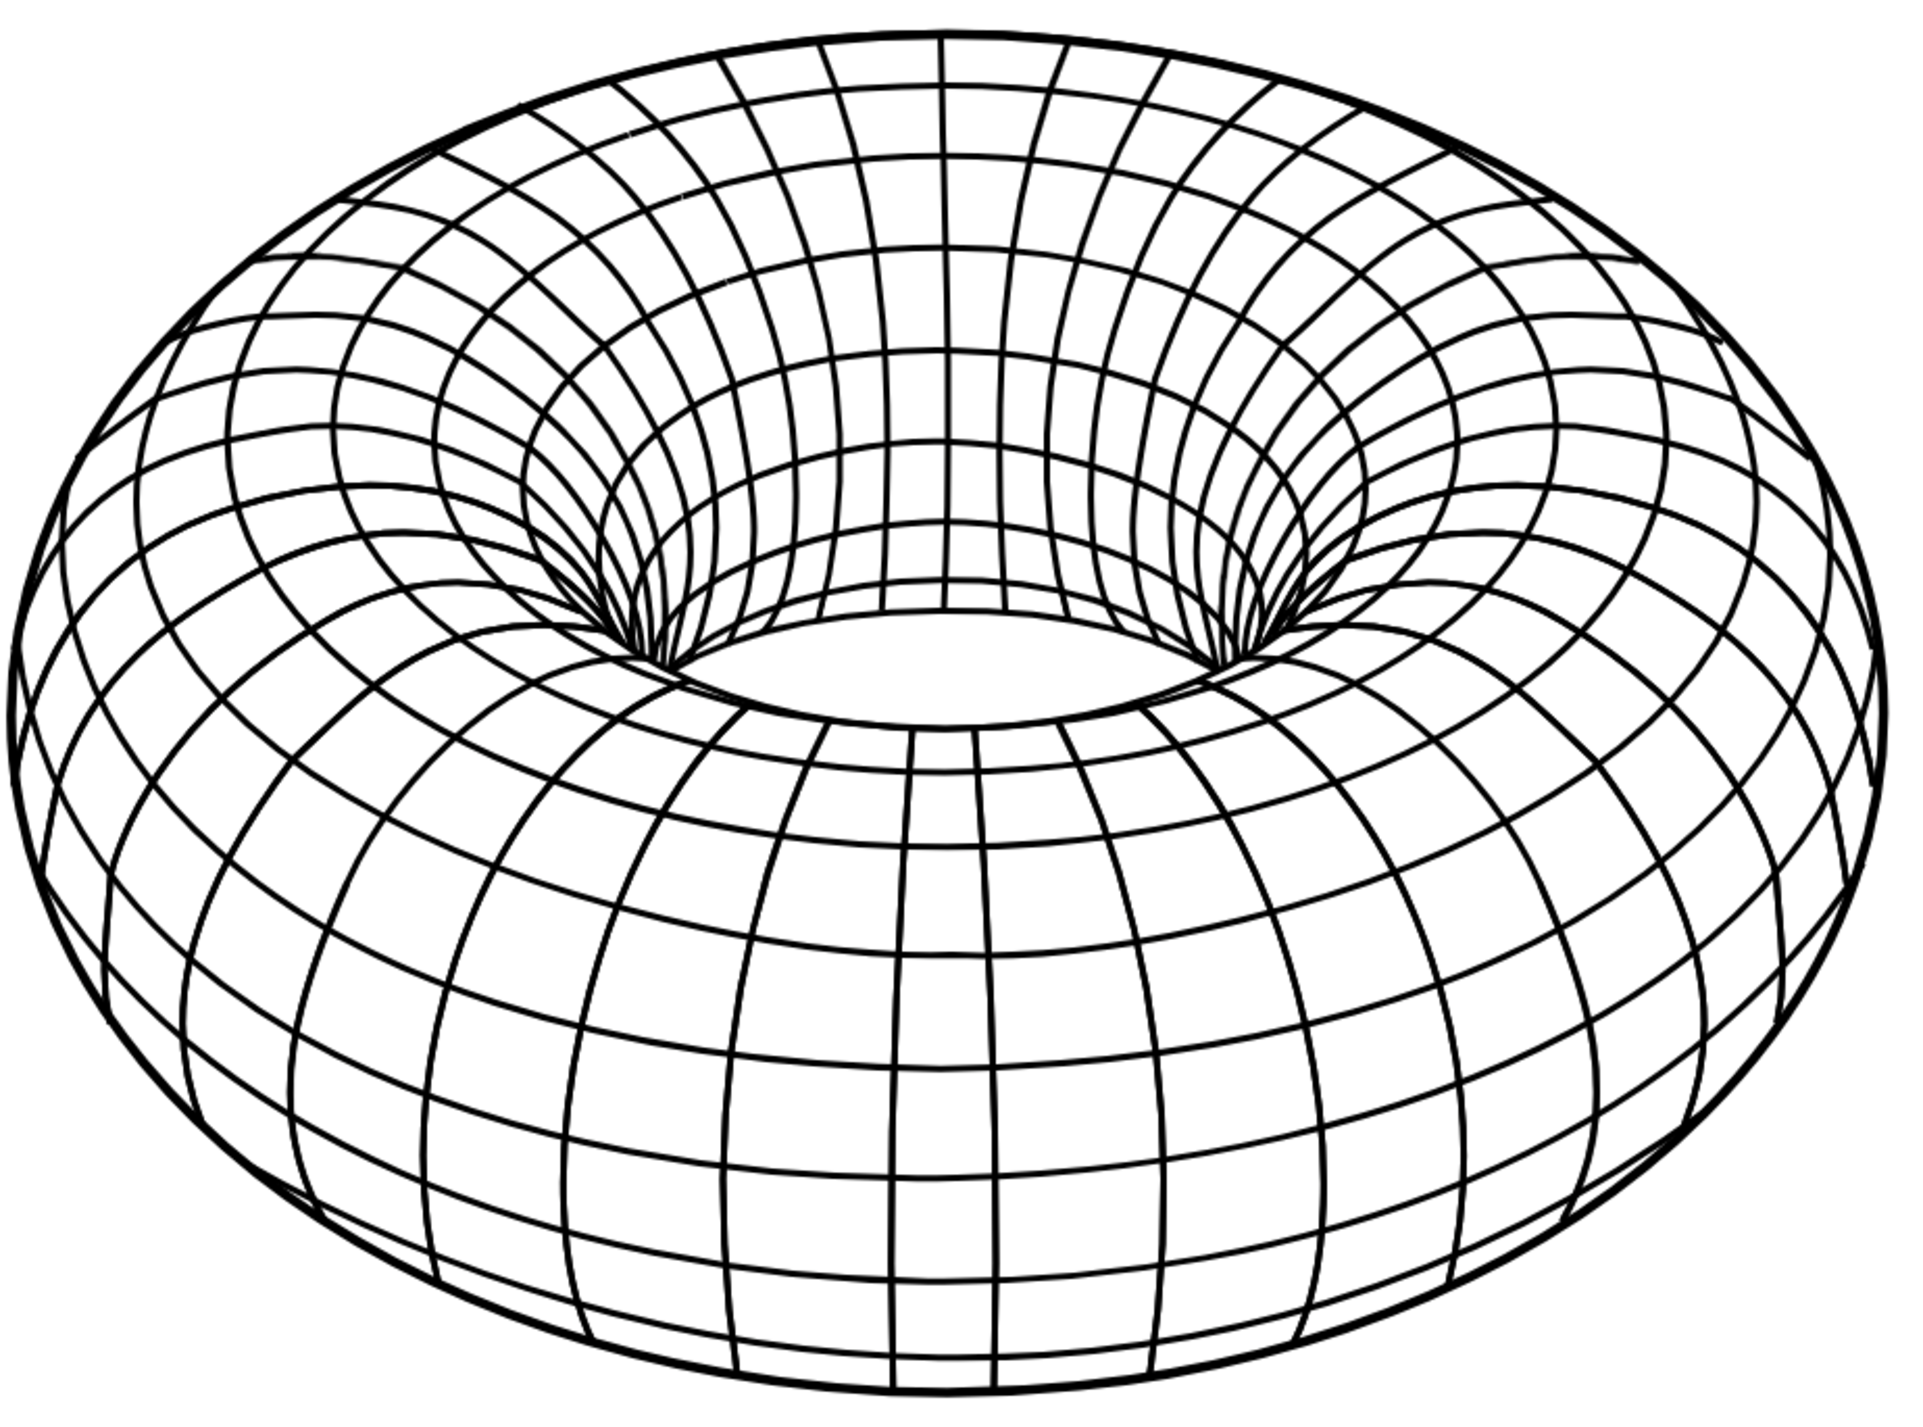
\includegraphics[width=0.45\textwidth]{torus.pdf}};
	\draw[->, very thick] (2.5,0) -- node[pos=1.4] {$y$} (3.2, 0);	
	\draw[->, very thick] (0,0) -- node[pos=1.1] {$z$} (0, 2.5);
	\draw[->, very thick] (-0.9, -0.9*4/3) -- node[pos=1.2] {$x$} (-1.5, -2);
	\end{tikzpicture}
\end{center}


To show $M$ is a hypersurface, we first compute $\nabla f$ at a general point $\ve{r} = (x,y,z) \in \mathbb{R}^3$:
\[
 \nabla_\ve{r} f = \left( \frac{2x(2 - \sqrt{x^2 + y^2)}}{\sqrt{x^2 + y^2}}, \, \frac{2y(2 - \sqrt{x^2 + y^2)}}{\sqrt{x^2 + y^2}}, \, 2z \right)
\]
Note that $\nabla f$ doesn't exist {\em everywhere} in $\mathbb{R}^3$, since there is a problem when $x^2 + y^2 = 0$ (i.e. on the $z$-axis). But for a point $\ve{p} = (a, b, c)$ on $M$, we cannot have $a^2 + b^2 = 0$ since that implies, using the equation for $M$, that
\[
 (2 - \sqrt{0})^2 + c^2 - 1 = 0,
\]
in other words, $c^2 = -3$ which is impossible. So $\nabla_\ve{p} f$ exists everywhere on $M$. Moreover, suppose $\nabla_\ve{p} f = (0,0,0)$ and $\ve{p}$ lies on $M$. Then in particular $2c = 0$ so $c=0$, and hence, using the equation for $M$, 
\[
 (2 - \sqrt{a^2 + b^2})^2 = 1
\]
which implies that $a$ and $b$ cannot both be zero. This is a contradiction, hence $\nabla_\ve{p} \neq \ve{0}$ everywhere on $M$. So $M$ is a hypersurface.
\end{solution}
\end{example}

\begin{definition} Let $M \subset \mathbb{R}^{n+1}$ be a hypersurface associated to a function $f : \mathbb{R}^{n+1} \rightarrow \mathbb{R}$. The {\em tangent space} of $M$ at $\ve{p} \in M$ is:
\[
 T_\ve{p} M := \{ \ve{v} \in \mathbb{R}^{n+1} \, : \, \nabla_\ve{p} f \dotp \ve{v} = 0 \} 
\]
\end{definition}
\begin{ramanujansays} From Multivariable Calculus, you know that we can equivalently express the tangent space to $M$ at $p$ as
\begin{align*}
T_\ve{p} M &=  \{ \ve{v} \in \mathbb{R}^{n+1} \, : \, D_\ve{v} f (\ve{p}) = 0 \} \\
&=  \left\{ \ve{v} \in \mathbb{R}^{n+1} \, : \, \frac{d}{dt}\Big|_{t=0} f(\ve{p} + t \ve{v}) = 0 \right\} 
\end{align*}
\end{ramanujansays}

\begin{lemma} If $M$ 

\end{lemma}

\begin{example} Compute a basis for the tangent space to the hyperbola $M$ from Example \ref{hyperbola_example} at $\ve{p} = (1, \sqrt{2})$. Draw a picture to illustrate the result.
\begin{solution}
We have already computed the gradient of $f$ at a point $\ve{p} = (a,b) \in M$:
\[
 \nabla_\ve{p} = (2b, -2a) \quad \mbox{ where $b^2 = 1 + a^2$}.
\]
Hence at $\ve{p} = (1, \sqrt{2})$, we have 
\[
 \nabla_\ve{p} f = (2 \sqrt{2}, -2).
\] 
Thus 
\begin{align*}
 T_\ve{p} M &= \{ (v_1, v_2) \in \mathbb{R}^2 : \nabla_\ve{p} f \dotp (v_1, v_2) = 0 \}  \\
  &= \{ (v_1, v_2) \in \mathbb{R}^2 : 2 \sqrt{2} v_1 - 2v_2 = 0  \}
\end{align*}
A basis for $T_\ve{p} M$ is $\ve{u} = (1, \frac{1}{\sqrt{2}})$. The picture is: tikzalign
\begin{center}
\begin{tikzpicture}[domain=-1.4:1.4]
\draw[<->] (-2,0) -- (2,0) node[below] {$x$};
\draw[<->] (0, -2) -- (0,2) node[right] {$y$};
\draw[very thick] plot[id=p]  ({sinh(\x)}, {cosh(\x)});
\draw[very thick] plot[id=p]  ({sinh(\x)}, {-cosh(\x)});
\draw[very thick, red] plot[id=p] ({1.5*\x}, {1/sqrt(2)*(1.5*\x) + (sqrt(2)-1/sqrt(2))}); 
\draw[very thick, fill] (1, 1.414) circle (1pt) node[below right] {$\ve{p}$};
\node at (-1.5, 1.4) {$M$};
\draw[line width=0.5mm, blue, ->] (1, 1.414) -- (1.5, 1.414 + 0.5*0.707) node[below right] {$\ve{u}$};
\end{tikzpicture}
\qquad
\begin{tikzpicture}[domain=-1.4:1.4]
\draw[<->] (-2,0) -- (2,0) node[below] {$v_1$};
\draw[<->] (0, -2) -- (0,2) node[right] {$v_2$};
\draw[very thick, red] plot[id=p] ({1.5*\x}, {1/sqrt(2)*(1.5*\x)});   
\node[red] at (2, 1.8) {$T_\ve{p} M$};
\draw[line width=0.5mm, blue, ->] (0,0) -- (0.5, 0.5*0.707) node[right, yshift=-2pt] {$\ve{u}$};
\end{tikzpicture}
\end{center}

\begin{ramanujansays} The red line in the first picture, drawn for the sake of illustration, is the tangent space shifted so that it passes through $\ve{p}$. The actual tangent space $T_\ve{p} M$ goes through the origin as in the second picture.
\end{ramanujansays}

\end{solution}
\end{example}

\end{appendices}



\backmatter
% bibliography, glossary and index would go here.


\end{document}
